\chapter{Optimering af gaslager}
Vi har indtil nu set på grafteori og algoritmer som  uafhængige teoretiske koncepter, samt hvordan algoritmer kan løse problemer indenfor grafteori. I følgende afsnit vil vi implementere dette i løsningen af vores problemstilling om optimering af et gaslager. I afsnittet om grafteori kom vi ind på forskellige aspekter herunder graftyper, grafterminologi, repræsentation af grafer, vægtede grafer og veje. Dette kan vi nu bruge til at finde den optimale vej igennem en graf for vores gaslager. I algoritmeafsnittet har vi kigget på forskellige algoritmetyper for at finde ud af, hvilken algoritme der er bedst egnet til vores problem. Vi har også kigget på kompleksitet og derudover redegjort for Dijkstras algoritme. Denne er vigtig for løsningen af vores optimeringsproblem, da man med Dijkstras algoritme kan finde den korteste vej igennem en graf. For at benytte denne på vores problem, finder vi den korteste vej igennem problemets omvendte graf, da denne vej må være den længste vej i grafen for det reelle problem, så vi maksimerer vores resultat. Længste vej-problemer er oftest NP-complete, men i vores graf, som er en orienteret, acyklisk graf, er det et P problem. Grunden til, at vi vælger at bruge Dijkstras algoritme og løser den som korteste vej, er, at den er mere optimeret end andre algoritmer, der ville kunne løse problemet som et længste vej-problem.

\section{Basisproblemet}
Vi vil indgå en lejekontrakt med ejeren af et gaslager, hvori der kan lagres naturgas. Vi vil leje dette gaslager i et år, og vi vil nu forsøge at maksimere profitten ved at købe og sælge gasenheder. Vi har en forward-kurve på prisen. En forward-kurve er en række priser, der på forhånd er aftalt med leverandørerne og køberne således, at vi til hver en tid i lejekontrakten kan se, hvad prisen for gas er til denne tid. Prisen varierer fra måned til måned. Der er desuden øvre og nedre grænser for beholdningen i gaslageret samt øvre grænser for køb og salg af gas. Ved lejekontraktens udløb vil ejeren købe den resterende gas til prisen på dette tidspunkt. Vi opstiller \autoref{table:1} med de forskellige, givne værdier, som vi skal bruge til at løse optimeringsproblemet:

\begin{table}[H]
\centering
\begin{tabular}{|c | c|} 
 \hline
 Variabel & Beskrivelse \\ [0.5ex] 
 \hline\hline
 $t$ & Tidsskridt  \\ 
 $T$ & Sluttid  \\
 $q_{t}$ & Gasenheder til tiden $t$  \\
 $\Delta q_{t}$ & Ændring i gasenheder,    $q_{t}-q_{t-1}$ \\
 $q_{0}$ & Gasenheder i starten af lejeperioden  \\
 $q_{\min}$ & Den nedre grænse for gasenheder \\ 
 $q_{\max}$ & Den øvre grænse for gasenheder \\
 $u_{\max}$ & Antal gasenheder der maksimalt kan tages ud af lageret mellem to tidsskridt \\ 
 $i_{\max}$ & Antal gasenheder der maksimalt kan sættes ind på lageret mellem to tidsskridt \\ 
 $p_{t}$ & Prisen per gasenhed ved tiden, $t$, fra forward-kurven, i euro  \\
 $r$ & En fast diskonteringsfaktor  \\
 [1ex]
 \hline
\end{tabular}
\caption{Tabel over værdier i optimeringsproblemet.}
\label{table:1}
\end{table}

I basisproblemet er $q_{\min}$, $q_{\max}$, $i_{\max}$ og $u_{\max}$ statiske. Det vil sige, at de ikke ændrer sig i hele lejeperioden. De andre værdier er variable og er dermed ikke statiske igennem lejeperioden. Det, vi i problemet ønsker at optimere, er resultatet. Problemet kan udtrykkes ved følgende funktion:
\begin{equation}
\max_{\Delta p_{t}} \Bigg\{ -\sum_{t=1}^{T} \mathrm{e}^{-r\frac{t}{T}} \Delta q_{t} p_{t}+ \mathrm{e}^{-r}q_{T}p_{T} \Bigg\}.
\end{equation}
Denne funktion har bibetingelserne:\\
1. $q_{\min} \leq q_{t} \leq q_{\max}$\\
2. $\Delta q_{t} \in \{-u_{\max},-u_{\max}+1,\dotsc,-1,0,1,\dotsc,i_{\max}-1,i_{\max} \}$ \\
for $t \in \{1,\dotsc,T\}$, hvor gasmængden lagret til tiden, $t$, er $q_{t}=q_{0}+\sum_{s=1}^{t} \Delta q_{s}$.
Det vil altså sige, at antallet af gasenheder skal ligge mellem den nedre og den øvre grænse. Ændringen i gasenheder skal ligge mellem minus det antal gasenheder, der må tages ud af gaslaget, altså det vi højst må sælge, og det antal gasenheder, der højst må sættes ind på gaslageret, altså det antal vi højst må købe.
Knuderne i grafen er skrevet på formen, $v_{t,q_t}$.

\begin{defn} [Problemgraf] \label{defn:graf_problem}
Givet problemparametrene i \autoref{table:1} defineres kanterne i grafen for problemet. Grafen, $G_{\textrm{problem}}=(V,E,w)$, er en orienteret, vægtet og simpel graf. Grafen er $(T+2)$-delt, fordelt på delmængderne $V_0,V_1, \dotsc, V_{T+1}$, hvor $V_0$ og $V_{T+1}$ kun indeholder hhv. startknuden, $v_{0,q_0}$, og slutknuden, $q_{\slut}$. Startknuden har $t=0$, da det er inden lejekontraktens begyndelse. Hver knude i en delmængde $V_t$ kan kun være nabo til en knude i delmængde $V_{t+1}$, hvor $t \in \{0,1, \dotsc,T\}$.
For $E$ gælder det, når $t<T$, at $\exists \ e = (u,v)$, hvor $u=v_{t,q_t}$ og $v=v_{t+1, q_{t+1}}$, hvis
	\begin{itemize}
	\item $u \in V_t$ og $v \in V_{t+1}$
	\item $-u_{\max} \leq \Delta q_{t+1} \leq i_{\max}$
	\item $q_{\min} \leq q_t, q_{t+1} \leq q_{\max}$,
	\end{itemize}
og hvis $t=T$, gælder det, at $\exists \ e=(u,q_{\slut})$, hvor $u=v_{T,q_T}$, hvis
	\begin{itemize}
	\item $u \in V_T$
	\item $q_{\min} \leq q_{T} \leq q_{\max}$.
	\end{itemize}
Vægten på kanterne er givet ved funktionen:
\begin{equation}
w(e)=
	\begin{cases}
	\Delta q_{t+1} \cdot p_{t+1} \cdot \textrm{e}^{-r \cdot \frac{t+1}{T}} &\text{hvis } t < T, \\
	q_T \cdot p_T \cdot \textrm{e}^{-r} & \text{ellers.}
	\end{cases}
\end{equation}

\end{defn}


\section{Grafen for basisproblemet}
Vi kan med udgangspunkt i afsnittet om grafteori opstille en graf for vores basisproblem. Grafen er en simpel, orienteret, vægtet graf. Vi opstiller et simplificeret eksempel på grafen med følgende data:
\begin{itemize}
  \item $t \in \{1,2,3,4,5,6\}$
  \item $q_{0}=1$
  \item $q_{min}=0$
  \item $q_{max}=2$
  \item $i_{max}=1$
  \item $u_{max}=1$
  \item $p_{6}=(20,22,25,18,15,15)$
\end{itemize}

I vores eksempel tager vi kun udgangspunkt i 6 måneder, og at man kun kan købe og sælge 1 gasenhed pr måned. Derudover er lageret begrænset til mindst at have nul gasenheder og højst to gasenheder. Efter de seks måneder sælger vi det gas der muligvis er på lageret til ejeren af gaslageret. Vi opstiller følgende graf med de givne vægte:

\begin{figure}[H]
\centering
	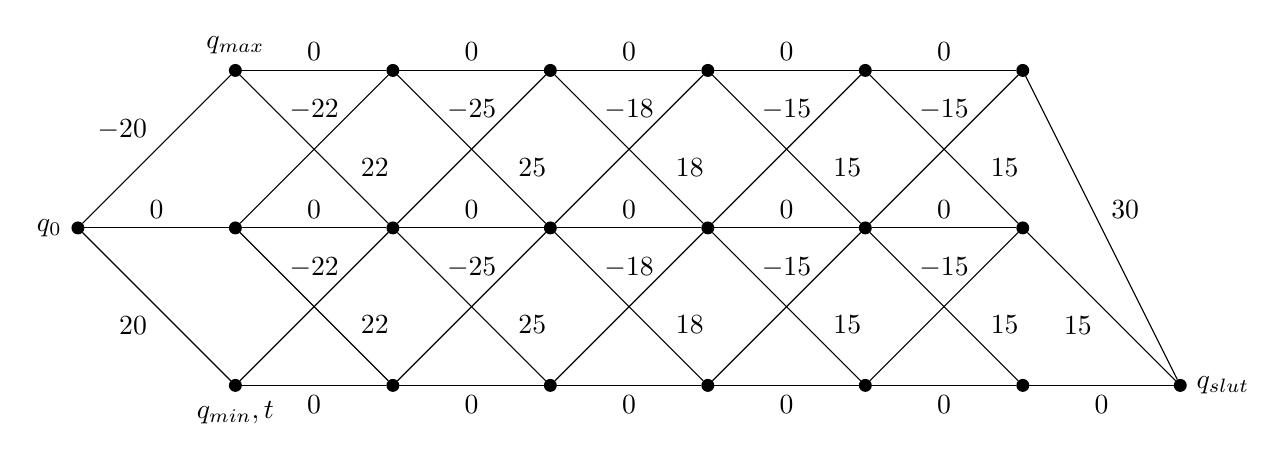
\begin{tikzpicture}

      \tikzset{enclosed/.style={draw, circle, inner sep=0pt, minimum size=.15cm, fill=black}}
%% Vertices
      	\node[enclosed, label={left: $q_{0}$}] (v1) at (0,2) {};
      	\node[enclosed, label={below: $q_{min},   t$}] (v2) at (2,0) {};
    		\node[enclosed, label={below: }] (v3) at (2,2) {};
  	    \node[enclosed, label={above: $q_{max}$}] (v4) at (2,4) {};
     	\node[enclosed, label={left: }] (v5) at (4,0) {};
     	\node[enclosed, label={left: }] (v6) at (4,2) {};
     	\node[enclosed, label={left: }] (v7) at (4,4) {};
     	\node[enclosed, label={right: }] (v8) at (6,0) {};
     	\node[enclosed, label={right: }] (v9) at (6,2) {};
     	\node[enclosed, label={right: }] (v10) at (6,4) {};
     	\node[enclosed, label={right: }] (v11) at (8,0) {};
     	\node[enclosed, label={below: }] (v12) at (8,2) {};
      	\node[enclosed, label={below: }] (v13) at (8,4) {};
  	    \node[enclosed, label={below: }] (v14) at (10,0) {};
  	    \node[enclosed, label={below: }] (v15) at (10,2) {};
     	\node[enclosed, label={below: }] (v16) at (10,4) {};
     	\node[enclosed, label={below: }] (v17) at (12,0) {};
     	 \node[enclosed, label={below:}] (v18) at (12,2) {};
     	\node[enclosed, label={below: }] (v19) at (12,4) {};
     	\node[enclosed, label={right: $q_{slut}$ }] (v20) at (14,0) {};
     	
%Edges
		\path (v1) edge node[midway, sloped, above, label={below: $20$ }] {} (v2);
		\path (v1) edge node[midway, sloped, below, label={above: $0$ }] {} (v3);
		\path (v1) edge node[midway, sloped, below, label={above: $-20$ }] {} (v4);
		\path (v2) edge node[midway, sloped, above, label={below: $0$ }] {} (v5);
		\path (v2) edge node[midway, above, label={above: $-22$ }] {} (v6);
		\path (v3) edge node[near end, sloped, below, label={above: $22$ }] {} (v5);
		\path (v3) edge node[midway, sloped, below, label={above: $0$ }] {} (v6);
		\path (v3) edge node[midway, above, label={above: $-22$ }] {} (v7);
		\path (v4) edge node[near end, sloped, below, label={above: $22$ }] {} (v6);
		\path (v4) edge node[midway, sloped, below, label={above: $0$ }] {} (v7);
		\path (v5) edge node[midway, sloped, above, label={below: $0$ }] {} (v8);
		\path (v5) edge node[midway, above, label={above: $-25$ }] {} (v9);
		\path (v6) edge node[near end, sloped, below, label={above: $25$ }] {} (v8);
		\path (v6) edge node[midway, sloped, below, label={above: $0$ }] {} (v9);
		\path (v6) edge node[midway, above, label={above: $-25$ }] {} (v10);
		\path (v7) edge node[near end, sloped, below, label={above: $25$ }] {} (v9);
		\path (v7) edge node[midway, sloped, below, label={above: $0$ }] {} (v10);
		\path (v8) edge node[midway, sloped, above, label={below: $0$ }] {} (v11);
		\path (v8) edge node[midway, above, label={above: $-18$ }] {} (v12);
		\path (v9) edge node[near end, sloped, below, label={above: $18$ }] {} (v11);
		\path (v9) edge node[midway, sloped, below, label={above: $0$ }] {} (v12);
		\path (v9) edge node[midway, above, label={above: $-18$ }] {} (v13);
		\path (v10) edge node[near end, sloped, below, label={above: $18$ }] {} (v12);
		\path (v10) edge node[midway, sloped, below, label={above: $0$ }] {} (v13);
		\path (v11) edge node[midway, sloped, above, label={below: $0$ }] {} (v14);
		\path (v11) edge node[midway, above, label={above: $-15$ }] {} (v15);
		\path (v12) edge node[near end, sloped, below, label={above: $15$ }] {} (v14);
		\path (v12) edge node[midway, sloped, below, label={above: $0$ }] {} (v15);
		\path (v12) edge node[midway, above, label={above: $-15$ }] {} (v16);
		\path (v13) edge node[near end, sloped, below, label={above: $15$ }] {} (v15);
		\path (v13) edge node[midway, sloped, below, label={above: $0$ }] {} (v16);
		\path (v14) edge node[midway, sloped, above, label={below: $0$ }] {} (v17);
		\path (v14) edge node[midway, above, label={above: $-15$ }] {} (v18);
		\path (v15) edge node[near end, sloped, below, label={above: $15$ }] {} (v17);
		\path (v15) edge node[midway, sloped, below, label={above: $0$ }] {} (v18);
		\path (v15) edge node[midway, above, label={above: $-15$ }] {} (v19);
		\path (v16) edge node[near end, sloped, below, label={above: $15$ }] {} (v18);
		\path (v16) edge node[midway, sloped, below, label={above: $0$ }] {} (v19);
		\path (v17) edge node[midway, sloped, above, label={below: $0$ }] {} (v20);
		\path (v18) edge node[midway, sloped, above, label={below: $15$ }] {} (v20);
		\path (v19) edge node[midway, sloped, below, label={above: $30$ }] {} (v20);
	\end{tikzpicture}
	\caption{Graf for forsimplet gaslager.}
	\label{fig.gaslager_graf}
\end{figure}

Hvis vi skal maksimere profitten for dette gaslager ønsker vi at finde den længste vej fra $q_{0}$ til $q_{slut}$, da vi skal have så mange penge som muligt efter lejeperioden. For at løse problemet som et korteste vej-problem og ikke et længste vej-problem ganger vi med -1. Vi opstiller dermed den omvendte graf for problemet:

\begin{figure}[H]
\centering
	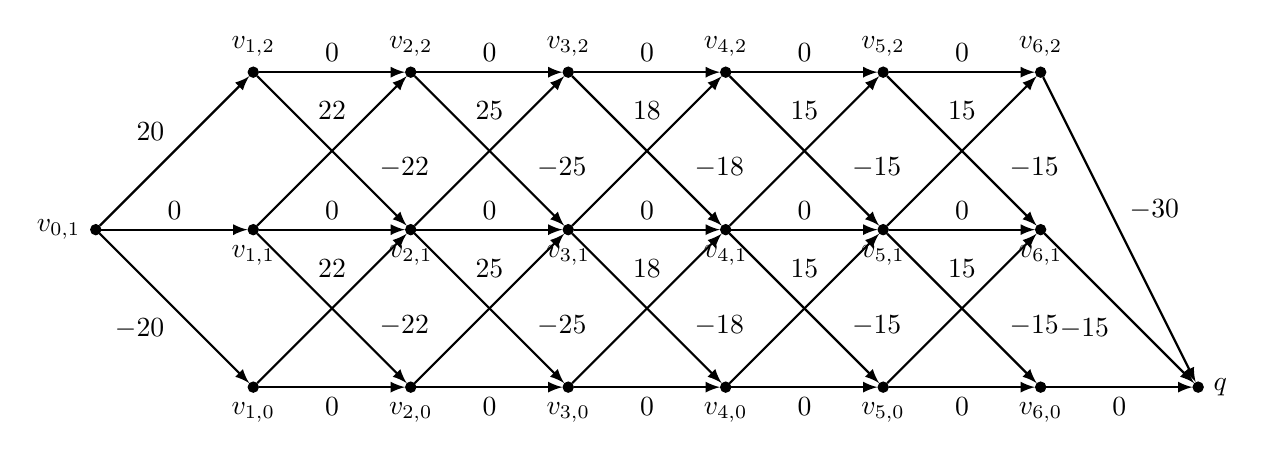
\begin{tikzpicture}

       \tikzset{enclosed/.style={draw, circle, inner sep=0pt, minimum size=.13cm, fill=black}}
%% Vertices
      	\node[enclosed, label={left: $v_{0,1}$}] (v1) at (0,2) {};
      	\node[enclosed, label={below: $v_{1,0}$}] (v2) at (2,0) {};
    		\node[enclosed, label={below: $v_{1,1}$}] (v3) at (2,2) {};
  	    \node[enclosed, label={above: $v_{1,2}$}] (v4) at (2,4) {};
     	\node[enclosed, label={below: $v_{2,0}$}] (v5) at (4,0) {};
     	\node[enclosed, label={below: $v_{2,1}$ }] (v6) at (4,2) {};
     	\node[enclosed, label={above: $v_{2,2}$}] (v7) at (4,4) {};
     	\node[enclosed, label={below:$v_{3,0}$ }] (v8) at (6,0) {};
     	\node[enclosed, label={below:$v_{3,1}$ }] (v9) at (6,2) {};
     	\node[enclosed, label={above:$v_{3,2}$ }] (v10) at (6,4) {};
     	\node[enclosed, label={below: $v_{4,0}$ }] (v11) at (8,0) {};
     	\node[enclosed, label={below:$v_{4,1}$ }] (v12) at (8,2) {};
      	\node[enclosed, label={above:$v_{4,2}$ }] (v13) at (8,4) {};
  	    \node[enclosed, label={below: $v_{5,0}$}] (v14) at (10,0) {};
  	    \node[enclosed, label={below:$v_{5,1}$ }] (v15) at (10,2) {};
     	\node[enclosed, label={above: $v_{5,2}$ }] (v16) at (10,4) {};
     	\node[enclosed, label={below:$v_{6,0}$ }] (v17) at (12,0) {};
     	 \node[enclosed, label={below:$v_{6,1}$}] (v18) at (12,2) {};
     	\node[enclosed, label={above: $v_{6,2}$}] (v19) at (12,4) {};
     	\node[enclosed, label={right: $q_{\slut}$ }] (v20) at (14,0) {};
     	
%Edges
		\path[->,>=latex,thick] (v1) edge node[midway, sloped, above, label={below: $-20$ }] {} (v2);
		\path[->,>=latex,thick] (v1) edge node[midway, sloped, below, label={above: $0$ }] {} (v3);
		\path[->,>=latex,thick] (v1) edge node[midway, sloped, below, label={above: $20$ }] {} (v4);
		\path[->,>=latex,thick] (v2) edge node[midway, sloped, above, label={below: $0$ }] {} (v5);
		\path[->,>=latex,thick] (v2) edge node[midway, above, label={above: $22$ }] {} (v6);
		\path[->,>=latex,thick] (v3) edge node[near end, sloped, below, label={above: $-22$ }] {} (v5);
		\path[->,>=latex,thick] (v3) edge node[midway, sloped, below, label={above: $0$ }] {} (v6);
		\path[->,>=latex,thick] (v3) edge node[midway, above, label={above: $22$ }] {} (v7);
		\path[->,>=latex,thick] (v4) edge node[near end, sloped, below, label={above: $-22$ }] {} (v6);
		\path[->,>=latex,thick] (v4) edge node[midway, sloped, below, label={above: $0$ }] {} (v7);
		\path[->,>=latex,thick] (v5) edge node[midway, sloped, above, label={below: $0$ }] {} (v8);
		\path[->,>=latex,thick] (v5) edge node[midway, above, label={above: $25$ }] {} (v9);
		\path[->,>=latex,thick] (v6) edge node[near end, sloped, below, label={above: $-25$ }] {} (v8);
		\path[->,>=latex,thick] (v6) edge node[midway, sloped, below, label={above: $0$ }] {} (v9);
		\path[->,>=latex,thick] (v6) edge node[midway, above, label={above: $25$ }] {} (v10);
		\path[->,>=latex,thick] (v7) edge node[near end, sloped, below, label={above: $-25$ }] {} (v9);
		\path[->,>=latex,thick] (v7) edge node[midway, sloped, below, label={above: $0$ }] {} (v10);
		\path[->,>=latex,thick] (v8) edge node[midway, sloped, above, label={below: $0$ }] {} (v11);
		\path[->,>=latex,thick] (v8) edge node[midway, above, label={above: $18$ }] {} (v12);
		\path[->,>=latex,thick] (v9) edge node[near end, sloped, below, label={above: $-18$ }] {} (v11);
		\path[->,>=latex,thick] (v9) edge node[midway, sloped, below, label={above: $0$ }] {} (v12);
		\path[->,>=latex,thick] (v9) edge node[midway, above, label={above: $18$ }] {} (v13);
		\path[->,>=latex,thick] (v10) edge node[near end, sloped, below, label={above: $-18$ }] {} (v12);
		\path[->,>=latex,thick] (v10) edge node[midway, sloped, below, label={above: $0$ }] {} (v13);
		\path[->,>=latex,thick] (v11) edge node[midway, sloped, above, label={below: $0$ }] {} (v14);
		\path[->,>=latex,thick] (v11) edge node[midway, above, label={above: $15$ }] {} (v15);
		\path[->,>=latex,thick] (v12) edge node[near end, sloped, below, label={above: $-15$ }] {} (v14);
		\path[->,>=latex,thick] (v12) edge node[midway, sloped, below, label={above: $0$ }] {} (v15);
		\path[->,>=latex,thick] (v12) edge node[midway, above, label={above: $15$ }] {} (v16);
		\path[->,>=latex,thick] (v13) edge node[near end, sloped, below, label={above: $-15$ }] {} (v15);
		\path[->,>=latex,thick] (v13) edge node[midway, sloped, below, label={above: $0$ }] {} (v16);
		\path[->,>=latex,thick] (v14) edge node[midway, sloped, above, label={below: $0$ }] {} (v17);
		\path[->,>=latex,thick] (v14) edge node[midway, above, label={above: $15$ }] {} (v18);
		\path[->,>=latex,thick] (v15) edge node[near end, sloped, below, label={above: $-15$ }] {} (v17);
		\path[->,>=latex,thick] (v15) edge node[midway, sloped, below, label={above: $0$ }] {} (v18);
		\path[->,>=latex,thick] (v15) edge node[midway, above, label={above: $15$ }] {} (v19);
		\path[->,>=latex,thick] (v16) edge node[near end, sloped, below, label={above: $-15$ }] {} (v18);
		\path[->,>=latex,thick] (v16) edge node[midway, sloped, below, label={above: $0$ }] {} (v19);
		\path[->,>=latex,thick] (v17) edge node[midway, sloped, above, label={below: $0$ }] {} (v20);
		\path[->,>=latex,thick] (v18) edge node[midway, sloped, above, label={below: $-15$ }] {} (v20);
		\path[->,>=latex,thick] (v19) edge node[midway, sloped, below, label={above: $-30$ }] {} (v20);
	\end{tikzpicture}
	\caption{Graf for forsimplet gaslager ganget med -1.}
	\label{fig.gaslager_graf}
\end{figure}

Vi kan nu løse problemet som et korteste vej-problem. Dertil vil vi bruge Dijkstras algoritme. Dette kan dog ikke lade sig gøre så længe, at der optræder ikke-positive tal i grafen. Derfor lægger vi 30 til alle tal i grafen, således at det mindste tal bliver nul. Vi får nu den omvendte graf med positive kantvægte:


\begin{figure}[H]
\centering
	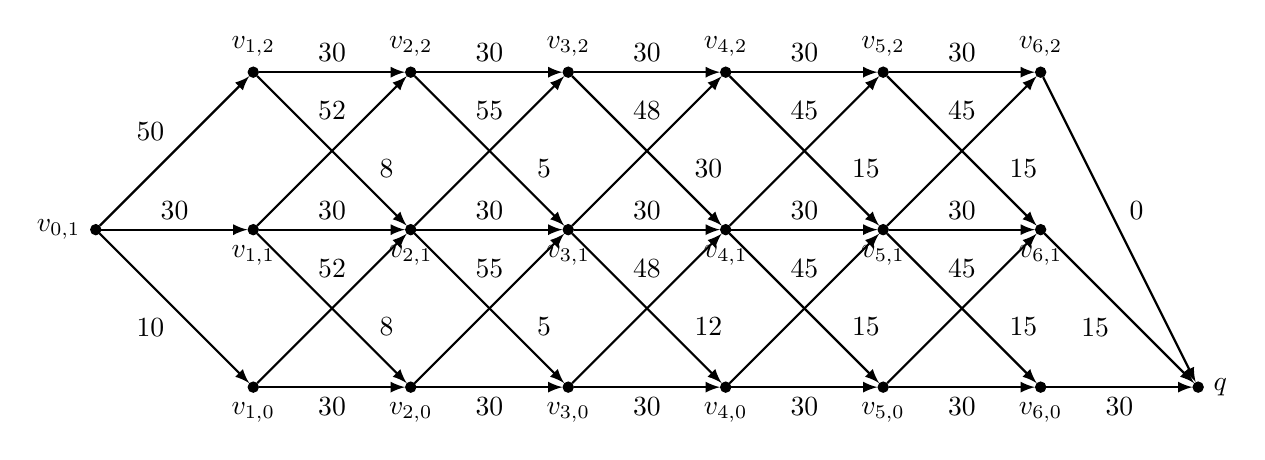
\begin{tikzpicture}

       \tikzset{enclosed/.style={draw, circle, inner sep=0pt, minimum size=.13cm, fill=black}}
%% Vertices
      	\node[enclosed, label={left: $v_{0,1}$}] (v1) at (0,2) {};
      	\node[enclosed, label={below: $v_{1,0}$}] (v2) at (2,0) {};
    		\node[enclosed, label={below: $v_{1,1}$}] (v3) at (2,2) {};
  	    \node[enclosed, label={above: $v_{1,2}$}] (v4) at (2,4) {};
     	\node[enclosed, label={below: $v_{2,0}$}] (v5) at (4,0) {};
     	\node[enclosed, label={below: $v_{2,1}$ }] (v6) at (4,2) {};
     	\node[enclosed, label={above: $v_{2,2}$}] (v7) at (4,4) {};
     	\node[enclosed, label={below:$v_{3,0}$ }] (v8) at (6,0) {};
     	\node[enclosed, label={below:$v_{3,1}$ }] (v9) at (6,2) {};
     	\node[enclosed, label={above:$v_{3,2}$ }] (v10) at (6,4) {};
     	\node[enclosed, label={below: $v_{4,0}$ }] (v11) at (8,0) {};
     	\node[enclosed, label={below:$v_{4,1}$ }] (v12) at (8,2) {};
      	\node[enclosed, label={above:$v_{4,2}$ }] (v13) at (8,4) {};
  	    \node[enclosed, label={below: $v_{5,0}$}] (v14) at (10,0) {};
  	    \node[enclosed, label={below:$v_{5,1}$ }] (v15) at (10,2) {};
     	\node[enclosed, label={above: $v_{5,2}$ }] (v16) at (10,4) {};
     	\node[enclosed, label={below:$v_{6,0}$ }] (v17) at (12,0) {};
     	 \node[enclosed, label={below:$v_{6,1}$}] (v18) at (12,2) {};
     	\node[enclosed, label={above: $v_{6,2}$}] (v19) at (12,4) {};
     	\node[enclosed, label={right: $q_{\slut}$ }] (v20) at (14,0) {};
     	
%Edges
		\path[->,>=latex,thick] (v1) edge node[midway, sloped, above, label={below: $10$ }] {} (v2);
		\path[->,>=latex,thick] (v1) edge node[midway, sloped, below, label={above: $30$ }] {} (v3);
		\path[->,>=latex,thick] (v1) edge node[midway, sloped, below, label={above: $50$ }] {} (v4);
		\path[->,>=latex,thick] (v2) edge node[midway, sloped, above, label={below: $30$ }] {} (v5);
		\path[->,>=latex,thick] (v2) edge node[midway, above, label={above: $52$ }] {} (v6);
		\path[->,>=latex,thick] (v3) edge node[near end, sloped, below, label={above: $8$ }] {} (v5);
		\path[->,>=latex,thick] (v3) edge node[midway, sloped, below, label={above: $30$ }] {} (v6);
		\path[->,>=latex,thick] (v3) edge node[midway, above, label={above: $52$ }] {} (v7);
		\path[->,>=latex,thick] (v4) edge node[near end, sloped, below, label={above: $8$ }] {} (v6);
		\path[->,>=latex,thick] (v4) edge node[midway, sloped, below, label={above: $30$ }] {} (v7);
		\path[->,>=latex,thick] (v5) edge node[midway, sloped, above, label={below: $30$ }] {} (v8);
		\path[->,>=latex,thick] (v5) edge node[midway, above, label={above: $55$ }] {} (v9);
		\path[->,>=latex,thick] (v6) edge node[near end, sloped, below, label={above: $5$ }] {} (v8);
		\path[->,>=latex,thick] (v6) edge node[midway, sloped, below, label={above: $30$ }] {} (v9);
		\path[->,>=latex,thick] (v6) edge node[midway, above, label={above: $55$ }] {} (v10);
		\path[->,>=latex,thick] (v7) edge node[near end, sloped, below, label={above: $5$ }] {} (v9);
		\path[->,>=latex,thick] (v7) edge node[midway, sloped, below, label={above: $30$ }] {} (v10);
		\path[->,>=latex,thick] (v8) edge node[midway, sloped, above, label={below: $30$ }] {} (v11);
		\path[->,>=latex,thick] (v8) edge node[midway, above, label={above: $48$ }] {} (v12);
		\path[->,>=latex,thick] (v9) edge node[near end, sloped, below, label={above: $12$ }] {} (v11);
		\path[->,>=latex,thick] (v9) edge node[midway, sloped, below, label={above: $30$ }] {} (v12);
		\path[->,>=latex,thick] (v9) edge node[midway, above, label={above: $48$ }] {} (v13);
		\path[->,>=latex,thick] (v10) edge node[near end, sloped, below, label={above: $30$ }] {} (v12);
		\path[->,>=latex,thick] (v10) edge node[midway, sloped, below, label={above: $30$ }] {} (v13);
		\path[->,>=latex,thick] (v11) edge node[midway, sloped, above, label={below: $30$ }] {} (v14);
		\path[->,>=latex,thick] (v11) edge node[midway, above, label={above: $45$ }] {} (v15);
		\path[->,>=latex,thick] (v12) edge node[near end, sloped, below, label={above: $15$ }] {} (v14);
		\path[->,>=latex,thick] (v12) edge node[midway, sloped, below, label={above: $30$ }] {} (v15);
		\path[->,>=latex,thick] (v12) edge node[midway, above, label={above: $45$ }] {} (v16);
		\path[->,>=latex,thick] (v13) edge node[near end, sloped, below, label={above: $15$ }] {} (v15);
		\path[->,>=latex,thick] (v13) edge node[midway, sloped, below, label={above: $30$ }] {} (v16);
		\path[->,>=latex,thick] (v14) edge node[midway, sloped, above, label={below: $30$ }] {} (v17);
		\path[->,>=latex,thick] (v14) edge node[midway, above, label={above: $45$ }] {} (v18);
		\path[->,>=latex,thick] (v15) edge node[near end, sloped, below, label={above: $15$ }] {} (v17);
		\path[->,>=latex,thick] (v15) edge node[midway, sloped, below, label={above: $30$ }] {} (v18);
		\path[->,>=latex,thick] (v15) edge node[midway, above, label={above: $45$ }] {} (v19);
		\path[->,>=latex,thick] (v16) edge node[near end, sloped, below, label={above: $15$ }] {} (v18);
		\path[->,>=latex,thick] (v16) edge node[midway, sloped, below, label={above: $30$ }] {} (v19);
		\path[->,>=latex,thick] (v17) edge node[midway, sloped, above, label={below: $30$ }] {} (v20);
		\path[->,>=latex,thick] (v18) edge node[midway, sloped, above, label={below: $15$ }] {} (v20);
		\path[->,>=latex,thick] (v19) edge node[midway, sloped, below, label={above: $0$ }] {} (v20);
	\end{tikzpicture}
	\caption{Graf for forsimplet gaslager ganget med -1 og med positive vægte.}
	\label{fig.gaslager_graf}
\end{figure}

Vi vil nu opstille en tabel over de mulige veje gennem grafen fra $q_0$ til $q_slut$ Denne tabel tager udgangspunkt i Eksempel \ref{exmp.dijkstae}.

\begin{table}[H]
\centering
\begin{tabular}{|c|c|c|c|c|c|c|c|c|c|c|c|c|c|} 
\hline
$k$ & $S_{k} \bigcup$ & $q_{0}$ & $v_{1,1}$ & $v_{1,2}$ & $v_{1,3}$ & $v_{2,1}$ & $v_{2,2}$ & $v_{2,3}$ & $\ldots$ & $v_{6,1}$ & $v_{6,2}$ & $v_{6,3}$ & $q_{/slut}$ \\
\hline
0 & $\emptyset$ & 0 & $\infty$ & $\infty$ & $\infty$ & $\infty$ & $\infty$ & $\infty$ & $\ldots$ & $\infty$ & $\infty$ & $\infty$ & $\infty$ \\ 
1 & $q_{0}$ & & 10 & 30 & 50 & $\infty$ & $\infty$ & $\infty$ & $\ldots$ & $\infty$ & $\infty$ & $\infty$ & $\infty$\\ 
2 & $v_{1,1}$ & & & 30 & 50 & 40 & 62 & $\infty$ & $\ldots$ & $\infty$ & $\infty$ & $\infty$ & $\infty$\\ 
3 & $v_{1,2}$ & & & & 50 & 38 & 60 & 82 & $\ldots$ & $\infty$ & $\infty$ & $\infty$ & $\infty$\\
4 & $v_{1,3}$ & & & & & 38 & 58 & 80 & $\ldots$ & $\infty$ & $\infty$ & $\infty$ & $\infty$\\ 
5 & $v_{2,1}$ & & & & & & 58 & 80 & $\ldots$ & $\infty$ & $\infty$ & $\infty$ & $\infty$\\ 
6 & $v_{2,2}$ & & & & & & & 80 & $\ldots$ & $\infty$ & $\infty$ & $\infty$ & $\infty$\\  
$\vdots$ & $\vdots$ & $\vdots$ & $\vdots$ & $\vdots$ & $\vdots$ & $\vdots$ & $\vdots$ & $\vdots$ &  & $\vdots$ & $\vdots$ & $\vdots$ & $\vdots$\\ 
14 & $v_{5,1}$ &  &  &  &  &  &  &  & $\ldots$ & 153 & 168 & $\infty$ & $\infty$\\ 
15 & $v_{5,2}$ &  &  &  &  &  &  &  & $\ldots$ & 153 & 168 & 183 & $\infty$\\ 
16 & $v_{5,3}$ &  &  &  &  &  &  &  & $\ldots$ & 153 & 168 & 183 & $\infty$\\ 
17 & $v_{6,1}$ &  &  &  &  &  &  &  & $\ldots$ &  & 168 & 183 & 183\\ 
18 & $v_{6,2}$ &  &  &  &  &  &  &  & $\ldots$ &  &  & 183 & 183\\ 
18 & $v_{6,3}$ &  &  &  &  &  &  &  & $\ldots$ &  &  &  & 183\\ 
\hline
\end{tabular}
\caption{Tabel over veje gennem forsimplet graf.}
\label{table:forsimplet_graf}
\end{table} 


Det ses, at $q_0$ har længden nul, da dette blot er startknuden. Fra $q_0$ går der tre veje til henholdsvis $v_{1,1}$, $v_{1,2}$ og $v_{1,3}$, med længderne 10, 30 og 50. Vejene til resten af knuderne i grafen er uendelig, da de endnu ikke indgår i mængden, $S$, og vi dermed ikke ved hvor langt, der er til disse knuder. Vi kigger nu på $v_{1,1}$, og ser hvilke muligheder for veje, som vi nu har. Vi har stadig $P=(q_{0},v_{1,2})=30$ og $P=(q_{0},v_{1,3})=50$, og de nye veje igennem $v_{1,1}$ giver nu mulighederne: $P=(q_{0},v_{1,1},v_{2,1})=40$ og $P=(q_{0},v_{1,1},v_{2,2})=62$. Går vi herefter videre med $v_{1,2}$, som nu er den korteste vej, får vi på samme måde vejene: $P=(q_{0},v_{1,3})=50$, $P=(q_{0},v_{1,2},v_{2,1})=38$, $P=(q_{0},v_{1,2},v_{2,2})=60$ og $P=(q_{0},v_{1,2},v_{2,3})=82$. Vi har nu to forskellige veje fra $q_{0}$ til $v_{2,1}$ og to veje fra $q_{0}$ til $v_{2,2}$. Vi ser at vejene gående igennem $v_{1,2}$ og til begge punkter er kortere end vejende gående igennem $v_{1,1}$. Derfor er det denne vej vi kører videre med, da vi ønsker at finde den korteste vej til hvert punkt for dermed at finde den korteste vej igennem grafen. På denne måde fortsætter vi igennem grafen. Det ses, at vi har tre forskellige veje til $q_slut$, som alle er 183 lang. Hvis vi tænker på den oprindelige graf, havde kanterne andre vægte, hvilket vi nu kan indsætte igen efter brugen af Dijkstras algoritme. Vejen er igennem de samme punkter, og ønsker vi at finde distancen fra $q_{0}$ til $q_{slut}$ skal vi blot tage vores resultat og trække de 30 fra igen 7 gange, altså en for hver måned samt vejen hen til $q_{slut}$. Derefter ganger vi med -1.
\begin{equation}
(183-30 \cdot 7) \cdot (-1) = 27
\end{equation}
Vejene illustreres på \autoref{fig.gaslager_graf}:

\begin{figure}[H]
\centering
	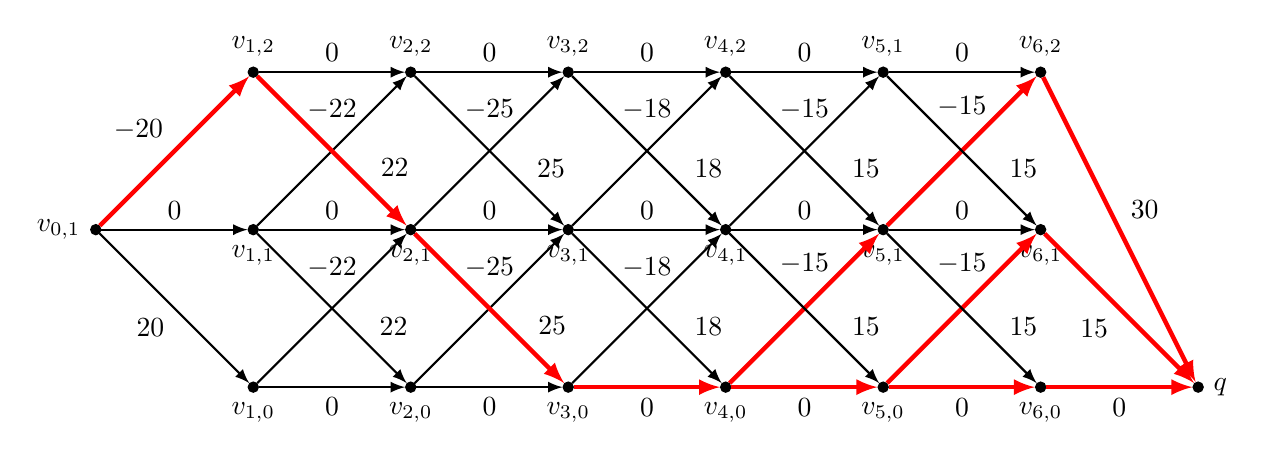
\begin{tikzpicture}

       \tikzset{enclosed/.style={draw, circle, inner sep=0pt, minimum size=.13cm, fill=black}}
%% Vertices
      	\node[enclosed, label={left: $v_{0,1}$}] (v1) at (0,2) {};
      	\node[enclosed, label={below: $v_{1,0}$}] (v2) at (2,0) {};
    		\node[enclosed, label={below: $v_{1,1}$}] (v3) at (2,2) {};
  	    \node[enclosed, label={above: $v_{1,2}$}] (v4) at (2,4) {};
     	\node[enclosed, label={below: $v_{2,0}$}] (v5) at (4,0) {};
     	\node[enclosed, label={below: $v_{2,1}$ }] (v6) at (4,2) {};
     	\node[enclosed, label={above: $v_{2,2}$}] (v7) at (4,4) {};
     	\node[enclosed, label={below:$v_{3,0}$ }] (v8) at (6,0) {};
     	\node[enclosed, label={below:$v_{3,1}$ }] (v9) at (6,2) {};
     	\node[enclosed, label={above:$v_{3,2}$ }] (v10) at (6,4) {};
     	\node[enclosed, label={below: $v_{4,0}$ }] (v11) at (8,0) {};
     	\node[enclosed, label={below:$v_{4,1}$ }] (v12) at (8,2) {};
      	\node[enclosed, label={above:$v_{4,2}$ }] (v13) at (8,4) {};
  	    \node[enclosed, label={below: $v_{5,0}$}] (v14) at (10,0) {};
  	    \node[enclosed, label={below:$v_{5,1}$ }] (v15) at (10,2) {};
     	\node[enclosed, label={above: $v_{5,1}$ }] (v16) at (10,4) {};
     	\node[enclosed, label={below:$v_{6,0}$ }] (v17) at (12,0) {};
     	 \node[enclosed, label={below:$v_{6,1}$}] (v18) at (12,2) {};
     	\node[enclosed, label={above: $v_{6,2}$}] (v19) at (12,4) {};
     	\node[enclosed, label={right: $q_{\slut}$ }] (v20) at (14,0) {};
     	
%Edges
		\path[->,>=latex,thick] (v1) edge node[midway, sloped, above, label={below, black: $20$}] {} (v2);
		\path[->,>=latex,thick] (v1) edge node[midway, sloped, below, label={above: $0$ }] {} (v3);
		\path[red,->,>=latex,ultra thick] (v1) edge node[midway, sloped, below, label={above, black: $-20$ }] {} (v4);
		\path[->,>=latex,thick] (v2) edge node[midway, sloped, above, label={below: $0$ }] {} (v5);
		\path[->,>=latex,thick] (v2) edge node[midway, above, label={above: $-22$ }] {} (v6);
		\path[->,>=latex,thick] (v3) edge node[near end, sloped, below, label={above: $22$ }] {} (v5);
		\path[->,>=latex,thick] (v3) edge node[midway, sloped, below, label={above: $0$ }] {} (v6);
		\path[->,>=latex,thick] (v3) edge node[midway, above, label={above: $-22$ }] {} (v7);
		\path[red,->,>=latex,ultra thick] (v4) edge node[near end, sloped, below, label={above, black: $22$ }] {} (v6);
		\path[->,>=latex,thick] (v4) edge node[midway, sloped, below, label={above: $0$ }] {} (v7);
		\path[->,>=latex,thick] (v5) edge node[midway, sloped, above, label={below: $0$ }] {} (v8);
		\path[->,>=latex,thick] (v5) edge node[midway, above, label={above: $-25$ }] {} (v9);
		\path[red,->,>=latex,ultra thick] (v6) edge node[near end, sloped, below, label={above,black: $25$ }] {} (v8);
		\path[->,>=latex,thick] (v6) edge node[midway, sloped, below, label={above: $0$ }] {} (v9);
		\path[->,>=latex,thick] (v6) edge node[midway, above, label={above: $-25$ }] {} (v10);
		\path[->,>=latex,thick] (v7) edge node[near end, sloped, below, label={above: $25$ }] {} (v9);
		\path[->,>=latex,thick] (v7) edge node[midway, sloped, below, label={above: $0$ }] {} (v10);
		\path[red,->,>=latex,ultra thick] (v8) edge node[midway, sloped, above, label={below,black: $0$ }] {} (v11);
		\path[->,>=latex,thick] (v8) edge node[midway, above, label={above: $-18$ }] {} (v12);
		\path[->,>=latex,thick] (v9) edge node[near end, sloped, below, label={above: $18$ }] {} (v11);
		\path[->,>=latex,thick] (v9) edge node[midway, sloped, below, label={above: $0$ }] {} (v12);
		\path[->,>=latex,thick] (v9) edge node[midway, above, label={above: $-18$ }] {} (v13);
		\path[->,>=latex,thick] (v10) edge node[near end, sloped, below, label={above: $18$ }] {} (v12);
		\path[->,>=latex,thick] (v10) edge node[midway, sloped, below, label={above: $0$ }] {} (v13);
		\path[red,->,>=latex,ultra thick] (v11) edge node[midway, sloped, above, label={below,black: $0$ }] {} (v14);
		\path[red,->,>=latex,ultra thick] (v11) edge node[midway, above, label={above,black: $-15$ }] {} (v15);
		\path[->,>=latex,thick] (v12) edge node[near end, sloped, below, label={above: $15$ }] {} (v14);
		\path[->,>=latex,thick] (v12) edge node[midway, sloped, below, label={above: $0$ }] {} (v15);
		\path[->,>=latex,thick] (v12) edge node[midway, above, label={above: $-15$ }] {} (v16);
		\path[->,>=latex,thick] (v13) edge node[near end, sloped, below, label={above: $15$ }] {} (v15);
		\path[->,>=latex,thick] (v13) edge node[midway, sloped, below, label={above: $0$ }] {} (v16);
		\path[red,->,>=latex,ultra thick] (v14) edge node[midway, sloped, above, label={below,black: $0$ }] {} (v17);
		\path[red,->,>=latex,ultra thick] (v14) edge node[midway, above, label={above,black: $-15$ }] {} (v18);
		\path[->,>=latex,thick] (v15) edge node[near end, sloped, below, label={above: $15$ }] {} (v17);
		\path[->,>=latex,thick] (v15) edge node[midway, sloped, below, label={above: $0$ }] {} (v18);
		\path[red,->,>=latex,ultra thick] (v15) edge node[midway, above, label={above,black: $-15$ }] {} (v19);
		\path[->,>=latex,thick] (v16) edge node[near end, sloped, below, label={above: $15$ }] {} (v18);
		\path[->,>=latex,thick] (v16) edge node[midway, sloped, below, label={above: $0$ }] {} (v19);
		\path[red,->,>=latex,ultra thick] (v17) edge node[midway, sloped, above, label={below,black: $0$ }] {} (v20);
		\path[red,->,>=latex,ultra thick] (v18) edge node[midway, sloped, above, label={below,black: $15$ }] {} (v20);
		\path[red,->,>=latex,ultra thick] (v19) edge node[midway, sloped, below, label={above,black: $30$ }] {} (v20);
	\end{tikzpicture}
	\caption{Længste vej igennem grafen.}
	\label{fig.gaslager_graf}
\end{figure}



\section{Basisproblemet som algoritme}
For at løse vores basisproblem, ønsker vi at opstille en algoritme, som kan finde den vej gennem grafen, der giver den største profit. Vores algoritme vil tage udgangspunkt i \autoref{alg:dijkstra}. Vi deler algoritmen op i mindre dele, for at give et bedre overblik og for bedre at kunne forklare de enkelte dele. Vi starter med at opskrive de givne data. 

\begin{algorithm}[H] 
\caption{Algoritmens data}
\begin{algorithmic}[1]
\State $q_{min}=0$
\State $q_{min\_liste}=[0,0,0,4,4,6,6,4,4,0,0,0]$
\State $q_{max}=10$
\State $q_{max\_liste}=[10,10,10,10,8,8,8,8,10,10,10,10]$
\State $i_{max}=4$
\State $i_{max\_liste}=[4,4,2,2,1,1,1,1,2,2,4,4]$
\State $u_{max}=4$
\State $u_{max\_liste}=[4,4,2,2,1,1,1,1,2,2,4,4]$
\State $gaspriser=[20,22,25,18,15,15,20,19,21,12,22,25]$
\State $q_{0}=5$
\State $r=0.04$
\State $T=12$
\State $q_{goal}=5$
\State $straffaktor=0.7$

\end{algorithmic}
\label{alg:basis}
\end{algorithm}

Værdierne er alle givet i basisproblemet.
Dernæst vil vi finde de reelle værdier for forwardpriserne i forhold til nutidsværdien. Vi laver først en liste, som vi kalder interest, som udregner hvor meget mindre værd pengene er til tiden t med vores diskonteringsfaktor, $r$. Derefter kan vi bruge denne liste til at beregne de reelle værdier for forwardpriserne.

\begin{lstlisting} [label=interest,caption=Reelle værdier for forwardpriserne]
def interest():
	interest_rate=[]
	for i in t:
		interest_i=np.e**(-r*i/T)
		interest_rate.append(interest_i)
	return interest rate
	
def get_interest_price():
	interest_price=[]
	for i in range (len(t)):
		a=interest()[i]*p_t[i]
		interest_price.append(a)
	return interest_price

\end{lstlisting}
Her dannes først en tom liste over diskonteringsværdier. Derefter sættes en forløkke i gang som beregner disse for alle værdier for $t$. Herefter laver vi en ny funktion, som danner en tom liste med de reelle værdier for forwardpriserne. Her sættes også en forløkke igang, som tilføjer værdier til denne liste ved at bruge funktionen for diskonteringsværdierne, og for hver værdi, $i$, gange diskonteringsværdien med prisen til $t$. På denne måde har vi nu dannet en liste over de reelle værdier for hvert $t$. Disse priser vil vi senere bruge i vores specificerede Dijkstra-algoritme. Først vil vi dog opstille en nabomatrix over vores basisproblemgraf, så vi kan bruge disse knuder i vores algoritme. Vi danner nabomatrixen:

\begin{lstlisting} [label=nabomatrix_kode,caption=Nabomatrix for vores problemgraf]
def graph_matrix()	
	infinity=99999
	for i in range(T)
		graph=[[infinity]*(q_max+1)]
		vertices= copy.deepcopy(graph)  #kopierer graph
		vertices.append ( [ 0 ] )
		vertices.reverse()
	return vertices
\end{lstlisting}

Nu kan vi så begynde at opstille den funktion, der ved hjælp af Dijkstras algoritme kan beregne den korteste vej:

\begin{lstlisting} [label=dijkstra_kode_problem,caption=Dijkstras algoritme for vores problem]
def dijkstras(q_t):
	oevre_graense=q_t+i_max
	if oevre_graense>q_max:
		oevre_graense=q_max
	nedre_graense=q_t-u_max
	if nedre_graense<q_min
		nedre_graense=q_min
	path=[]	
	for t in range (T)
		if t==0:
			for i in range (nedre_graense,oevre_graense+1):
				infinity=99999
				if graf[t+1][i]=infinity:
					graf[t+1][i]=interest_price[t]
					path[t][i]=q_t-i
		else:
			for i in range (nedre_graense,oevre_graense+1):
				if graf[t][q_t+interest_price[t]*(q_t-i)]>graf[t+1][i]
					graf[t+1][i]=graf[t][q_t]+interest_price[t]*(q_t-1)
					path[t][i]=q_t-i
\end{lstlisting}

Vi starter med at finde grænserne for hvor længe vores løkker senere i kildekoden skal køre. Vi bestemmer først den øvre værdi ved at tage den nuværende mængde gasenheder til tiden $t$ og lægge det sammen med den øvre grænse for det antal gasenheder, der kan sættes ind på lageret mellem to tidsskridt. Hvis den beregnede øvre grænse bliver større end den reelle øvre grænse for lagerbeholdningen i gaslageret, $q_{max}$, sætter vi dog værdien for den øvre grænse til at være $q_{max}$. På samme måde finder vi den nedre grænse ved at tage den nuværende mængde gasenheder til tiden $t$ og trække det antal gasenheder, der højst må tages ud af lageret mellem to tidsskridt fra. Hvis den beregnede nedre grænse bliver mindre end den reelle nedre grænse for lagerbeholdningen i gaslageret, $q_{min}$, sætter vi dog værdien for den nedre grænse til at være $q_{min}$. Derefter ser vi, om $t=0$. Hvis dette er tilfældet laver vi en forløkke, der kører fra den nedre til den øvre grænse$+1$, og vi definerer uendeligt til at være 99999. Hvis punktet i grafen på plads $[t+1][i]$ er minus uendelig, altså at den endnu ikke optræder i vejen, sætter vi punktet på denne plads til at være den reelle pris på gas til den tid, og til vejen tilføres på plads [t][i] den mængde gasenheder der er til tiden $t$ minus i. Hvis $t$ derimod ikke er lig nul kører en anden forløkke med de samme grænser. Her sammenlignes indtjeningen for denne måned med den for forrige måned og opdateres hvis indtjeningen for denne måned er større. Derefter tilføjes mængden af gasenheder til tiden, $t$, minus en til listen path. På denne måde opdateres vejen for hver gennemkørsel i forløkken, altså for hver iteration.

\subsection{Resultatbehandling af basisproblem}

I dette afsnit vil vi kigge på resultatet af vores korteste vej-algoritme og sætte det i kontekst af opgaven. Den længste vej igennem vores graf, og dermed den mest profitable strategi, er illustreret på grafen i \autoref{fig:gaslager_graf} og uddybet i \autoref{tab:kob_salg_strategi}. I tabellen vises, at vores overskud er 252,73€, og dermed er $\beta (q_0, q_{\slut}) = 252,73$. Som vist på grafen i \autoref{fig:gaslager_graf} går den længste vej mod toppen i måned 10 og 11, da vi i 12. måned og slutningen af perioden kan sælge alle enheder til 24,02€ pr. stk. 

\begin{figure}[H]
\centering
	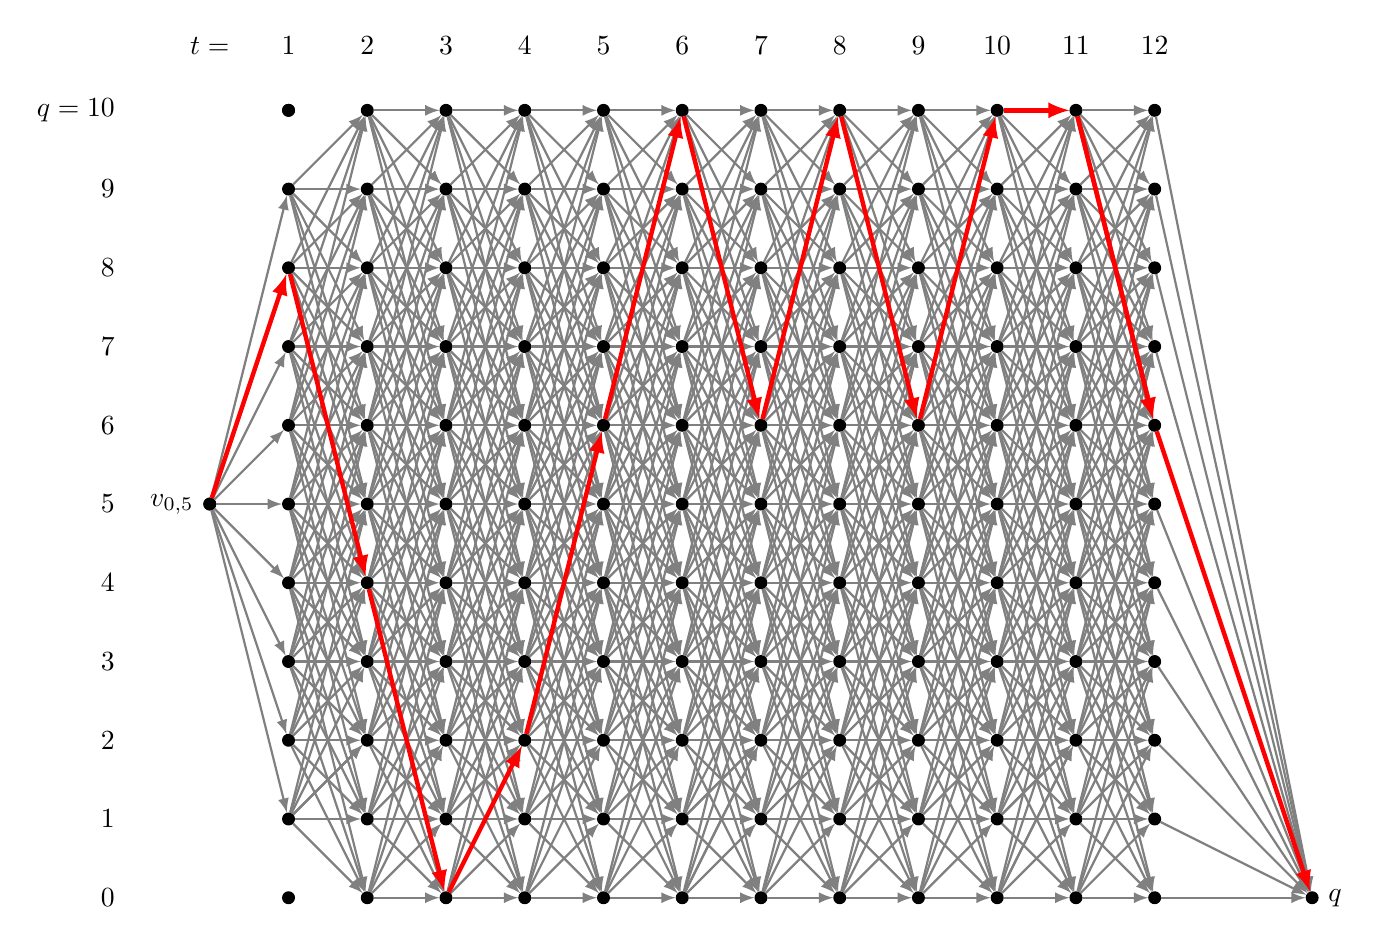
\begin{tikzpicture}

       \tikzset{enclosed/.style={draw, circle, inner sep=0pt, minimum size=.15cm, fill=black}}
%% Vertices
      	\node[enclosed, label={left: $v_{0,5}$}] (vstart) at (-1,5) {};
      	\node[enclosed, label={[label distance=5.5cm]90: $t=$}] (vstart) at (-1,5) {};
      	\node[enclosed, label={[label distance=2cm]180: $0$}] (v00) at (0,0) {};
    		\node[enclosed, label={[label distance=2cm]180: $1$}] (v01) at (0,1) {};
  	    \node[enclosed, label={[label distance=2cm]180: $2$}] (v02) at (0,2) {};
     	\node[enclosed, label={[label distance=2cm]180: $3$}] (v03) at (0,3) {};
     	\node[enclosed, label={[label distance=2cm]180: $4$}] (v04) at (0,4) {};
     	\node[enclosed, label={[label distance=2cm]180: $5$}] (v05) at (0,5) {};
     	\node[enclosed, label={[label distance=2cm]180: $6$}] (v06) at (0,6) {};
     	\node[enclosed, label={[label distance=2cm]180: $7$}] (v07) at (0,7) {};
     	\node[enclosed, label={[label distance=2cm]180: $8$}] (v08) at (0,8) {};
     	\node[enclosed, label={[label distance=2cm]180: $9$}] (v09) at (0,9) {};
     	\node[enclosed, label={[label distance=2cm]180: $q=10$}] (v010) at (0,10) {};
     	\node[enclosed, label={[label distance=0.5cm]90: $1$}] (v010) at (0,10) {};
      	\node[enclosed, label={above: }] (v10) at (1,0) {};
  	    \node[enclosed, label={below: }] (v11) at (1,1) {};
  	    \node[enclosed, label={below: }] (v12) at (1,2) {};
     	\node[enclosed, label={above:  }] (v13) at (1,3) {};
     	\node[enclosed, label={below: }] (v14) at (1,4) {};
     	 \node[enclosed, label={below:}] (v15) at (1,5) {};
     	\node[enclosed, label={above: }] (v16) at (1,6) {};
     	\node[enclosed, label={below: }] (v17) at (1,7) {};
     	\node[enclosed, label={above: }] (v18) at (1,8) {};
     	\node[enclosed, label={below:  }] (v19) at (1,9) {};
     	\node[enclosed, label={[label distance=0.5cm]90: $2$}] (v110) at (1,10) {};
     	\node[enclosed, label={below: }] (v20) at (2,0) {};
    		\node[enclosed, label={below: }] (v21) at (2,1) {};
  	    \node[enclosed, label={above: }] (v22) at (2,2) {};
     	\node[enclosed, label={below: }] (v23) at (2,3) {};
     	\node[enclosed, label={below:  }] (v24) at (2,4) {};
     	\node[enclosed, label={above: }] (v25) at (2,5) {};
     	\node[enclosed, label={below: }] (v26) at (2,6) {};
     	\node[enclosed, label={below: }] (v27) at (2,7) {};
     	\node[enclosed, label={above: }] (v28) at (2,8) {};
     	\node[enclosed, label={below:  }] (v29) at (2,9) {};
     	\node[enclosed, label={[label distance=0.5cm]90: $3$}] (v210) at (2,10) {};
      	\node[enclosed, label={above: }] (v30) at (3,0) {};
  	    \node[enclosed, label={below: }] (v31) at (3,1) {};
  	    \node[enclosed, label={below: }] (v32) at (3,2) {};
     	\node[enclosed, label={above:  }] (v33) at (3,3) {};
     	\node[enclosed, label={below: }] (v34) at (3,4) {};
     	 \node[enclosed, label={below:}] (v35) at (3,5) {};
     	\node[enclosed, label={above: }] (v36) at (3,6) {};
     	\node[enclosed, label={below: }] (v37) at (3,7) {};
     	\node[enclosed, label={above: }] (v38) at (3,8) {};
     	\node[enclosed, label={below:  }] (v39) at (3,9) {};
     	\node[enclosed, label={[label distance=0.5cm]90: $4$}] (v310) at (3,10) {};
     	 \node[enclosed, label={below: }] (v40) at (4,0) {};
    		\node[enclosed, label={below: }] (v41) at (4,1) {};
  	    \node[enclosed, label={above: }] (v42) at (4,2) {};
     	\node[enclosed, label={below: }] (v43) at (4,3) {};
     	\node[enclosed, label={below:  }] (v44) at (4,4) {};
     	\node[enclosed, label={above: }] (v45) at (4,5) {};
     	\node[enclosed, label={below: }] (v46) at (4,6) {};
     	\node[enclosed, label={below: }] (v47) at (4,7) {};
     	\node[enclosed, label={above: }] (v48) at (4,8) {};
     	\node[enclosed, label={below:  }] (v49) at (4,9) {};
     	\node[enclosed, label={[label distance=0.5cm]90: $5$}] (v410) at (4,10) {};
      	\node[enclosed, label={above: }] (v50) at (5,0) {};
  	    \node[enclosed, label={below: }] (v51) at (5,1) {};
  	    \node[enclosed, label={below: }] (v52) at (5,2) {};
     	\node[enclosed, label={above:  }] (v53) at (5,3) {};
     	\node[enclosed, label={below: }] (v54) at (5,4) {};
     	 \node[enclosed, label={below:}] (v55) at (5,5) {};
     	\node[enclosed, label={above: }] (v56) at (5,6) {};
     	\node[enclosed, label={below: }] (v57) at (5,7) {};
     	\node[enclosed, label={above: }] (v58) at (5,8) {};
     	\node[enclosed, label={below:  }] (v59) at (5,9) {};
     	\node[enclosed, label={[label distance=0.5cm]90: $6$}] (v510) at (5,10) {};
     	\node[enclosed, label={below: }] (v60) at (6,0) {};
    		\node[enclosed, label={below: }] (v61) at (6,1) {};
  	    \node[enclosed, label={above: }] (v62) at (6,2) {};
     	\node[enclosed, label={below: }] (v63) at (6,3) {};
     	\node[enclosed, label={below:  }] (v64) at (6,4) {};
     	\node[enclosed, label={above: }] (v65) at (6,5) {};
     	\node[enclosed, label={below: }] (v66) at (6,6) {};
     	\node[enclosed, label={below: }] (v67) at (6,7) {};
     	\node[enclosed, label={above: }] (v68) at (6,8) {};
     	\node[enclosed, label={below:  }] (v69) at (6,9) {};
     	\node[enclosed, label={[label distance=0.5cm]90: $7$}] (v610) at (6,10) {};
      	\node[enclosed, label={above: }] (v70) at (7,0) {};
  	    \node[enclosed, label={below: }] (v71) at (7,1) {};
  	    \node[enclosed, label={below: }] (v72) at (7,2) {};
     	\node[enclosed, label={above:  }] (v73) at (7,3) {};
     	\node[enclosed, label={below: }] (v74) at (7,4) {};
     	 \node[enclosed, label={below:}] (v75) at (7,5) {};
     	\node[enclosed, label={above: }] (v76) at (7,6) {};
     	\node[enclosed, label={below: }] (v77) at (7,7) {};
     	\node[enclosed, label={above: }] (v78) at (7,8) {};
     	\node[enclosed, label={below:  }] (v79) at (7,9) {};
     	\node[enclosed, label={[label distance=0.5cm]90: $8$}] (v710) at (7,10) {};
     	\node[enclosed, label={above: }] (v80) at (8,0) {};
  	    \node[enclosed, label={below: }] (v81) at (8,1) {};
  	    \node[enclosed, label={below: }] (v82) at (8,2) {};
     	\node[enclosed, label={above:  }] (v83) at (8,3) {};
     	\node[enclosed, label={below: }] (v84) at (8,4) {};
     	 \node[enclosed, label={below:}] (v85) at (8,5) {};
     	\node[enclosed, label={above: }] (v86) at (8,6) {};
     	\node[enclosed, label={below: }] (v87) at (8,7) {};
     	\node[enclosed, label={above: }] (v88) at (8,8) {};
     	\node[enclosed, label={below:  }] (v89) at (8,9) {};
     	\node[enclosed, label={[label distance=0.5cm]90: $9$}] (v810) at (8,10) {};
     	\node[enclosed, label={below: }] (v90) at (9,0) {};
    		\node[enclosed, label={below: }] (v91) at (9,1) {};
  	    \node[enclosed, label={above: }] (v92) at (9,2) {};
     	\node[enclosed, label={below: }] (v93) at (9,3) {};
     	\node[enclosed, label={below:  }] (v94) at (9,4) {};
     	\node[enclosed, label={above: }] (v95) at (9,5) {};
     	\node[enclosed, label={below: }] (v96) at (9,6) {};
     	\node[enclosed, label={below: }] (v97) at (9,7) {};
     	\node[enclosed, label={above: }] (v98) at (9,8) {};
     	\node[enclosed, label={below:  }] (v99) at (9,9) {};
     	\node[enclosed, label={[label distance=0.5cm]90: $10$}] (v910) at (9,10) {};
      	\node[enclosed, label={above: }] (v100) at (10,0) {};
  	    \node[enclosed, label={below: }] (v101) at (10,1) {};
  	    \node[enclosed, label={below: }] (v102) at (10,2) {};
     	\node[enclosed, label={above:  }] (v103) at (10,3) {};
     	\node[enclosed, label={below: }] (v104) at (10,4) {};
     	 \node[enclosed, label={below:}] (v105) at (10,5) {};
     	\node[enclosed, label={above: }] (v106) at (10,6) {};
     	\node[enclosed, label={below: }] (v107) at (10,7) {};
     	\node[enclosed, label={above: }] (v108) at (10,8) {};
     	\node[enclosed, label={below:  }] (v109) at (10,9) {};
     	\node[enclosed, label={[label distance=0.5cm]90: $11$}] (v1010) at (10,10) {};
     	\node[enclosed, label={above: }] (v1100) at (11,0) {};
  	    \node[enclosed, label={below: }] (v111) at (11,1) {};
  	    \node[enclosed, label={below: }] (v112) at (11,2) {};
     	\node[enclosed, label={above:  }] (v113) at (11,3) {};
     	\node[enclosed, label={below: }] (v114) at (11,4) {};
     	 \node[enclosed, label={below:}] (v115) at (11,5) {};
     	\node[enclosed, label={above: }] (v116) at (11,6) {};
     	\node[enclosed, label={below: }] (v117) at (11,7) {};
     	\node[enclosed, label={above: }] (v118) at (11,8) {};
     	\node[enclosed, label={below:  }] (v119) at (11,9) {};
     	\node[enclosed, label={[label distance=0.5cm]90: $12$}] (v1110) at (11,10) {};
     	\node[enclosed, label={right: $q_{\slut}$ }] (v120) at (13,0) {};
     	
%Edges
		\path[gray,->,>=latex,thick] (vstart) edge node[midway, sloped, above] {} (v01);
		\path[gray,->,>=latex,thick] (vstart) edge node[midway, sloped, below] {} (v02);
		\path[gray,->,>=latex,thick] (vstart) edge node[midway, sloped, below] {} (v03);
		\path[gray,->,>=latex,thick] (vstart) edge node[midway, sloped, above] {} (v04);
		\path[gray,->,>=latex,thick] (vstart) edge node[midway, above] {} (v05);
		\path[gray,->,>=latex,thick] (vstart) edge node[near end, sloped, below] {} (v06);
		\path[gray,->,>=latex,thick] (vstart) edge node[midway, sloped, below] {} (v07);
		\path[gray,->,>=latex,thick] (vstart) edge node[near end, sloped, below] {} (v09);
		\path[gray,->,>=latex,thick] (v01) edge node[midway, sloped, below] {} (v10);
		\path[gray,->,>=latex,thick] (v01) edge node[midway, sloped, above] {} (v11);
		\path[gray,->,>=latex,thick] (v01) edge node[midway, above] {} (v12);
		\path[gray,->,>=latex,thick] (v01) edge node[near end, sloped, below] {} (v12);
		\path[gray,->,>=latex,thick] (v01) edge node[midway, sloped, below] {} (v13);
		\path[gray,->,>=latex,thick] (v01) edge node[midway, above] {} (v14);
		\path[gray,->,>=latex,thick] (v01) edge node[near end, sloped, below] {} (v15);
		\path[gray,->,>=latex,thick] (v02) edge node[midway, sloped, below] {} (v10);
		\path[gray,->,>=latex,thick] (v02) edge node[midway, sloped, above] {} (v11);
		\path[gray,->,>=latex,thick] (v02) edge node[midway, above] {} (v12);
		\path[gray,->,>=latex,thick] (v02) edge node[near end, sloped, below] {} (v13);
		\path[gray,->,>=latex,thick] (v02) edge node[midway, sloped, below] {} (v14);
		\path[gray,->,>=latex,thick] (v02) edge node[midway, above] {} (v15);
		\path[gray,->,>=latex,thick] (v02) edge node[near end, sloped, below] {} (v16);
		\path[gray,->,>=latex,thick] (v03) edge node[midway, sloped, below] {} (v10);
		\path[gray,->,>=latex,thick] (v03) edge node[midway, sloped, above] {} (v11);
		\path[gray,->,>=latex,thick] (v03) edge node[midway, above] {} (v12);
		\path[gray,->,>=latex,thick] (v03) edge node[near end, sloped, below] {} (v13);
		\path[gray,->,>=latex,thick] (v03) edge node[midway, sloped, below] {} (v14);
		\path[gray,->,>=latex,thick] (v03) edge node[midway, above] {} (v15);
		\path[gray,->,>=latex,thick] (v03) edge node[near end, sloped, below] {} (v16);
		\path[gray,->,>=latex,thick] (v03) edge node[midway, sloped, below] {} (v17);
		\path[gray,->,>=latex,thick] (v04) edge node[midway, sloped, below] {} (v10);
		\path[gray,->,>=latex,thick] (v04) edge node[midway, sloped, above] {} (v11);
		\path[gray,->,>=latex,thick] (v04) edge node[midway, above] {} (v12);
		\path[gray,->,>=latex,thick] (v04) edge node[near end, sloped, below] {} (v13);
		\path[gray,->,>=latex,thick] (v04) edge node[midway, sloped, below] {} (v14);
		\path[gray,->,>=latex,thick] (v04) edge node[midway, above] {} (v15);
		\path[gray,->,>=latex,thick] (v04) edge node[near end, sloped, below] {} (v16);
		\path[gray,->,>=latex,thick] (v04) edge node[midway, sloped, below] {} (v17);
		\path[gray,->,>=latex,thick] (v04) edge node[midway, sloped, above] {} (v18);
		\path[gray,->,>=latex,thick] (v05) edge node[midway, sloped, above] {} (v11);
		\path[gray,->,>=latex,thick] (v05) edge node[midway, above] {} (v12);
		\path[gray,->,>=latex,thick] (v05) edge node[near end, sloped, below] {} (v13);
		\path[gray,->,>=latex,thick] (v05) edge node[midway, sloped, below] {} (v14);
		\path[gray,->,>=latex,thick] (v05) edge node[midway, above] {} (v15);
		\path[gray,->,>=latex,thick] (v05) edge node[near end, sloped, below] {} (v16);
		\path[gray,->,>=latex,thick] (v05) edge node[midway, sloped, below] {} (v17);
		\path[gray,->,>=latex,thick] (v05) edge node[midway, sloped, above] {} (v18);
		\path[gray,->,>=latex,thick] (v05) edge node[midway, sloped, above] {} (v19);
		\path[gray,->,>=latex,thick] (v06) edge node[midway, above] {} (v12);
		\path[gray,->,>=latex,thick] (v06) edge node[near end, sloped, below] {} (v13);
		\path[gray,->,>=latex,thick] (v06) edge node[midway, sloped, below] {} (v14);
		\path[gray,->,>=latex,thick] (v06) edge node[midway, above] {} (v15);
		\path[gray,->,>=latex,thick] (v06) edge node[near end, sloped, below] {} (v16);
		\path[gray,->,>=latex,thick] (v06) edge node[midway, sloped, below] {} (v17);
		\path[gray,->,>=latex,thick] (v06) edge node[midway, sloped, above] {} (v18);
		\path[gray,->,>=latex,thick] (v06) edge node[midway, sloped, above] {} (v19);
		\path[gray,->,>=latex,thick] (v06) edge node[midway, sloped, above] {} (v110);
		\path[gray,->,>=latex,thick] (v07) edge node[near end, sloped, below] {} (v13);
		\path[gray,->,>=latex,thick] (v07) edge node[midway, sloped, below] {} (v14);
		\path[gray,->,>=latex,thick] (v07) edge node[midway, above] {} (v15);
		\path[gray,->,>=latex,thick] (v07) edge node[near end, sloped, below] {} (v16);
		\path[gray,->,>=latex,thick] (v07) edge node[midway, sloped, below] {} (v17);
		\path[gray,->,>=latex,thick] (v07) edge node[midway, sloped, above] {} (v18);
		\path[gray,->,>=latex,thick] (v07) edge node[midway, sloped, above] {} (v19);
		\path[gray,->,>=latex,thick] (v07) edge node[midway, sloped, above] {} (v110);
		\path[gray,->,>=latex,thick] (v08) edge node[midway, above] {} (v15);
		\path[gray,->,>=latex,thick] (v08) edge node[near end, sloped, below] {} (v16);
		\path[gray,->,>=latex,thick] (v08) edge node[midway, sloped, below] {} (v17);
		\path[gray,->,>=latex,thick] (v08) edge node[midway, sloped, above] {} (v18);
		\path[gray,->,>=latex,thick] (v08) edge node[midway, sloped, above] {} (v19);
		\path[gray,->,>=latex,thick] (v08) edge node[midway, sloped, above] {} (v110);
		\path[gray,->,>=latex,thick] (v09) edge node[midway, above] {} (v15);
		\path[gray,->,>=latex,thick] (v09) edge node[near end, sloped, below] {} (v16);
		\path[gray,->,>=latex,thick] (v09) edge node[midway, sloped, below] {} (v17);
		\path[gray,->,>=latex,thick] (v09) edge node[midway, sloped, above] {} (v18);
		\path[gray,->,>=latex,thick] (v09) edge node[midway, sloped, above] {} (v19);
		\path[gray,->,>=latex,thick] (v09) edge node[midway, sloped, above] {} (v110);
		\path[gray,->,>=latex,thick] (v10) edge node[midway, sloped, below] {} (v20);
		\path[gray,->,>=latex,thick] (v10) edge node[midway, sloped, above] {} (v21);
		\path[gray,->,>=latex,thick] (v10) edge node[midway, above] {} (v22);
		\path[gray,->,>=latex,thick] (v10) edge node[midway, sloped, below] {} (v23);
		\path[gray,->,>=latex,thick] (v10) edge node[midway, above] {} (v24);
		\path[gray,->,>=latex,thick] (v11) edge node[midway, sloped, below] {} (v20);
		\path[gray,->,>=latex,thick] (v11) edge node[midway, sloped, above] {} (v21);
		\path[gray,->,>=latex,thick] (v11) edge node[midway, above] {} (v22);
		\path[gray,->,>=latex,thick] (v11) edge node[midway, sloped, below] {} (v23);
		\path[gray,->,>=latex,thick] (v11) edge node[midway, above] {} (v24);
		\path[gray,->,>=latex,thick] (v11) edge node[near end, sloped, below] {} (v25);
		\path[gray,->,>=latex,thick] (v12) edge node[midway, sloped, below] {} (v20);
		\path[gray,->,>=latex,thick] (v12) edge node[midway, sloped, above] {} (v21);
		\path[gray,->,>=latex,thick] (v12) edge node[midway, above] {} (v22);
		\path[gray,->,>=latex,thick] (v12) edge node[near end, sloped, below] {} (v23);
		\path[gray,->,>=latex,thick] (v12) edge node[midway, sloped, below] {} (v24);
		\path[gray,->,>=latex,thick] (v12) edge node[midway, above] {} (v25);
		\path[gray,->,>=latex,thick] (v12) edge node[near end, sloped, below] {} (v26);
		\path[gray,->,>=latex,thick] (v13) edge node[midway, sloped, below] {} (v20);
		\path[gray,->,>=latex,thick] (v13) edge node[midway, sloped, above] {} (v21);
		\path[gray,->,>=latex,thick] (v13) edge node[midway, above] {} (v22);
		\path[gray,->,>=latex,thick] (v13) edge node[near end, sloped, below] {} (v23);
		\path[gray,->,>=latex,thick] (v13) edge node[midway, sloped, below] {} (v24);
		\path[gray,->,>=latex,thick] (v13) edge node[midway, above] {} (v25);
		\path[gray,->,>=latex,thick] (v13) edge node[near end, sloped, below] {} (v26);
		\path[gray,->,>=latex,thick] (v13) edge node[midway, sloped, below] {} (v27);
		\path[gray,->,>=latex,thick] (v14) edge node[midway, sloped, above] {} (v21);
		\path[gray,->,>=latex,thick] (v14) edge node[midway, above] {} (v22);
		\path[gray,->,>=latex,thick] (v14) edge node[near end, sloped, below] {} (v23);
		\path[gray,->,>=latex,thick] (v14) edge node[midway, sloped, below] {} (v24);
		\path[gray,->,>=latex,thick] (v14) edge node[midway, above] {} (v25);
		\path[gray,->,>=latex,thick] (v14) edge node[near end, sloped, below] {} (v26);
		\path[gray,->,>=latex,thick] (v14) edge node[midway, sloped, below] {} (v27);
		\path[gray,->,>=latex,thick] (v14) edge node[midway, sloped, above] {} (v28);
		\path[gray,->,>=latex,thick] (v15) edge node[midway, sloped, above] {} (v21);
		\path[gray,->,>=latex,thick] (v15) edge node[midway, above] {} (v22);
		\path[gray,->,>=latex,thick] (v15) edge node[near end, sloped, below] {} (v23);
		\path[gray,->,>=latex,thick] (v15) edge node[midway, sloped, below] {} (v24);
		\path[gray,->,>=latex,thick] (v15) edge node[midway, above] {} (v25);
		\path[gray,->,>=latex,thick] (v15) edge node[near end, sloped, below] {} (v26);
		\path[gray,->,>=latex,thick] (v15) edge node[midway, sloped, below] {} (v27);
		\path[gray,->,>=latex,thick] (v15) edge node[midway, sloped, above] {} (v28);
		\path[gray,->,>=latex,thick] (v15) edge node[midway, sloped, above] {} (v29);
		\path[gray,->,>=latex,thick] (v16) edge node[midway, above] {} (v22);
		\path[gray,->,>=latex,thick] (v16) edge node[near end, sloped, below] {} (v23);
		\path[gray,->,>=latex,thick] (v16) edge node[midway, sloped, below] {} (v24);
		\path[gray,->,>=latex,thick] (v16) edge node[midway, above] {} (v25);
		\path[gray,->,>=latex,thick] (v16) edge node[near end, sloped, below] {} (v26);
		\path[gray,->,>=latex,thick] (v16) edge node[midway, sloped, below] {} (v27);
		\path[gray,->,>=latex,thick] (v16) edge node[midway, sloped, above] {} (v28);
		\path[gray,->,>=latex,thick] (v16) edge node[midway, sloped, above] {} (v29);
		\path[gray,->,>=latex,thick] (v16) edge node[midway, sloped, above] {} (v210);
		\path[gray,->,>=latex,thick] (v17) edge node[near end, sloped, below] {} (v23);
		\path[gray,->,>=latex,thick] (v17) edge node[midway, sloped, below] {} (v24);
		\path[gray,->,>=latex,thick] (v17) edge node[midway, above] {} (v25);
		\path[gray,->,>=latex,thick] (v17) edge node[near end, sloped, below] {} (v26);
		\path[gray,->,>=latex,thick] (v17) edge node[midway, sloped, below] {} (v27);
		\path[gray,->,>=latex,thick] (v17) edge node[midway, sloped, above] {} (v28);
		\path[gray,->,>=latex,thick] (v17) edge node[midway, sloped, above] {} (v29);
		\path[gray,->,>=latex,thick] (v17) edge node[midway, sloped, above] {} (v210);
		\path[gray,->,>=latex,thick] (v18) edge node[midway, sloped, below] {} (v24);
		\path[gray,->,>=latex,thick] (v18) edge node[midway, above] {} (v25);
		\path[gray,->,>=latex,thick] (v18) edge node[near end, sloped, below] {} (v26);
		\path[gray,->,>=latex,thick] (v18) edge node[midway, sloped, below] {} (v27);
		\path[gray,->,>=latex,thick] (v18) edge node[midway, sloped, above] {} (v28);
		\path[gray,->,>=latex,thick] (v18) edge node[midway, sloped, above] {} (v29);
		\path[gray,->,>=latex,thick] (v18) edge node[midway, sloped, above] {} (v210);
		\path[gray,->,>=latex,thick] (v19) edge node[midway, above] {} (v25);
		\path[gray,->,>=latex,thick] (v19) edge node[near end, sloped, below] {} (v26);
		\path[gray,->,>=latex,thick] (v19) edge node[midway, sloped, below] {} (v27);
		\path[gray,->,>=latex,thick] (v19) edge node[midway, sloped, above] {} (v28);
		\path[gray,->,>=latex,thick] (v19) edge node[midway, sloped, above] {} (v29);
		\path[gray,->,>=latex,thick] (v19) edge node[midway, sloped, above] {} (v210);
		\path[gray,->,>=latex,thick] (v110) edge node[near end, sloped, below] {} (v26);
		\path[gray,->,>=latex,thick] (v110) edge node[midway, sloped, below] {} (v27);
		\path[gray,->,>=latex,thick] (v110) edge node[midway, sloped, above] {} (v28);
		\path[gray,->,>=latex,thick] (v110) edge node[midway, sloped, above] {} (v29);
		\path[gray,->,>=latex,thick] (v110) edge node[midway, sloped, above] {} (v210);
		\path[gray,->,>=latex,thick] (v20) edge node[midway, sloped, below] {} (v30);
		\path[gray,->,>=latex,thick] (v20) edge node[midway, sloped, above] {} (v31);
		\path[gray,->,>=latex,thick] (v20) edge node[near end, sloped, below] {} (v32);
		\path[gray,->,>=latex,thick] (v20) edge node[midway, sloped, below] {} (v33);
		\path[gray,->,>=latex,thick] (v20) edge node[midway, above] {} (v34);
		\path[gray,->,>=latex,thick] (v21) edge node[midway, sloped, below] {} (v30);
		\path[gray,->,>=latex,thick] (v21) edge node[midway, sloped, above] {} (v31);
		\path[gray,->,>=latex,thick] (v21) edge node[midway, above] {} (v32);
		\path[gray,->,>=latex,thick] (v21) edge node[near end, sloped, below] {} (v32);
		\path[gray,->,>=latex,thick] (v21) edge node[midway, sloped, below] {} (v33);
		\path[gray,->,>=latex,thick] (v21) edge node[midway, above] {} (v34);
		\path[gray,->,>=latex,thick] (v21) edge node[near end, sloped, below] {} (v35);
		\path[gray,->,>=latex,thick] (v22) edge node[midway, sloped, below] {} (v30);
		\path[gray,->,>=latex,thick] (v22) edge node[midway, sloped, above] {} (v31);
		\path[gray,->,>=latex,thick] (v22) edge node[midway, above] {} (v32);
		\path[gray,->,>=latex,thick] (v22) edge node[near end, sloped, below] {} (v33);
		\path[gray,->,>=latex,thick] (v22) edge node[midway, sloped, below] {} (v34);
		\path[gray,->,>=latex,thick] (v22) edge node[midway, above] {} (v35);
		\path[gray,->,>=latex,thick] (v22) edge node[near end, sloped, below] {} (v36);
		\path[gray,->,>=latex,thick] (v23) edge node[midway, sloped, below] {} (v30);
		\path[gray,->,>=latex,thick] (v23) edge node[midway, sloped, above] {} (v31);
		\path[gray,->,>=latex,thick] (v23) edge node[midway, above] {} (v32);
		\path[gray,->,>=latex,thick] (v23) edge node[near end, sloped, below] {} (v33);
		\path[gray,->,>=latex,thick] (v23) edge node[midway, sloped, below] {} (v34);
		\path[gray,->,>=latex,thick] (v23) edge node[midway, above] {} (v35);
		\path[gray,->,>=latex,thick] (v23) edge node[near end, sloped, below] {} (v36);
		\path[gray,->,>=latex,thick] (v23) edge node[midway, sloped, below] {} (v37);
		\path[gray,->,>=latex,thick] (v24) edge node[midway, sloped, below] {} (v30);
		\path[gray,->,>=latex,thick] (v24) edge node[midway, sloped, above] {} (v31);
		\path[gray,->,>=latex,thick] (v24) edge node[midway, above] {} (v32);
		\path[gray,->,>=latex,thick] (v24) edge node[near end, sloped, below] {} (v33);
		\path[gray,->,>=latex,thick] (v24) edge node[midway, sloped, below] {} (v34);
		\path[gray,->,>=latex,thick] (v24) edge node[midway, above] {} (v35);
		\path[gray,->,>=latex,thick] (v24) edge node[near end, sloped, below] {} (v36);
		\path[gray,->,>=latex,thick] (v24) edge node[midway, sloped, below] {} (v37);
		\path[gray,->,>=latex,thick] (v24) edge node[midway, sloped, above] {} (v38);
		\path[gray,->,>=latex,thick] (v25) edge node[midway, sloped, above] {} (v31);
		\path[gray,->,>=latex,thick] (v25) edge node[midway, above] {} (v32);
		\path[gray,->,>=latex,thick] (v25) edge node[near end, sloped, below] {} (v33);
		\path[gray,->,>=latex,thick] (v25) edge node[midway, sloped, below] {} (v34);
		\path[gray,->,>=latex,thick] (v25) edge node[midway, above] {} (v35);
		\path[gray,->,>=latex,thick] (v25) edge node[near end, sloped, below] {} (v36);
		\path[gray,->,>=latex,thick] (v25) edge node[midway, sloped, below] {} (v37);
		\path[gray,->,>=latex,thick] (v25) edge node[midway, sloped, above] {} (v38);
		\path[gray,->,>=latex,thick] (v25) edge node[midway, sloped, above] {} (v39);
		\path[gray,->,>=latex,thick] (v26) edge node[midway, above] {} (v32);
		\path[gray,->,>=latex,thick] (v26) edge node[near end, sloped, below] {} (v33);
		\path[gray,->,>=latex,thick] (v26) edge node[midway, sloped, below] {} (v34);
		\path[gray,->,>=latex,thick] (v26) edge node[midway, above] {} (v35);
		\path[gray,->,>=latex,thick] (v26) edge node[near end, sloped, below] {} (v36);
		\path[gray,->,>=latex,thick] (v26) edge node[midway, sloped, below] {} (v37);
		\path[gray,->,>=latex,thick] (v26) edge node[midway, sloped, above] {} (v38);
		\path[gray,->,>=latex,thick] (v26) edge node[midway, sloped, above] {} (v39);
		\path[gray,->,>=latex,thick] (v26) edge node[midway, sloped, above] {} (v310);
		\path[gray,->,>=latex,thick] (v27) edge node[near end, sloped, below] {} (v33);
		\path[gray,->,>=latex,thick] (v27) edge node[midway, sloped, below] {} (v34);
		\path[gray,->,>=latex,thick] (v27) edge node[midway, above] {} (v35);
		\path[gray,->,>=latex,thick] (v27) edge node[near end, sloped, below] {} (v36);
		\path[gray,->,>=latex,thick] (v27) edge node[midway, sloped, below] {} (v37);
		\path[gray,->,>=latex,thick] (v27) edge node[midway, sloped, above] {} (v38);
		\path[gray,->,>=latex,thick] (v27) edge node[midway, sloped, above] {} (v39);
		\path[gray,->,>=latex,thick] (v27) edge node[midway, sloped, above] {} (v310);
		\path[gray,->,>=latex,thick] (v28) edge node[midway, sloped, below] {} (v34);
		\path[gray,->,>=latex,thick] (v28) edge node[midway, above] {} (v35);
		\path[gray,->,>=latex,thick] (v28) edge node[near end, sloped, below] {} (v36);
		\path[gray,->,>=latex,thick] (v28) edge node[midway, sloped, below] {} (v37);
		\path[gray,->,>=latex,thick] (v28) edge node[midway, sloped, above] {} (v38);
		\path[gray,->,>=latex,thick] (v28) edge node[midway, sloped, above] {} (v39);
		\path[gray,->,>=latex,thick] (v28) edge node[midway, sloped, above] {} (v310);
		\path[gray,->,>=latex,thick] (v29) edge node[midway, above] {} (v35);
		\path[gray,->,>=latex,thick] (v29) edge node[near end, sloped, below] {} (v36);
		\path[gray,->,>=latex,thick] (v29) edge node[midway, sloped, below] {} (v37);
		\path[gray,->,>=latex,thick] (v29) edge node[midway, sloped, above] {} (v38);
		\path[gray,->,>=latex,thick] (v29) edge node[midway, sloped, above] {} (v39);
		\path[gray,->,>=latex,thick] (v29) edge node[midway, sloped, above] {} (v310);
		\path[gray,->,>=latex,thick] (v210) edge node[near end, sloped, below] {} (v36);
		\path[gray,->,>=latex,thick] (v210) edge node[midway, sloped, below] {} (v37);
		\path[gray,->,>=latex,thick] (v210) edge node[midway, sloped, above] {} (v38);
		\path[gray,->,>=latex,thick] (v210) edge node[midway, sloped, above] {} (v39);
		\path[gray,->,>=latex,thick] (v210) edge node[midway, sloped, above] {} (v310);
		\path[gray,->,>=latex,thick] (v30) edge node[midway, sloped, below] {} (v40);
		\path[gray,->,>=latex,thick] (v30) edge node[midway, sloped, above] {} (v41);
		\path[gray,->,>=latex,thick] (v30) edge node[midway, above] {} (v42);
		\path[gray,->,>=latex,thick] (v30) edge node[midway, sloped, below] {} (v43);
		\path[gray,->,>=latex,thick] (v30) edge node[midway, above] {} (v44);
		\path[gray,->,>=latex,thick] (v31) edge node[midway, sloped, below] {} (v40);
		\path[gray,->,>=latex,thick] (v31) edge node[midway, sloped, above] {} (v41);
		\path[gray,->,>=latex,thick] (v31) edge node[midway, above] {} (v42);
		\path[gray,->,>=latex,thick] (v31) edge node[midway, sloped, below] {} (v43);
		\path[gray,->,>=latex,thick] (v31) edge node[midway, above] {} (v44);
		\path[gray,->,>=latex,thick] (v31) edge node[near end, sloped, below] {} (v45);
		\path[gray,->,>=latex,thick] (v32) edge node[midway, sloped, below] {} (v40);
		\path[gray,->,>=latex,thick] (v32) edge node[midway, sloped, above] {} (v41);
		\path[gray,->,>=latex,thick] (v32) edge node[midway, above] {} (v42);
		\path[gray,->,>=latex,thick] (v32) edge node[near end, sloped, below] {} (v43);
		\path[gray,->,>=latex,thick] (v32) edge node[midway, sloped, below] {} (v44);
		\path[gray,->,>=latex,thick] (v32) edge node[midway, above] {} (v45);
		\path[gray,->,>=latex,thick] (v33) edge node[midway, sloped, below] {} (v40);
		\path[gray,->,>=latex,thick] (v33) edge node[midway, sloped, above] {} (v41);
		\path[gray,->,>=latex,thick] (v33) edge node[midway, above] {} (v42);
		\path[gray,->,>=latex,thick] (v33) edge node[near end, sloped, below] {} (v43);
		\path[gray,->,>=latex,thick] (v33) edge node[midway, sloped, below] {} (v44);
		\path[gray,->,>=latex,thick] (v33) edge node[midway, above] {} (v45);
		\path[gray,->,>=latex,thick] (v33) edge node[near end, sloped, below] {} (v46);
		\path[gray,->,>=latex,thick] (v33) edge node[midway, sloped, below] {} (v47);
		\path[gray,->,>=latex,thick] (v34) edge node[midway, sloped, below] {} (v40);
		\path[gray,->,>=latex,thick] (v34) edge node[midway, sloped, above] {} (v41);
		\path[gray,->,>=latex,thick] (v34) edge node[midway, above] {} (v42);
		\path[gray,->,>=latex,thick] (v34) edge node[near end, sloped, below] {} (v43);
		\path[gray,->,>=latex,thick] (v34) edge node[midway, sloped, below] {} (v44);
		\path[gray,->,>=latex,thick] (v34) edge node[midway, above] {} (v45);
		\path[gray,->,>=latex,thick] (v34) edge node[near end, sloped, below] {} (v46);
		\path[gray,->,>=latex,thick] (v34) edge node[midway, sloped, below] {} (v47);
		\path[gray,->,>=latex,thick] (v34) edge node[midway, sloped, above] {} (v48);
		\path[gray,->,>=latex,thick] (v35) edge node[midway, sloped, above] {} (v41);
		\path[gray,->,>=latex,thick] (v35) edge node[midway, above] {} (v42);
		\path[gray,->,>=latex,thick] (v35) edge node[near end, sloped, below] {} (v43);
		\path[gray,->,>=latex,thick] (v35) edge node[midway, sloped, below] {} (v44);
		\path[gray,->,>=latex,thick] (v35) edge node[midway, above] {} (v45);
		\path[gray,->,>=latex,thick] (v35) edge node[near end, sloped, below] {} (v46);
		\path[gray,->,>=latex,thick] (v35) edge node[midway, sloped, below] {} (v47);
		\path[gray,->,>=latex,thick] (v35) edge node[midway, sloped, above] {} (v48);
		\path[gray,->,>=latex,thick] (v35) edge node[midway, sloped, above] {} (v49);
		\path[gray,->,>=latex,thick] (v36) edge node[midway, above] {} (v42);
		\path[gray,->,>=latex,thick] (v36) edge node[near end, sloped, below] {} (v43);
		\path[gray,->,>=latex,thick] (v36) edge node[midway, sloped, below] {} (v44);
		\path[gray,->,>=latex,thick] (v36) edge node[midway, above] {} (v45);
		\path[gray,->,>=latex,thick] (v36) edge node[near end, sloped, below] {} (v46);
		\path[gray,->,>=latex,thick] (v36) edge node[midway, sloped, below] {} (v47);
		\path[gray,->,>=latex,thick] (v36) edge node[midway, sloped, above] {} (v48);
		\path[gray,->,>=latex,thick] (v36) edge node[midway, sloped, above] {} (v49);
		\path[gray,->,>=latex,thick] (v36) edge node[midway, sloped, above] {} (v410);
		\path[gray,->,>=latex,thick] (v37) edge node[near end, sloped, below] {} (v43);
		\path[gray,->,>=latex,thick] (v37) edge node[midway, sloped, below] {} (v44);
		\path[gray,->,>=latex,thick] (v37) edge node[midway, above] {} (v45);
		\path[gray,->,>=latex,thick] (v37) edge node[near end, sloped, below] {} (v46);
		\path[gray,->,>=latex,thick] (v37) edge node[midway, sloped, below] {} (v47);
		\path[gray,->,>=latex,thick] (v37) edge node[midway, sloped, above] {} (v48);
		\path[gray,->,>=latex,thick] (v37) edge node[midway, sloped, above] {} (v49);
		\path[gray,->,>=latex,thick] (v37) edge node[midway, sloped, above] {} (v410);
		\path[gray,->,>=latex,thick] (v38) edge node[midway, sloped, below] {} (v44);
		\path[gray,->,>=latex,thick] (v38) edge node[midway, above] {} (v45);
		\path[gray,->,>=latex,thick] (v38) edge node[near end, sloped, below] {} (v46);
		\path[gray,->,>=latex,thick] (v38) edge node[midway, sloped, below] {} (v47);
		\path[gray,->,>=latex,thick] (v38) edge node[midway, sloped, above] {} (v48);
		\path[gray,->,>=latex,thick] (v38) edge node[midway, sloped, above] {} (v49);
		\path[gray,->,>=latex,thick] (v38) edge node[midway, sloped, above] {} (v410);
		\path[gray,->,>=latex,thick] (v39) edge node[midway, above] {} (v45);
		\path[gray,->,>=latex,thick] (v39) edge node[near end, sloped, below] {} (v46);
		\path[gray,->,>=latex,thick] (v39) edge node[midway, sloped, below] {} (v47);
		\path[gray,->,>=latex,thick] (v39) edge node[midway, sloped, above] {} (v48);
		\path[gray,->,>=latex,thick] (v39) edge node[midway, sloped, above] {} (v49);
		\path[gray,->,>=latex,thick] (v39) edge node[midway, sloped, above] {} (v410);
		\path[gray,->,>=latex,thick] (v310) edge node[near end, sloped, below] {} (v46);
		\path[gray,->,>=latex,thick] (v310) edge node[midway, sloped, below] {} (v47);
		\path[gray,->,>=latex,thick] (v310) edge node[midway, sloped, above] {} (v48);
		\path[gray,->,>=latex,thick] (v310) edge node[midway, sloped, above] {} (v49);
		\path[gray,->,>=latex,thick] (v310) edge node[midway, sloped, above] {} (v410);
		\path[gray,->,>=latex,thick] (v40) edge node[midway, sloped, below] {} (v50);
		\path[gray,->,>=latex,thick] (v40) edge node[midway, sloped, above] {} (v51);
		\path[gray,->,>=latex,thick] (v40) edge node[midway, above] {} (v52);
		\path[gray,->,>=latex,thick] (v40) edge node[midway, sloped, below] {} (v53);
		\path[gray,->,>=latex,thick] (v40) edge node[midway, above] {} (v54);
		\path[gray,->,>=latex,thick] (v41) edge node[midway, sloped, below] {} (v50);
		\path[gray,->,>=latex,thick] (v41) edge node[midway, sloped, above] {} (v51);
		\path[gray,->,>=latex,thick] (v41) edge node[midway, above] {} (v52);
		\path[gray,->,>=latex,thick] (v41) edge node[midway, sloped, below] {} (v53);
		\path[gray,->,>=latex,thick] (v41) edge node[midway, above] {} (v54);
		\path[gray,->,>=latex,thick] (v41) edge node[near end, sloped, below] {} (v55);
		\path[gray,->,>=latex,thick] (v42) edge node[midway, sloped, below] {} (v50);
		\path[gray,->,>=latex,thick] (v42) edge node[midway, sloped, above] {} (v51);
		\path[gray,->,>=latex,thick] (v42) edge node[midway, above] {} (v52);
		\path[gray,->,>=latex,thick] (v42) edge node[near end, sloped, below] {} (v53);
		\path[gray,->,>=latex,thick] (v42) edge node[midway, sloped, below] {} (v54);
		\path[gray,->,>=latex,thick] (v42) edge node[midway, above] {} (v55);
		\path[gray,->,>=latex,thick] (v42) edge node[near end, sloped, below] {} (v56);
		\path[gray,->,>=latex,thick] (v43) edge node[midway, sloped, below] {} (v50);
		\path[gray,->,>=latex,thick] (v43) edge node[midway, sloped, above] {} (v51);
		\path[gray,->,>=latex,thick] (v43) edge node[midway, above] {} (v52);
		\path[gray,->,>=latex,thick] (v43) edge node[near end, sloped, below] {} (v53);
		\path[gray,->,>=latex,thick] (v43) edge node[midway, sloped, below] {} (v54);
		\path[gray,->,>=latex,thick] (v43) edge node[midway, above] {} (v55);
		\path[gray,->,>=latex,thick] (v43) edge node[near end, sloped, below] {} (v56);
		\path[gray,->,>=latex,thick] (v43) edge node[midway, sloped, below] {} (v57);
		\path[gray,->,>=latex,thick] (v44) edge node[midway, sloped, below] {} (v50);
		\path[gray,->,>=latex,thick] (v44) edge node[midway, sloped, above] {} (v51);
		\path[gray,->,>=latex,thick] (v44) edge node[midway, above] {} (v52);
		\path[gray,->,>=latex,thick] (v44) edge node[near end, sloped, below] {} (v53);
		\path[gray,->,>=latex,thick] (v44) edge node[midway, sloped, below] {} (v54);
		\path[gray,->,>=latex,thick] (v44) edge node[midway, above] {} (v55);
		\path[gray,->,>=latex,thick] (v44) edge node[near end, sloped, below] {} (v56);
		\path[gray,->,>=latex,thick] (v44) edge node[midway, sloped, below] {} (v57);
		\path[gray,->,>=latex,thick] (v44) edge node[midway, sloped, above] {} (v58);
		\path[gray,->,>=latex,thick] (v45) edge node[midway, sloped, above] {} (v51);
		\path[gray,->,>=latex,thick] (v45) edge node[midway, above] {} (v52);
		\path[gray,->,>=latex,thick] (v45) edge node[near end, sloped, below] {} (v53);
		\path[gray,->,>=latex,thick] (v45) edge node[midway, sloped, below] {} (v54);
		\path[gray,->,>=latex,thick] (v45) edge node[midway, above] {} (v55);
		\path[gray,->,>=latex,thick] (v45) edge node[near end, sloped, below] {} (v56);
		\path[gray,->,>=latex,thick] (v45) edge node[midway, sloped, below] {} (v57);
		\path[gray,->,>=latex,thick] (v45) edge node[midway, sloped, above] {} (v58);
		\path[gray,->,>=latex,thick] (v45) edge node[midway, sloped, above] {} (v59);
		\path[gray,->,>=latex,thick] (v46) edge node[midway, above] {} (v52);
		\path[gray,->,>=latex,thick] (v46) edge node[near end, sloped, below] {} (v53);
		\path[gray,->,>=latex,thick] (v46) edge node[midway, sloped, below] {} (v54);
		\path[gray,->,>=latex,thick] (v46) edge node[midway, above] {} (v55);
		\path[gray,->,>=latex,thick] (v46) edge node[near end, sloped, below] {} (v56);
		\path[gray,->,>=latex,thick] (v46) edge node[midway, sloped, below] {} (v57);
		\path[gray,->,>=latex,thick] (v46) edge node[midway, sloped, above] {} (v58);
		\path[gray,->,>=latex,thick] (v46) edge node[midway, sloped, above] {} (v59);
		\path[gray,->,>=latex,thick] (v47) edge node[near end, sloped, below] {} (v53);
		\path[gray,->,>=latex,thick] (v47) edge node[midway, sloped, below] {} (v54);
		\path[gray,->,>=latex,thick] (v47) edge node[midway, above] {} (v55);
		\path[gray,->,>=latex,thick] (v47) edge node[near end, sloped, below] {} (v56);
		\path[gray,->,>=latex,thick] (v47) edge node[midway, sloped, below] {} (v57);
		\path[gray,->,>=latex,thick] (v47) edge node[midway, sloped, above] {} (v58);
		\path[gray,->,>=latex,thick] (v47) edge node[midway, sloped, above] {} (v59);
		\path[gray,->,>=latex,thick] (v47) edge node[midway, sloped, above] {} (v510);
		\path[gray,->,>=latex,thick] (v48) edge node[midway, sloped, below] {} (v54);
		\path[gray,->,>=latex,thick] (v48) edge node[midway, above] {} (v55);
		\path[gray,->,>=latex,thick] (v48) edge node[near end, sloped, below] {} (v56);
		\path[gray,->,>=latex,thick] (v48) edge node[midway, sloped, below] {} (v57);
		\path[gray,->,>=latex,thick] (v48) edge node[midway, sloped, above] {} (v58);
		\path[gray,->,>=latex,thick] (v48) edge node[midway, sloped, above] {} (v59);
		\path[gray,->,>=latex,thick] (v48) edge node[midway, sloped, above] {} (v510);
		\path[gray,->,>=latex,thick] (v49) edge node[midway, above] {} (v55);
		\path[gray,->,>=latex,thick] (v49) edge node[near end, sloped, below] {} (v56);
		\path[gray,->,>=latex,thick] (v49) edge node[midway, sloped, below] {} (v57);
		\path[gray,->,>=latex,thick] (v49) edge node[midway, sloped, above] {} (v58);
		\path[gray,->,>=latex,thick] (v49) edge node[midway, sloped, above] {} (v59);
		\path[gray,->,>=latex,thick] (v49) edge node[midway, sloped, above] {} (v510);
		\path[gray,->,>=latex,thick] (v410) edge node[near end, sloped, below] {} (v56);
		\path[gray,->,>=latex,thick] (v410) edge node[midway, sloped, below] {} (v57);
		\path[gray,->,>=latex,thick] (v410) edge node[midway, sloped, above] {} (v58);
		\path[gray,->,>=latex,thick] (v410) edge node[midway, sloped, above] {} (v59);
		\path[gray,->,>=latex,thick] (v410) edge node[midway, sloped, above] {} (v510);
		\path[gray,->,>=latex,thick] (v50) edge node[midway, sloped, below] {} (v60);
		\path[gray,->,>=latex,thick] (v50) edge node[midway, sloped, above] {} (v61);
		\path[gray,->,>=latex,thick] (v50) edge node[midway, above] {} (v62);
		\path[gray,->,>=latex,thick] (v50) edge node[near end, sloped, below] {} (v62);
		\path[gray,->,>=latex,thick] (v50) edge node[midway, sloped, below] {} (v63);
		\path[gray,->,>=latex,thick] (v50) edge node[midway, above] {} (v64);
		\path[gray,->,>=latex,thick] (v51) edge node[midway, sloped, below] {} (v60);
		\path[gray,->,>=latex,thick] (v51) edge node[midway, sloped, above] {} (v61);
		\path[gray,->,>=latex,thick] (v51) edge node[midway, above] {} (v62);
		\path[gray,->,>=latex,thick] (v51) edge node[near end, sloped, below] {} (v62);
		\path[gray,->,>=latex,thick] (v51) edge node[midway, sloped, below] {} (v63);
		\path[gray,->,>=latex,thick] (v51) edge node[midway, above] {} (v64);
		\path[gray,->,>=latex,thick] (v51) edge node[near end, sloped, below] {} (v65);
		\path[gray,->,>=latex,thick] (v52) edge node[midway, sloped, below] {} (v60);
		\path[gray,->,>=latex,thick] (v52) edge node[midway, sloped, above] {} (v61);
		\path[gray,->,>=latex,thick] (v52) edge node[midway, above] {} (v62);
		\path[gray,->,>=latex,thick] (v52) edge node[near end, sloped, below] {} (v63);
		\path[gray,->,>=latex,thick] (v52) edge node[midway, sloped, below] {} (v64);
		\path[gray,->,>=latex,thick] (v52) edge node[midway, above] {} (v65);
		\path[gray,->,>=latex,thick] (v52) edge node[near end, sloped, below] {} (v66);
		\path[gray,->,>=latex,thick] (v53) edge node[midway, sloped, below] {} (v60);
		\path[gray,->,>=latex,thick] (v53) edge node[midway, sloped, above] {} (v61);
		\path[gray,->,>=latex,thick] (v53) edge node[midway, above] {} (v62);
		\path[gray,->,>=latex,thick] (v53) edge node[near end, sloped, below] {} (v63);
		\path[gray,->,>=latex,thick] (v53) edge node[midway, sloped, below] {} (v64);
		\path[gray,->,>=latex,thick] (v53) edge node[midway, above] {} (v65);
		\path[gray,->,>=latex,thick] (v53) edge node[near end, sloped, below] {} (v66);
		\path[gray,->,>=latex,thick] (v53) edge node[midway, sloped, below] {} (v67);
		\path[gray,->,>=latex,thick] (v54) edge node[midway, sloped, below] {} (v60);
		\path[gray,->,>=latex,thick] (v54) edge node[midway, sloped, above] {} (v61);
		\path[gray,->,>=latex,thick] (v54) edge node[midway, above] {} (v62);
		\path[gray,->,>=latex,thick] (v54) edge node[near end, sloped, below] {} (v63);
		\path[gray,->,>=latex,thick] (v54) edge node[midway, sloped, below] {} (v64);
		\path[gray,->,>=latex,thick] (v54) edge node[midway, above] {} (v65);
		\path[gray,->,>=latex,thick] (v54) edge node[near end, sloped, below] {} (v66);
		\path[gray,->,>=latex,thick] (v54) edge node[midway, sloped, below] {} (v67);
		\path[gray,->,>=latex,thick] (v54) edge node[midway, sloped, above] {} (v68);
		\path[gray,->,>=latex,thick] (v55) edge node[midway, sloped, above] {} (v61);
		\path[gray,->,>=latex,thick] (v55) edge node[midway, above] {} (v62);
		\path[gray,->,>=latex,thick] (v55) edge node[near end, sloped, below] {} (v63);
		\path[gray,->,>=latex,thick] (v55) edge node[midway, sloped, below] {} (v64);
		\path[gray,->,>=latex,thick] (v55) edge node[midway, above] {} (v65);
		\path[gray,->,>=latex,thick] (v55) edge node[near end, sloped, below] {} (v66);
		\path[gray,->,>=latex,thick] (v55) edge node[midway, sloped, below] {} (v67);
		\path[gray,->,>=latex,thick] (v55) edge node[midway, sloped, above] {} (v68);
		\path[gray,->,>=latex,thick] (v55) edge node[midway, sloped, above] {} (v69);
		\path[gray,->,>=latex,thick] (v56) edge node[midway, above] {} (v62);
		\path[gray,->,>=latex,thick] (v56) edge node[near end, sloped, below] {} (v63);
		\path[gray,->,>=latex,thick] (v56) edge node[midway, sloped, below] {} (v64);
		\path[gray,->,>=latex,thick] (v56) edge node[midway, above] {} (v65);
		\path[gray,->,>=latex,thick] (v56) edge node[near end, sloped, below] {} (v66);
		\path[gray,->,>=latex,thick] (v56) edge node[midway, sloped, below] {} (v67);
		\path[gray,->,>=latex,thick] (v56) edge node[midway, sloped, above] {} (v68);
		\path[gray,->,>=latex,thick] (v56) edge node[midway, sloped, above] {} (v69);
		\path[gray,->,>=latex,thick] (v56) edge node[midway, sloped, above] {} (v610);
		\path[gray,->,>=latex,thick] (v57) edge node[near end, sloped, below] {} (v63);
		\path[gray,->,>=latex,thick] (v57) edge node[midway, sloped, below] {} (v64);
		\path[gray,->,>=latex,thick] (v57) edge node[midway, above] {} (v65);
		\path[gray,->,>=latex,thick] (v57) edge node[near end, sloped, below] {} (v66);
		\path[gray,->,>=latex,thick] (v57) edge node[midway, sloped, below] {} (v67);
		\path[gray,->,>=latex,thick] (v57) edge node[midway, sloped, above] {} (v68);
		\path[gray,->,>=latex,thick] (v57) edge node[midway, sloped, above] {} (v69);
		\path[gray,->,>=latex,thick] (v57) edge node[midway, sloped, above] {} (v610);
		\path[gray,->,>=latex,thick] (v58) edge node[midway, sloped, below] {} (v64);
		\path[gray,->,>=latex,thick] (v58) edge node[midway, above] {} (v65);
		\path[gray,->,>=latex,thick] (v58) edge node[near end, sloped, below] {} (v66);
		\path[gray,->,>=latex,thick] (v58) edge node[midway, sloped, below] {} (v67);
		\path[gray,->,>=latex,thick] (v58) edge node[midway, sloped, above] {} (v68);
		\path[gray,->,>=latex,thick] (v58) edge node[midway, sloped, above] {} (v69);
		\path[gray,->,>=latex,thick] (v58) edge node[midway, sloped, above] {} (v610);
		\path[gray,->,>=latex,thick] (v59) edge node[midway, above] {} (v65);
		\path[gray,->,>=latex,thick] (v59) edge node[near end, sloped, below] {} (v66);
		\path[gray,->,>=latex,thick] (v59) edge node[midway, sloped, below] {} (v67);
		\path[gray,->,>=latex,thick] (v59) edge node[midway, sloped, above] {} (v68);
		\path[gray,->,>=latex,thick] (v59) edge node[midway, sloped, above] {} (v69);
		\path[gray,->,>=latex,thick] (v59) edge node[midway, sloped, above] {} (v610);
		\path[gray,->,>=latex,thick] (v510) edge node[midway, sloped, below] {} (v67);
		\path[gray,->,>=latex,thick] (v510) edge node[midway, sloped, above] {} (v68);
		\path[gray,->,>=latex,thick] (v510) edge node[midway, sloped, above] {} (v69);
		\path[gray,->,>=latex,thick] (v510) edge node[midway, sloped, above] {} (v610);
		\path[gray,->,>=latex,thick] (v60) edge node[midway, sloped, below] {} (v70);
		\path[gray,->,>=latex,thick] (v60) edge node[midway, sloped, above] {} (v71);
		\path[gray,->,>=latex,thick] (v60) edge node[midway, above] {} (v72);
		\path[gray,->,>=latex,thick] (v60) edge node[midway, sloped, below] {} (v73);
		\path[gray,->,>=latex,thick] (v60) edge node[midway, above] {} (v74);
		\path[gray,->,>=latex,thick] (v61) edge node[midway, sloped, below] {} (v70);
		\path[gray,->,>=latex,thick] (v61) edge node[midway, sloped, above] {} (v71);
		\path[gray,->,>=latex,thick] (v61) edge node[midway, above] {} (v72);
		\path[gray,->,>=latex,thick] (v61) edge node[midway, sloped, below] {} (v73);
		\path[gray,->,>=latex,thick] (v61) edge node[midway, above] {} (v74);
		\path[gray,->,>=latex,thick] (v61) edge node[near end, sloped, below] {} (v75);
		\path[gray,->,>=latex,thick] (v62) edge node[midway, sloped, below] {} (v70);
		\path[gray,->,>=latex,thick] (v62) edge node[midway, sloped, above] {} (v71);
		\path[gray,->,>=latex,thick] (v62) edge node[midway, above] {} (v72);
		\path[gray,->,>=latex,thick] (v62) edge node[near end, sloped, below] {} (v73);
		\path[gray,->,>=latex,thick] (v62) edge node[midway, sloped, below] {} (v74);
		\path[gray,->,>=latex,thick] (v62) edge node[midway, above] {} (v75);
		\path[gray,->,>=latex,thick] (v62) edge node[near end, sloped, below] {} (v76);
		\path[gray,->,>=latex,thick] (v63) edge node[midway, sloped, below] {} (v70);
		\path[gray,->,>=latex,thick] (v63) edge node[midway, sloped, above] {} (v71);
		\path[gray,->,>=latex,thick] (v63) edge node[midway, above] {} (v72);
		\path[gray,->,>=latex,thick] (v63) edge node[near end, sloped, below] {} (v73);
		\path[gray,->,>=latex,thick] (v63) edge node[midway, sloped, below] {} (v74);
		\path[gray,->,>=latex,thick] (v63) edge node[midway, above] {} (v75);
		\path[gray,->,>=latex,thick] (v63) edge node[near end, sloped, below] {} (v76);
		\path[gray,->,>=latex,thick] (v63) edge node[midway, sloped, below] {} (v77);
		\path[gray,->,>=latex,thick] (v64) edge node[midway, sloped, below] {} (v70);
		\path[gray,->,>=latex,thick] (v64) edge node[midway, sloped, above] {} (v71);
		\path[gray,->,>=latex,thick] (v64) edge node[midway, above] {} (v72);
		\path[gray,->,>=latex,thick] (v64) edge node[near end, sloped, below] {} (v73);
		\path[gray,->,>=latex,thick] (v64) edge node[midway, sloped, below] {} (v74);
		\path[gray,->,>=latex,thick] (v64) edge node[midway, above] {} (v75);
		\path[gray,->,>=latex,thick] (v64) edge node[near end, sloped, below] {} (v76);
		\path[gray,->,>=latex,thick] (v64) edge node[midway, sloped, below] {} (v77);
		\path[gray,->,>=latex,thick] (v64) edge node[midway, sloped, above] {} (v78);
		\path[gray,->,>=latex,thick] (v65) edge node[midway, sloped, above] {} (v71);
		\path[gray,->,>=latex,thick] (v65) edge node[midway, above] {} (v72);
		\path[gray,->,>=latex,thick] (v65) edge node[near end, sloped, below] {} (v73);
		\path[gray,->,>=latex,thick] (v65) edge node[midway, sloped, below] {} (v74);
		\path[gray,->,>=latex,thick] (v65) edge node[midway, above] {} (v75);
		\path[gray,->,>=latex,thick] (v65) edge node[near end, sloped, below] {} (v76);
		\path[gray,->,>=latex,thick] (v65) edge node[midway, sloped, below] {} (v77);
		\path[gray,->,>=latex,thick] (v65) edge node[midway, sloped, above] {} (v78);
		\path[gray,->,>=latex,thick] (v65) edge node[midway, sloped, above] {} (v79);
		\path[gray,->,>=latex,thick] (v66) edge node[midway, above] {} (v72);
		\path[gray,->,>=latex,thick] (v66) edge node[near end, sloped, below] {} (v73);
		\path[gray,->,>=latex,thick] (v66) edge node[midway, sloped, below] {} (v74);
		\path[gray,->,>=latex,thick] (v66) edge node[midway, above] {} (v75);
		\path[gray,->,>=latex,thick] (v66) edge node[near end, sloped, below] {} (v76);
		\path[gray,->,>=latex,thick] (v66) edge node[midway, sloped, below] {} (v77);
		\path[gray,->,>=latex,thick] (v66) edge node[midway, sloped, above] {} (v78);
		\path[gray,->,>=latex,thick] (v66) edge node[midway, sloped, above] {} (v79);
		\path[gray,->,>=latex,thick] (v67) edge node[near end, sloped, below] {} (v73);
		\path[gray,->,>=latex,thick] (v67) edge node[midway, sloped, below] {} (v74);
		\path[gray,->,>=latex,thick] (v67) edge node[midway, above] {} (v75);
		\path[gray,->,>=latex,thick] (v67) edge node[near end, sloped, below] {} (v76);
		\path[gray,->,>=latex,thick] (v67) edge node[midway, sloped, below] {} (v77);
		\path[gray,->,>=latex,thick] (v67) edge node[midway, sloped, above] {} (v78);
		\path[gray,->,>=latex,thick] (v67) edge node[midway, sloped, above] {} (v79);
		\path[gray,->,>=latex,thick] (v67) edge node[midway, sloped, above] {} (v710);
		\path[gray,->,>=latex,thick] (v68) edge node[midway, sloped, below] {} (v74);
		\path[gray,->,>=latex,thick] (v68) edge node[midway, above] {} (v75);
		\path[gray,->,>=latex,thick] (v68) edge node[near end, sloped, below] {} (v76);
		\path[gray,->,>=latex,thick] (v68) edge node[midway, sloped, below] {} (v77);
		\path[gray,->,>=latex,thick] (v68) edge node[midway, sloped, above] {} (v78);
		\path[gray,->,>=latex,thick] (v68) edge node[midway, sloped, above] {} (v79);
		\path[gray,->,>=latex,thick] (v68) edge node[midway, sloped, above] {} (v710);
		\path[gray,->,>=latex,thick] (v69) edge node[midway, above] {} (v75);
		\path[gray,->,>=latex,thick] (v69) edge node[near end, sloped, below] {} (v76);
		\path[gray,->,>=latex,thick] (v69) edge node[midway, sloped, below] {} (v77);
		\path[gray,->,>=latex,thick] (v69) edge node[midway, sloped, above] {} (v78);
		\path[gray,->,>=latex,thick] (v69) edge node[midway, sloped, above] {} (v79);
		\path[gray,->,>=latex,thick] (v69) edge node[midway, sloped, above] {} (v710);
		\path[gray,->,>=latex,thick] (v610) edge node[near end, sloped, below] {} (v76);
		\path[gray,->,>=latex,thick] (v610) edge node[midway, sloped, below] {} (v77);
		\path[gray,->,>=latex,thick] (v610) edge node[midway, sloped, above] {} (v78);
		\path[gray,->,>=latex,thick] (v610) edge node[midway, sloped, above] {} (v79);
		\path[gray,->,>=latex,thick] (v610) edge node[midway, sloped, above] {} (v710);
		\path[gray,->,>=latex,thick] (v70) edge node[midway, sloped, below] {} (v80);
		\path[gray,->,>=latex,thick] (v70) edge node[midway, sloped, above] {} (v81);
		\path[gray,->,>=latex,thick] (v70) edge node[midway, above] {} (v82);
		\path[gray,->,>=latex,thick] (v70) edge node[midway, sloped, below] {} (v83);
		\path[gray,->,>=latex,thick] (v70) edge node[midway, above] {} (v84);
		\path[gray,->,>=latex,thick] (v71) edge node[midway, sloped, below] {} (v80);
		\path[gray,->,>=latex,thick] (v71) edge node[midway, sloped, above] {} (v81);
		\path[gray,->,>=latex,thick] (v71) edge node[midway, above] {} (v82);
		\path[gray,->,>=latex,thick] (v71) edge node[midway, sloped, below] {} (v83);
		\path[gray,->,>=latex,thick] (v71) edge node[midway, above] {} (v84);
		\path[gray,->,>=latex,thick] (v71) edge node[near end, sloped, below] {} (v85);
		\path[gray,->,>=latex,thick] (v72) edge node[midway, sloped, below] {} (v80);
		\path[gray,->,>=latex,thick] (v72) edge node[midway, sloped, above] {} (v81);
		\path[gray,->,>=latex,thick] (v72) edge node[midway, above] {} (v82);
		\path[gray,->,>=latex,thick] (v72) edge node[near end, sloped, below] {} (v83);
		\path[gray,->,>=latex,thick] (v72) edge node[midway, sloped, below] {} (v84);
		\path[gray,->,>=latex,thick] (v72) edge node[midway, above] {} (v85);
		\path[gray,->,>=latex,thick] (v72) edge node[near end, sloped, below] {} (v86);
		\path[gray,->,>=latex,thick] (v73) edge node[midway, sloped, below] {} (v80);
		\path[gray,->,>=latex,thick] (v73) edge node[midway, sloped, above] {} (v81);
		\path[gray,->,>=latex,thick] (v73) edge node[midway, above] {} (v82);
		\path[gray,->,>=latex,thick] (v73) edge node[near end, sloped, below] {} (v83);
		\path[gray,->,>=latex,thick] (v73) edge node[midway, sloped, below] {} (v84);
		\path[gray,->,>=latex,thick] (v73) edge node[midway, above] {} (v85);
		\path[gray,->,>=latex,thick] (v73) edge node[near end, sloped, below] {} (v86);
		\path[gray,->,>=latex,thick] (v73) edge node[midway, sloped, below] {} (v87);
		\path[gray,->,>=latex,thick] (v74) edge node[midway, sloped, below] {} (v80);
		\path[gray,->,>=latex,thick] (v74) edge node[midway, sloped, above] {} (v81);
		\path[gray,->,>=latex,thick] (v74) edge node[midway, above] {} (v82);
		\path[gray,->,>=latex,thick] (v74) edge node[near end, sloped, below] {} (v83);
		\path[gray,->,>=latex,thick] (v74) edge node[midway, sloped, below] {} (v84);
		\path[gray,->,>=latex,thick] (v74) edge node[midway, above] {} (v85);
		\path[gray,->,>=latex,thick] (v74) edge node[near end, sloped, below] {} (v86);
		\path[gray,->,>=latex,thick] (v74) edge node[midway, sloped, below] {} (v87);
		\path[gray,->,>=latex,thick] (v74) edge node[midway, sloped, above] {} (v88);
		\path[gray,->,>=latex,thick] (v75) edge node[midway, sloped, above] {} (v81);
		\path[gray,->,>=latex,thick] (v75) edge node[midway, above] {} (v82);
		\path[gray,->,>=latex,thick] (v75) edge node[near end, sloped, below] {} (v83);
		\path[gray,->,>=latex,thick] (v75) edge node[midway, sloped, below] {} (v84);
		\path[gray,->,>=latex,thick] (v75) edge node[midway, above] {} (v85);
		\path[gray,->,>=latex,thick] (v75) edge node[near end, sloped, below] {} (v86);
		\path[gray,->,>=latex,thick] (v75) edge node[midway, sloped, below] {} (v87);
		\path[gray,->,>=latex,thick] (v75) edge node[midway, sloped, above] {} (v88);
		\path[gray,->,>=latex,thick] (v75) edge node[midway, sloped, above] {} (v89);
		\path[gray,->,>=latex,thick] (v76) edge node[midway, above] {} (v82);
		\path[gray,->,>=latex,thick] (v76) edge node[near end, sloped, below] {} (v83);
		\path[gray,->,>=latex,thick] (v76) edge node[midway, sloped, below] {} (v84);
		\path[gray,->,>=latex,thick] (v76) edge node[midway, above] {} (v85);
		\path[gray,->,>=latex,thick] (v76) edge node[near end, sloped, below] {} (v86);
		\path[gray,->,>=latex,thick] (v76) edge node[midway, sloped, below] {} (v87);
		\path[gray,->,>=latex,thick] (v76) edge node[midway, sloped, above] {} (v88);
		\path[gray,->,>=latex,thick] (v76) edge node[midway, sloped, above] {} (v89);
		\path[gray,->,>=latex,thick] (v76) edge node[midway, sloped, above] {} (v810);
		\path[gray,->,>=latex,thick] (v77) edge node[near end, sloped, below] {} (v83);
		\path[gray,->,>=latex,thick] (v77) edge node[midway, sloped, below] {} (v84);
		\path[gray,->,>=latex,thick] (v77) edge node[midway, above] {} (v85);
		\path[gray,->,>=latex,thick] (v77) edge node[near end, sloped, below] {} (v86);
		\path[gray,->,>=latex,thick] (v77) edge node[midway, sloped, below] {} (v87);
		\path[gray,->,>=latex,thick] (v77) edge node[midway, sloped, above] {} (v88);
		\path[gray,->,>=latex,thick] (v77) edge node[midway, sloped, above] {} (v89);
		\path[gray,->,>=latex,thick] (v77) edge node[midway, sloped, above] {} (v810);
		\path[gray,->,>=latex,thick] (v78) edge node[midway, sloped, below] {} (v84);
		\path[gray,->,>=latex,thick] (v78) edge node[midway, above] {} (v85);
		\path[gray,->,>=latex,thick] (v78) edge node[near end, sloped, below] {} (v86);
		\path[gray,->,>=latex,thick] (v78) edge node[midway, sloped, below] {} (v87);
		\path[gray,->,>=latex,thick] (v78) edge node[midway, sloped, above] {} (v88);
		\path[gray,->,>=latex,thick] (v78) edge node[midway, sloped, above] {} (v89);
		\path[gray,->,>=latex,thick] (v78) edge node[midway, sloped, above] {} (v810);
		\path[gray,->,>=latex,thick] (v79) edge node[midway, above] {} (v85);
		\path[gray,->,>=latex,thick] (v79) edge node[near end, sloped, below] {} (v86);
		\path[gray,->,>=latex,thick] (v79) edge node[midway, sloped, below] {} (v87);
		\path[gray,->,>=latex,thick] (v79) edge node[midway, sloped, above] {} (v88);
		\path[gray,->,>=latex,thick] (v79) edge node[midway, sloped, above] {} (v89);
		\path[gray,->,>=latex,thick] (v79) edge node[midway, sloped, above] {} (v810);
		\path[gray,->,>=latex,thick] (v710) edge node[midway, sloped, below] {} (v87);
		\path[gray,->,>=latex,thick] (v710) edge node[midway, sloped, above] {} (v88);
		\path[gray,->,>=latex,thick] (v710) edge node[midway, sloped, above] {} (v89);
		\path[gray,->,>=latex,thick] (v710) edge node[midway, sloped, above] {} (v810);
		\path[gray,->,>=latex,thick] (v80) edge node[midway, sloped, below] {} (v90);
		\path[gray,->,>=latex,thick] (v80) edge node[midway, sloped, above] {} (v91);
		\path[gray,->,>=latex,thick] (v80) edge node[midway, above] {} (v92);
		\path[gray,->,>=latex,thick] (v80) edge node[midway, sloped, below] {} (v93);
		\path[gray,->,>=latex,thick] (v80) edge node[midway, above] {} (v94);
		\path[gray,->,>=latex,thick] (v81) edge node[midway, sloped, below] {} (v90);
		\path[gray,->,>=latex,thick] (v81) edge node[midway, sloped, above] {} (v91);
		\path[gray,->,>=latex,thick] (v81) edge node[midway, above] {} (v92);
		\path[gray,->,>=latex,thick] (v81) edge node[midway, sloped, below] {} (v93);
		\path[gray,->,>=latex,thick] (v81) edge node[midway, above] {} (v94);
		\path[gray,->,>=latex,thick] (v81) edge node[near end, sloped, below] {} (v95);
		\path[gray,->,>=latex,thick] (v82) edge node[midway, sloped, below] {} (v90);
		\path[gray,->,>=latex,thick] (v82) edge node[midway, sloped, above] {} (v91);
		\path[gray,->,>=latex,thick] (v82) edge node[midway, above] {} (v92);
		\path[gray,->,>=latex,thick] (v82) edge node[near end, sloped, below] {} (v93);
		\path[gray,->,>=latex,thick] (v82) edge node[midway, sloped, below] {} (v94);
		\path[gray,->,>=latex,thick] (v82) edge node[midway, above] {} (v95);
		\path[gray,->,>=latex,thick] (v82) edge node[near end, sloped, below] {} (v96);
		\path[gray,->,>=latex,thick] (v83) edge node[midway, sloped, below] {} (v90);
		\path[gray,->,>=latex,thick] (v83) edge node[midway, sloped, above] {} (v91);
		\path[gray,->,>=latex,thick] (v83) edge node[midway, above] {} (v92);
		\path[gray,->,>=latex,thick] (v83) edge node[near end, sloped, below] {} (v93);
		\path[gray,->,>=latex,thick] (v83) edge node[midway, sloped, below] {} (v94);
		\path[gray,->,>=latex,thick] (v83) edge node[midway, above] {} (v95);
		\path[gray,->,>=latex,thick] (v83) edge node[near end, sloped, below] {} (v96);
		\path[gray,->,>=latex,thick] (v83) edge node[midway, sloped, below] {} (v97);
		\path[gray,->,>=latex,thick] (v84) edge node[midway, sloped, below] {} (v90);
		\path[gray,->,>=latex,thick] (v84) edge node[midway, sloped, above] {} (v91);
		\path[gray,->,>=latex,thick] (v84) edge node[midway, above] {} (v92);
		\path[gray,->,>=latex,thick] (v84) edge node[near end, sloped, below] {} (v93);
		\path[gray,->,>=latex,thick] (v84) edge node[midway, sloped, below] {} (v94);
		\path[gray,->,>=latex,thick] (v84) edge node[midway, above] {} (v95);
		\path[gray,->,>=latex,thick] (v84) edge node[near end, sloped, below] {} (v96);
		\path[gray,->,>=latex,thick] (v84) edge node[midway, sloped, below] {} (v97);
		\path[gray,->,>=latex,thick] (v84) edge node[midway, sloped, above] {} (v98);
		\path[gray,->,>=latex,thick] (v85) edge node[midway, sloped, above] {} (v91);
		\path[gray,->,>=latex,thick] (v85) edge node[midway, above] {} (v92);
		\path[gray,->,>=latex,thick] (v85) edge node[near end, sloped, below] {} (v93);
		\path[gray,->,>=latex,thick] (v85) edge node[midway, sloped, below] {} (v94);
		\path[gray,->,>=latex,thick] (v85) edge node[midway, above] {} (v95);
		\path[gray,->,>=latex,thick] (v85) edge node[near end, sloped, below] {} (v96);
		\path[gray,->,>=latex,thick] (v85) edge node[midway, sloped, below] {} (v97);
		\path[gray,->,>=latex,thick] (v85) edge node[midway, sloped, above] {} (v98);
		\path[gray,->,>=latex,thick] (v85) edge node[midway, sloped, above] {} (v99);
		\path[gray,->,>=latex,thick] (v86) edge node[midway, above] {} (v92);
		\path[gray,->,>=latex,thick] (v86) edge node[near end, sloped, below] {} (v93);
		\path[gray,->,>=latex,thick] (v86) edge node[midway, sloped, below] {} (v94);
		\path[gray,->,>=latex,thick] (v86) edge node[midway, above] {} (v95);
		\path[gray,->,>=latex,thick] (v86) edge node[near end, sloped, below] {} (v96);
		\path[gray,->,>=latex,thick] (v86) edge node[midway, sloped, below] {} (v97);
		\path[gray,->,>=latex,thick] (v86) edge node[midway, sloped, above] {} (v98);
		\path[gray,->,>=latex,thick] (v86) edge node[midway, sloped, above] {} (v99);
		\path[gray,->,>=latex,thick] (v87) edge node[near end, sloped, below] {} (v93);
		\path[gray,->,>=latex,thick] (v87) edge node[midway, sloped, below] {} (v94);
		\path[gray,->,>=latex,thick] (v87) edge node[midway, above] {} (v95);
		\path[gray,->,>=latex,thick] (v87) edge node[near end, sloped, below] {} (v96);
		\path[gray,->,>=latex,thick] (v87) edge node[midway, sloped, below] {} (v97);
		\path[gray,->,>=latex,thick] (v87) edge node[midway, sloped, above] {} (v98);
		\path[gray,->,>=latex,thick] (v87) edge node[midway, sloped, above] {} (v99);
		\path[gray,->,>=latex,thick] (v87) edge node[midway, sloped, above] {} (v910);
		\path[gray,->,>=latex,thick] (v88) edge node[midway, sloped, below] {} (v94);
		\path[gray,->,>=latex,thick] (v88) edge node[midway, above] {} (v95);
		\path[gray,->,>=latex,thick] (v88) edge node[near end, sloped, below] {} (v96);
		\path[gray,->,>=latex,thick] (v88) edge node[midway, sloped, below] {} (v97);
		\path[gray,->,>=latex,thick] (v88) edge node[midway, sloped, above] {} (v98);
		\path[gray,->,>=latex,thick] (v88) edge node[midway, sloped, above] {} (v99);
		\path[gray,->,>=latex,thick] (v88) edge node[midway, sloped, above] {} (v910);
		\path[gray,->,>=latex,thick] (v89) edge node[midway, above] {} (v95);
		\path[gray,->,>=latex,thick] (v89) edge node[near end, sloped, below] {} (v96);
		\path[gray,->,>=latex,thick] (v89) edge node[midway, sloped, below] {} (v97);
		\path[gray,->,>=latex,thick] (v89) edge node[midway, sloped, above] {} (v98);
		\path[gray,->,>=latex,thick] (v89) edge node[midway, sloped, above] {} (v99);
		\path[gray,->,>=latex,thick] (v89) edge node[midway, sloped, above] {} (v910);
		\path[gray,->,>=latex,thick] (v810) edge node[near end, sloped, below] {} (v96);
		\path[gray,->,>=latex,thick] (v810) edge node[midway, sloped, below] {} (v97);
		\path[gray,->,>=latex,thick] (v810) edge node[midway, sloped, above] {} (v98);
		\path[gray,->,>=latex,thick] (v810) edge node[midway, sloped, above] {} (v99);
		\path[gray,->,>=latex,thick] (v810) edge node[midway, sloped, above] {} (v910);
		\path[gray,->,>=latex,thick] (v90) edge node[midway, sloped, below] {} (v100);
		\path[gray,->,>=latex,thick] (v90) edge node[midway, sloped, above] {} (v101);
		\path[gray,->,>=latex,thick] (v90) edge node[midway, above] {} (v102);
		\path[gray,->,>=latex,thick] (v90) edge node[near end, sloped, below] {} (v102);
		\path[gray,->,>=latex,thick] (v90) edge node[midway, sloped, below] {} (v103);
		\path[gray,->,>=latex,thick] (v90) edge node[midway, above] {} (v104);
		\path[gray,->,>=latex,thick] (v91) edge node[midway, sloped, below] {} (v100);
		\path[gray,->,>=latex,thick] (v91) edge node[midway, sloped, above] {} (v101);
		\path[gray,->,>=latex,thick] (v91) edge node[midway, above] {} (v102);
		\path[gray,->,>=latex,thick] (v91) edge node[near end, sloped, below] {} (v102);
		\path[gray,->,>=latex,thick] (v91) edge node[midway, sloped, below] {} (v103);
		\path[gray,->,>=latex,thick] (v91) edge node[midway, above] {} (v104);
		\path[gray,->,>=latex,thick] (v91) edge node[near end, sloped, below] {} (v105);
		\path[gray,->,>=latex,thick] (v92) edge node[midway, sloped, below] {} (v100);
		\path[gray,->,>=latex,thick] (v92) edge node[midway, sloped, above] {} (v101);
		\path[gray,->,>=latex,thick] (v92) edge node[midway, above] {} (v102);
		\path[gray,->,>=latex,thick] (v92) edge node[near end, sloped, below] {} (v103);
		\path[gray,->,>=latex,thick] (v92) edge node[midway, sloped, below] {} (v104);
		\path[gray,->,>=latex,thick] (v92) edge node[midway, above] {} (v105);
		\path[gray,->,>=latex,thick] (v92) edge node[near end, sloped, below] {} (v106);
		\path[gray,->,>=latex,thick] (v93) edge node[midway, sloped, below] {} (v100);
		\path[gray,->,>=latex,thick] (v93) edge node[midway, sloped, above] {} (v101);
		\path[gray,->,>=latex,thick] (v93) edge node[midway, above] {} (v102);
		\path[gray,->,>=latex,thick] (v93) edge node[near end, sloped, below] {} (v103);
		\path[gray,->,>=latex,thick] (v93) edge node[midway, sloped, below] {} (v104);
		\path[gray,->,>=latex,thick] (v93) edge node[midway, above] {} (v105);
		\path[gray,->,>=latex,thick] (v93) edge node[near end, sloped, below] {} (v106);
		\path[gray,->,>=latex,thick] (v93) edge node[midway, sloped, below] {} (v107);
		\path[gray,->,>=latex,thick] (v94) edge node[midway, sloped, below] {} (v100);
		\path[gray,->,>=latex,thick] (v94) edge node[midway, sloped, above] {} (v101);
		\path[gray,->,>=latex,thick] (v94) edge node[midway, above] {} (v102);
		\path[gray,->,>=latex,thick] (v94) edge node[near end, sloped, below] {} (v103);
		\path[gray,->,>=latex,thick] (v94) edge node[midway, sloped, below] {} (v104);
		\path[gray,->,>=latex,thick] (v94) edge node[midway, above] {} (v105);
		\path[gray,->,>=latex,thick] (v94) edge node[near end, sloped, below] {} (v106);
		\path[gray,->,>=latex,thick] (v94) edge node[midway, sloped, below] {} (v107);
		\path[gray,->,>=latex,thick] (v94) edge node[midway, sloped, above] {} (v108);
		\path[gray,->,>=latex,thick] (v95) edge node[midway, sloped, above] {} (v101);
		\path[gray,->,>=latex,thick] (v95) edge node[midway, above] {} (v102);
		\path[gray,->,>=latex,thick] (v95) edge node[near end, sloped, below] {} (v103);
		\path[gray,->,>=latex,thick] (v95) edge node[midway, sloped, below] {} (v104);
		\path[gray,->,>=latex,thick] (v95) edge node[midway, above] {} (v105);
		\path[gray,->,>=latex,thick] (v95) edge node[near end, sloped, below] {} (v106);
		\path[gray,->,>=latex,thick] (v95) edge node[midway, sloped, below] {} (v107);
		\path[gray,->,>=latex,thick] (v95) edge node[midway, sloped, above] {} (v108);
		\path[gray,->,>=latex,thick] (v95) edge node[midway, sloped, above] {} (v109);
		\path[gray,->,>=latex,thick] (v96) edge node[midway, above] {} (v102);
		\path[gray,->,>=latex,thick] (v96) edge node[near end, sloped, below] {} (v103);
		\path[gray,->,>=latex,thick] (v96) edge node[midway, sloped, below] {} (v104);
		\path[gray,->,>=latex,thick] (v96) edge node[midway, above] {} (v105);
		\path[gray,->,>=latex,thick] (v96) edge node[near end, sloped, below] {} (v106);
		\path[gray,->,>=latex,thick] (v96) edge node[midway, sloped, below] {} (v107);
		\path[gray,->,>=latex,thick] (v96) edge node[midway, sloped, above] {} (v108);
		\path[gray,->,>=latex,thick] (v96) edge node[midway, sloped, above] {} (v109);
		\path[gray,->,>=latex,thick] (v96) edge node[midway, sloped, above] {} (v1010);
		\path[gray,->,>=latex,thick] (v97) edge node[near end, sloped, below] {} (v103);
		\path[gray,->,>=latex,thick] (v97) edge node[midway, sloped, below] {} (v104);
		\path[gray,->,>=latex,thick] (v97) edge node[midway, above] {} (v105);
		\path[gray,->,>=latex,thick] (v97) edge node[near end, sloped, below] {} (v106);
		\path[gray,->,>=latex,thick] (v97) edge node[midway, sloped, below] {} (v107);
		\path[gray,->,>=latex,thick] (v97) edge node[midway, sloped, above] {} (v108);
		\path[gray,->,>=latex,thick] (v97) edge node[midway, sloped, above] {} (v109);
		\path[gray,->,>=latex,thick] (v97) edge node[midway, sloped, above] {} (v1010);
		\path[gray,->,>=latex,thick] (v98) edge node[midway, sloped, below] {} (v104);
		\path[gray,->,>=latex,thick] (v98) edge node[midway, above] {} (v105);
		\path[gray,->,>=latex,thick] (v98) edge node[near end, sloped, below] {} (v106);
		\path[gray,->,>=latex,thick] (v98) edge node[midway, sloped, below] {} (v107);
		\path[gray,->,>=latex,thick] (v98) edge node[midway, sloped, above] {} (v108);
		\path[gray,->,>=latex,thick] (v98) edge node[midway, sloped, above] {} (v109);
		\path[gray,->,>=latex,thick] (v98) edge node[midway, sloped, above] {} (v1010);
		\path[gray,->,>=latex,thick] (v99) edge node[midway, above] {} (v105);
		\path[gray,->,>=latex,thick] (v99) edge node[near end, sloped, below] {} (v106);
		\path[gray,->,>=latex,thick] (v99) edge node[midway, sloped, below] {} (v107);
		\path[gray,->,>=latex,thick] (v99) edge node[midway, sloped, above] {} (v108);
		\path[gray,->,>=latex,thick] (v99) edge node[midway, sloped, above] {} (v109);
		\path[gray,->,>=latex,thick] (v99) edge node[midway, sloped, above] {} (v1010);
		\path[gray,->,>=latex,thick] (v910) edge node[near end, sloped, below] {} (v106);
		\path[gray,->,>=latex,thick] (v910) edge node[midway, sloped, below] {} (v107);
		\path[gray,->,>=latex,thick] (v910) edge node[midway, sloped, above] {} (v108);
		\path[gray,->,>=latex,thick] (v910) edge node[midway, sloped, above] {} (v109);
		\path[gray,->,>=latex,thick] (v100) edge node[midway, sloped, below] {} (v1100);
		\path[gray,->,>=latex,thick] (v100) edge node[midway, sloped, above] {} (v111);
		\path[gray,->,>=latex,thick] (v100) edge node[midway, above] {} (v112);
		\path[gray,->,>=latex,thick] (v100) edge node[midway, sloped, below] {} (v113);
		\path[gray,->,>=latex,thick] (v100) edge node[midway, above] {} (v114);
		\path[gray,->,>=latex,thick] (v101) edge node[midway, sloped, below] {} (v1100);
		\path[gray,->,>=latex,thick] (v101) edge node[midway, sloped, above] {} (v111);
		\path[gray,->,>=latex,thick] (v101) edge node[midway, above] {} (v112);
		\path[gray,->,>=latex,thick] (v101) edge node[midway, sloped, below] {} (v113);
		\path[gray,->,>=latex,thick] (v101) edge node[midway, above] {} (v114);
		\path[gray,->,>=latex,thick] (v101) edge node[near end, sloped, below] {} (v115);
		\path[gray,->,>=latex,thick] (v102) edge node[midway, sloped, below] {} (v1100);
		\path[gray,->,>=latex,thick] (v102) edge node[midway, sloped, above] {} (v111);
		\path[gray,->,>=latex,thick] (v102) edge node[midway, above] {} (v112);
		\path[gray,->,>=latex,thick] (v102) edge node[near end, sloped, below] {} (v113);
		\path[gray,->,>=latex,thick] (v102) edge node[midway, sloped, below] {} (v114);
		\path[gray,->,>=latex,thick] (v102) edge node[midway, above] {} (v115);
		\path[gray,->,>=latex,thick] (v102) edge node[near end, sloped, below] {} (v116);
		\path[gray,->,>=latex,thick] (v103) edge node[midway, sloped, below] {} (v1100);
		\path[gray,->,>=latex,thick] (v103) edge node[midway, sloped, above] {} (v111);
		\path[gray,->,>=latex,thick] (v103) edge node[midway, above] {} (v112);
		\path[gray,->,>=latex,thick] (v103) edge node[near end, sloped, below] {} (v113);
		\path[gray,->,>=latex,thick] (v103) edge node[midway, sloped, below] {} (v114);
		\path[gray,->,>=latex,thick] (v103) edge node[midway, above] {} (v115);
		\path[gray,->,>=latex,thick] (v103) edge node[near end, sloped, below] {} (v116);
		\path[gray,->,>=latex,thick] (v103) edge node[midway, sloped, below] {} (v117);
		\path[gray,->,>=latex,thick] (v104) edge node[midway, sloped, below] {} (v1100);
		\path[gray,->,>=latex,thick] (v104) edge node[midway, sloped, above] {} (v111);
		\path[gray,->,>=latex,thick] (v104) edge node[midway, above] {} (v112);
		\path[gray,->,>=latex,thick] (v104) edge node[near end, sloped, below] {} (v113);
		\path[gray,->,>=latex,thick] (v104) edge node[midway, sloped, below] {} (v114);
		\path[gray,->,>=latex,thick] (v104) edge node[midway, above] {} (v115);
		\path[gray,->,>=latex,thick] (v104) edge node[near end, sloped, below] {} (v116);
		\path[gray,->,>=latex,thick] (v104) edge node[midway, sloped, below] {} (v117);
		\path[gray,->,>=latex,thick] (v104) edge node[midway, sloped, above] {} (v118);
		\path[gray,->,>=latex,thick] (v105) edge node[midway, sloped, above] {} (v111);
		\path[gray,->,>=latex,thick] (v105) edge node[midway, above] {} (v112);
		\path[gray,->,>=latex,thick] (v105) edge node[near end, sloped, below] {} (v113);
		\path[gray,->,>=latex,thick] (v105) edge node[midway, sloped, below] {} (v114);
		\path[gray,->,>=latex,thick] (v105) edge node[midway, above] {} (v115);
		\path[gray,->,>=latex,thick] (v105) edge node[near end, sloped, below] {} (v116);
		\path[gray,->,>=latex,thick] (v105) edge node[midway, sloped, below] {} (v117);
		\path[gray,->,>=latex,thick] (v105) edge node[midway, sloped, above] {} (v118);
		\path[gray,->,>=latex,thick] (v105) edge node[midway, sloped, above] {} (v119);
		\path[gray,->,>=latex,thick] (v106) edge node[midway, above] {} (v112);
		\path[gray,->,>=latex,thick] (v106) edge node[near end, sloped, below] {} (v113);
		\path[gray,->,>=latex,thick] (v106) edge node[midway, sloped, below] {} (v114);
		\path[gray,->,>=latex,thick] (v106) edge node[midway, above] {} (v115);
		\path[gray,->,>=latex,thick] (v106) edge node[near end, sloped, below] {} (v116);
		\path[gray,->,>=latex,thick] (v106) edge node[midway, sloped, below] {} (v117);
		\path[gray,->,>=latex,thick] (v106) edge node[midway, sloped, above] {} (v118);
		\path[gray,->,>=latex,thick] (v106) edge node[midway, sloped, above] {} (v119);
		\path[gray,->,>=latex,thick] (v106) edge node[midway, sloped, above] {} (v1110);
		\path[gray,->,>=latex,thick] (v107) edge node[near end, sloped, below] {} (v113);
		\path[gray,->,>=latex,thick] (v107) edge node[midway, sloped, below] {} (v114);
		\path[gray,->,>=latex,thick] (v107) edge node[midway, above] {} (v115);
		\path[gray,->,>=latex,thick] (v107) edge node[near end, sloped, below] {} (v116);
		\path[gray,->,>=latex,thick] (v107) edge node[midway, sloped, below] {} (v117);
		\path[gray,->,>=latex,thick] (v107) edge node[midway, sloped, above] {} (v118);
		\path[gray,->,>=latex,thick] (v107) edge node[midway, sloped, above] {} (v119);
		\path[gray,->,>=latex,thick] (v107) edge node[midway, sloped, above] {} (v1110);
		\path[gray,->,>=latex,thick] (v108) edge node[midway, sloped, below] {} (v114);
		\path[gray,->,>=latex,thick] (v108) edge node[midway, above] {} (v115);
		\path[gray,->,>=latex,thick] (v108) edge node[near end, sloped, below] {} (v116);
		\path[gray,->,>=latex,thick] (v108) edge node[midway, sloped, below] {} (v117);
		\path[gray,->,>=latex,thick] (v108) edge node[midway, sloped, above] {} (v118);
		\path[gray,->,>=latex,thick] (v108) edge node[midway, sloped, above] {} (v119);
		\path[gray,->,>=latex,thick] (v108) edge node[midway, sloped, above] {} (v1110);
		\path[gray,->,>=latex,thick] (v109) edge node[midway, above] {} (v115);
		\path[gray,->,>=latex,thick] (v109) edge node[near end, sloped, below] {} (v116);
		\path[gray,->,>=latex,thick] (v109) edge node[midway, sloped, below] {} (v117);
		\path[gray,->,>=latex,thick] (v109) edge node[midway, sloped, above] {} (v118);
		\path[gray,->,>=latex,thick] (v109) edge node[midway, sloped, above] {} (v119);
		\path[gray,->,>=latex,thick] (v109) edge node[midway, sloped, above] {} (v1110);
		\path[gray,->,>=latex,thick] (v1010) edge node[midway, sloped, below] {} (v117);
		\path[gray,->,>=latex,thick] (v1010) edge node[midway, sloped, above] {} (v118);
		\path[gray,->,>=latex,thick] (v1010) edge node[midway, sloped, above] {} (v119);
		\path[gray,->,>=latex,thick] (v1010) edge node[midway, sloped, above] {} (v1110);
		\path[gray,->,>=latex,thick] (v1100) edge node[midway, sloped, below] {} (v120);
		\path[gray,->,>=latex,thick] (v111) edge node[midway, sloped, above] {} (v120);
		\path[gray,->,>=latex,thick] (v112) edge node[near end, sloped, below] {} (v120);
		\path[gray,->,>=latex,thick] (v113) edge node[midway, sloped, below] {} (v120);
		\path[gray,->,>=latex,thick] (v114) edge node[midway, sloped, above] {} (v120);
		\path[gray,->,>=latex,thick] (v115) edge node[midway, sloped, above] {} (v120);
		\path[gray,->,>=latex,thick] (v117) edge node[midway, sloped, below] {} (v120);
		\path[gray,->,>=latex,thick] (v118) edge node[midway, sloped, below] {} (v120);
		\path[gray,->,>=latex,thick] (v119) edge node[midway, above] {} (v120);
		\path[gray,->,>=latex,thick] (v1110) edge node[near end, sloped, below] {} (v120);
		\path[red,->,>=latex,ultra thick] (v116) edge node[midway, sloped, above] {} (v120);
		\path[red,->,>=latex,ultra thick] (v1010) edge node[near end, sloped, below] {} (v116);
		\path[red,->,>=latex,ultra thick] (vstart) edge node[midway, above] {} (v08);
		\path[red,->,>=latex,ultra thick] (v08) edge node[midway, sloped, below] {} (v14);
		\path[red,->,>=latex,ultra thick] (v14) edge node[midway, sloped, below] {} (v20);
		\path[red,->,>=latex,ultra thick] (v20) edge node[midway, above] {} (v32);
		\path[red,->,>=latex,ultra thick] (v32) edge node[near end, sloped, below] {} (v46);
		\path[red,->,>=latex,ultra thick] (v46) edge node[midway, sloped, above] {} (v510);
		\path[red,->,>=latex,ultra thick] (v510) edge node[near end, sloped, below] {} (v66);
		\path[red,->,>=latex,ultra thick] (v66) edge node[midway, sloped, above] {} (v710);
		\path[red,->,>=latex,ultra thick] (v710) edge node[near end, sloped, below] {} (v86);
		\path[red,->,>=latex,ultra thick] (v86) edge node[midway, sloped, above] {} (v910);
		\path[red,->,>=latex,ultra thick] (v910) edge node[midway, sloped, above] {} (v1010);
		\path[red,->,>=latex,ultra thick] (v1010) edge node[near end, sloped, below] {} (v116);
	\end{tikzpicture}
	\caption{Længste vej igennem grafen for basisproblemet.}
	\label{fig:gaslager_graf}
\end{figure}



Grafen i \autoref{fig:gaslager_graf} illustrerer den orienterede, simple graf, som repræsenterer vores basisproblem. Knuderne kan deles op i kolonner og rækker. Hver kolonne repræsenterer tiden, $t$, og hver række repræsenterer vores lagerbeholdning, $q_t$. Grafen har startknuden $q_0$, som ligger i kolonnen, der repræsenterer $t=0$, altså tidpunktet hvor gaslageret overtages. Derfra er samtlige kanter indenfor opgavens givne parametre, $u_{\max }$, $i_{\max }$, $q_{\min }$ og $q_{\max }$, vist frem til slutknuden, $q_{\slut}$. Ved starttidspunktet er lagerbeholdningen 5. Figuren viser den længste vej igennem grafen, hvor kantvægtene er lig prisen for køb og salg af enheder repræsenteret af en hhv. stigende eller faldende kant.

\begin{table}[H]
\centering
\begin{tabular}{|c|c|>{\centering\arraybackslash}m{1.5cm}|>{\centering\arraybackslash}m{2cm}|c|c|>{\centering\arraybackslash}m{2cm}|}
\hline
Måned & Køb/salg & Antal enheder & Lager- beholdning & Pris & Resultat & Akkumuleret resultat \\ \hline
0 & -- & -- & 5 & -- & 0 & 0 \\
1 & Køb & 3 & 8 & 19,93 & -59,79 & -59,79 \\
2 & Salg & -4 & 4 & 21,85 & 87,40 & 27,61 \\
3 & Salg & -4 & 0 & 24,75 & 99,00 & 126,61 \\
4 & Køb & 2 & 2 & 17,76 & -35,52 & 91,09 \\
5 & Køb & 4 & 6 & 14,75 & -59,00 & 32,09 \\
6 & Køb & 4 & 10 & 14,70 & -58,80 & -26,71 \\
7 & Salg & -4 & 6 & 19,54 & 78,16 & 51,45 \\
8 & Køb & 4 & 10 & 18,50 & -74,00 & -22,55 \\
9 & Salg & -4 & 6 & 20,38 & 81,52 & 58,97 \\
10 & Køb & 4 & 10 & 11,16 & -46,44 & 12,53 \\
11 & -- & 0 & 10 & 21,21 & 0 & 12,53 \\
12 & Salg & -4 & 6 & 24,05 & 96,08 & 108,61 \\
Slut & Salg & -6 & 0 & 24,05 & 144,12 & \textbf{252,73} \\ \hline
\end{tabular}
\caption{Tabel over strategi for køb og salg.}
\label{tab:kob_salg_strategi}
\end{table}

\autoref{tab:kob_salg_strategi} viser vores strategi for, hvornår vi planlægger at købe og sælge gasenheder for at optimere vores resultat. Strategien tager udgangspunkt i \autoref{fig:gaslager_graf} og de givne data. Priserne er sat op efter diskonteringsfaktoren.
Da de laveste priser forekommer i måned 5, 6 og 10, sørger algoritmen for at kunne købe det højst mulige antal enheder i disse periode. På samme måde er priserne højest i måned 2, 3 og 12, så der sælges så mange som muligt. I slutningen af måned 11 er lageret fyldt, da vi kan sælge helt ud af lageret i løbet af 12. måned og efterfølgende til ejeren til en høj pris.


\section{Det udvidede problem} \label{kap:udvidet_problem}

I basisproblemet er $q_{\min}$, $q_{\max}$, $i_{\max}$ og $u_{\max}$ alle  statiske igennem hele lejeperioden. En mere realistisk antagelse er dog, at disse er varierende. Eksempelvis vil $q_{\min}$ typisk være større end nul om vinteren for at sikre, at man i situationer, hvor der pludselig ikke er mulighed for at anskaffe mere gas, stadig kan imødekomme den forøgede efterspørgsel på strøm. Derfor udvider vi nu basisproblemet ved at tilføje tidsafhængige begrænsninger, altså\\
1. $q_{\min,t} \leq q_{t} \leq q_{\max,t}$ \\
2. $\Delta q_{t} \in \{-u_{\max,t}, -u_{\max,t} + 1, \dotsc, -1, 0, 1, \dotsc, i_{\max,t} -1, i_{\max,t} \}$ \\
for $t \in \{1,2,\dotsc,T \}$. Dermed afhænger disse værdier nu af $t$ modsat basisproblemet, hvor de var statiske hele året. 

Den anden udvidelse til basisproblemet er, at der i lejekontrakten indgår en straffaktor. Det vil sige, at vi efter de 12 måneder skal aflevere lageret med en aftalt mængde gas, $q_{\goal}$. Hvis vi ikke formår at opfylde dette krav, reduceres den pris, ejeren af gaslageret køber den resterende mængde gas for med denne straffaktor. Vi får dermed ikke den fulde pris for gassen. Med denne udvidelse er der altså to nye parametre:
\begin{itemize}
\item $\kappa$, en straffaktor for prisen, hvor $0 \leq \kappa \leq 1$
\item $q_{\goal}$, den aftalte mængde gas lagret til tid T
\end{itemize}
Dermed er maksimeringsproblemet med udvidelsen:
\begin{equation}
\max_{\Delta p_{t}} \Bigg\{ -\sum_{t=1}^{T} \mathrm{e}^{-r\frac{t}{T}} \Delta q_{t} p_{t}+ \mathrm{e}^{-r}q_{T}p_{T} \left (1- \kappa \cdot \ind [q_{T} \neq q_{\goal}] \right )  \Bigg\}, 
\end{equation}
hvor $t \in \{1,2,\dotsc,T \}$, og $\ind [\cdot]$ er en indikatorfunktion. Indikatorfunktionen er lig med 1, når $q_{T} \neq q_{\goal}$, og lig med 0, når $q_{T} = q_{\goal}$. Dataen til det udvidede problem kan ses i \autoref{code:data_udvidet}.

\subsection{Eksempel på problem med udvidelser} \label{kap:grafen_for_udvidet}
Vi kan nu på samme måde som med basisproblemet opstille et simplificeret eksempel på det udvidede problem for på den måde at illustrere, hvordan man finder den mest profitable vej igennem en graf af denne problemtype. Vi opstiller en orienteret, simpel, vægtet graf, hvor vi benytter følgende data:

\begin{itemize}
  \item $t \in \{1,2,3,4,5,6\}$
  \item $q_{0}=1$
  \item $q_{\min \_ \textrm{liste}}=[0,1,1,0,0,0]$
  \item $q_{\max \_ \textrm{liste}}=[2,3,3,2,2,2]$
  \item $i_{\max \_ \textrm{liste}}=[1,2,1,2,1,1]$
  \item $u_{\max \_ \textrm{liste}}=[1,2,1,2,1,1]$
  \item $p_{t}=(20,22,25,18,15,15)$
  \item $q_{\goal}=0$
  \item $\kappa=0,7$
\end{itemize}

I eksemplet tager vi igen kun udgangspunkt i seks måneder. Denne gang ændrer grænserne for antallet af gasenheder, der må sælges og købes, sig løbende i de forskellige måneder. På samme måde ændrer grænserne for lagerbeholdningen sig. Vi opstiller følgende graf med de givne vægte:

\begin{figure}[H]
\centering
	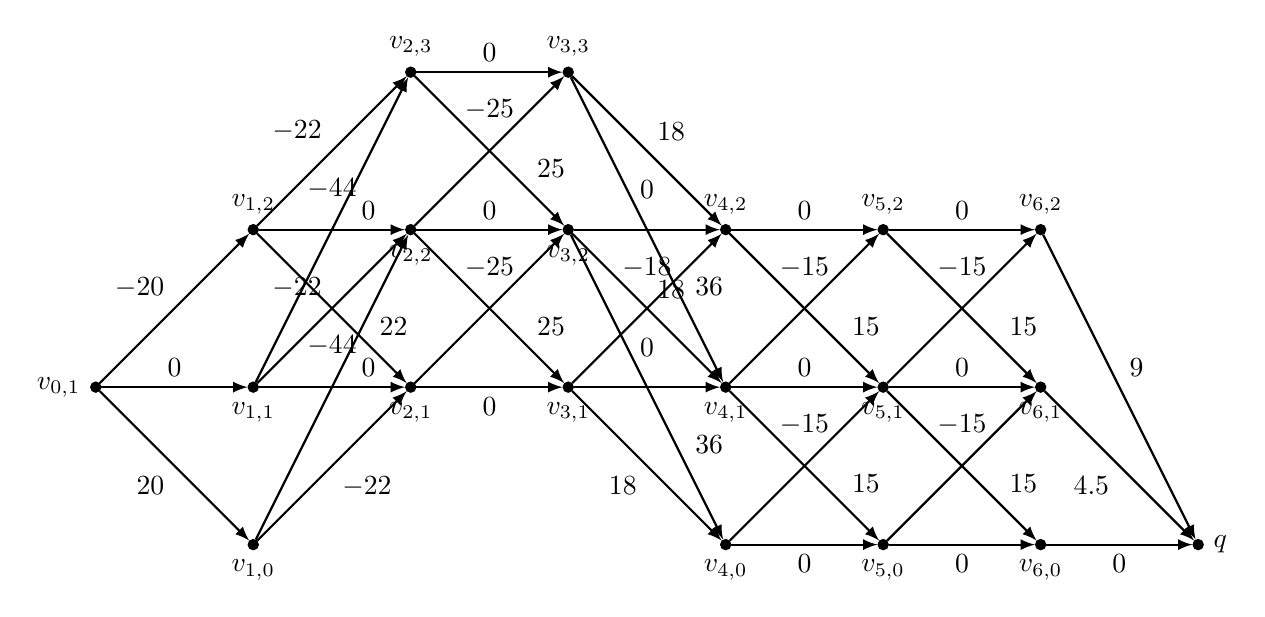
\begin{tikzpicture}

       \tikzset{enclosed/.style={draw, circle, inner sep=0pt, minimum size=.13cm, fill=black}}
%% Vertices
      	\node[enclosed, label={left:  $v_{0,1}$}]   (v1) at  (0,2)  {};
      	\node[enclosed, label={below: $v_{1,0}$}]   (v2) at  (2,0)  {};
    	\node[enclosed, label={below: $v_{1,1}$}]   (v3) at  (2,2)  {};
  	    \node[enclosed, label={above: $v_{1,2}$}]   (v4) at  (2,4)  {};
     	\node[enclosed, label={below: $v_{2,1}$}]   (v5) at  (4,2)  {};
     	\node[enclosed, label={below: $v_{2,2}$}]   (v6) at  (4,4)  {};
     	\node[enclosed, label={above: $v_{2,3}$}]   (v7) at  (4,6)  {};
     	\node[enclosed, label={below: $v_{3,1}$}]   (v8) at  (6,2)  {};
     	\node[enclosed, label={below: $v_{3,2}$}]   (v9) at  (6,4)  {};
     	\node[enclosed, label={above: $v_{3,3}$}]   (v10) at (6,6)  {};
     	\node[enclosed, label={below: $v_{4,0}$}]   (v11) at (8,0)  {};
     	\node[enclosed, label={below: $v_{4,1}$}]   (v12) at (8,2)  {};
      	\node[enclosed, label={above: $v_{4,2}$}]   (v13) at (8,4)  {};
  	    \node[enclosed, label={below: $v_{5,0}$}]   (v14) at (10,0) {};
  	    \node[enclosed, label={below: $v_{5,1}$}]   (v15) at (10,2) {};
     	\node[enclosed, label={above: $v_{5,2}$}]   (v16) at (10,4) {};
     	\node[enclosed, label={below: $v_{6,0}$}]   (v17) at (12,0) {};
     	\node[enclosed, label={below: $v_{6,1}$}]   (v18) at (12,2) {};
     	\node[enclosed, label={above: $v_{6,2}$}]   (v19) at (12,4) {};
     	\node[enclosed, label={right: $q_{\slut}$}] (v20) at (14,0) {};
   
%Edges
		\path[->,>=latex,thick] (v1) edge node[midway, sloped, above, label={below, black: $20$}] {} (v2);
		\path[->,>=latex,thick] (v1) edge node[midway, sloped, below, label={above: $0$ }] {} (v3);
		\path[->,>=latex,thick] (v1) edge node[midway, sloped, below, label={above, black: $-20$ }] {} (v4);
		\path[->,>=latex,thick] (v2) edge node[midway, sloped, above, label={below: $-22$ }] {} (v5);
		\path[->,>=latex,thick] (v2) edge node[midway, above, label={above: $-44$ }] {} (v6);
		\path[->,>=latex,thick] (v3) edge node[near end, sloped, below, label={above: $0$ }] {} (v5);
		\path[->,>=latex,thick] (v3) edge node[midway, sloped, below, label={above: $-22$ }] {} (v6);
		\path[->,>=latex,thick] (v3) edge node[midway, above, label={above: $-44$ }] {} (v7);
		\path[->,>=latex,thick] (v4) edge node[near end, sloped, below, label={above, black: $22$ }] {} (v5);
		\path[->,>=latex,thick] (v4) edge node[near end, sloped, below, label={above, black: $0$ }] {} (v6);		
		\path[->,>=latex,thick] (v4) edge node[midway, sloped, below, label={above: $-22$ }] {} (v7);
		\path[->,>=latex,thick] (v5) edge node[midway, sloped, above, label={below: $0$ }] {} (v8);
		\path[->,>=latex,thick] (v5) edge node[midway, above, label={above: $-25$ }] {} (v9);
		\path[->,>=latex,thick] (v6) edge node[near end, sloped, below, label={above,black: $25$ }] {} (v8);
		\path[->,>=latex,thick] (v6) edge node[midway, sloped, below, label={above: $0$ }] {} (v9);
		\path[->,>=latex,thick] (v6) edge node[midway, above, label={above: $-25$ }] {} (v10);
		\path[->,>=latex,thick] (v7) edge node[near end, sloped, below, label={above: $25$ }] {} (v9);
		\path[->,>=latex,thick] (v7) edge node[midway, sloped, below, label={above: $0$ }] {} (v10);
		\path[->,>=latex,thick] (v8) edge node[midway, sloped, above, label={below,black: $18$ }] {} (v11);
		\path[->,>=latex,thick] (v8) edge node[midway, above, label={above: $0$ }] {} (v12);
		\path[->,>=latex,thick] (v8) edge node[midway, above, label={above: $-18$ }] {} (v13);
		\path[->,>=latex,thick] (v9) edge node[near end, sloped, below, label={above: $36$ }] {} (v11);
		\path[->,>=latex,thick] (v9) edge node[midway, sloped, below, label={above: $18$ }] {} (v12);
		\path[->,>=latex,thick] (v9) edge node[midway, above, label={above: $0$ }] {} (v13);
		\path[->,>=latex,thick] (v10) edge node[near end, sloped, below, label={above: $36$ }] {} (v12);
		\path[->,>=latex,thick] (v10) edge node[midway, sloped, below, label={above: $18$ }] {} (v13);
		\path[->,>=latex,thick] (v11) edge node[midway, sloped, above, label={below,black: $0$ }] {} (v14);
		\path[->,>=latex,thick] (v11) edge node[midway, above, label={above,black: $-15$ }] {} (v15);
		\path[->,>=latex,thick] (v12) edge node[near end, sloped, below, label={above: $15$ }] {} (v14);
		\path[->,>=latex,thick] (v12) edge node[midway, sloped, below, label={above: $0$ }] {} (v15);
		\path[->,>=latex,thick] (v12) edge node[midway, above, label={above: $-15$ }] {} (v16);
		\path[->,>=latex,thick] (v13) edge node[near end, sloped, below, label={above: $15$ }] {} (v15);
		\path[->,>=latex,thick] (v13) edge node[midway, sloped, below, label={above: $0$ }] {} (v16);
		\path[->,>=latex,thick] (v14) edge node[midway, sloped, above, label={below,black: $0$ }] {} (v17);
		\path[->,>=latex,thick] (v14) edge node[midway, above, label={above,black: $-15$ }] {} (v18);
		\path[->,>=latex,thick] (v15) edge node[near end, sloped, below, label={above: $15$ }] {} (v17);
		\path[->,>=latex,thick] (v15) edge node[midway, sloped, below, label={above: $0$ }] {} (v18);
		\path[->,>=latex,thick] (v15) edge node[midway, above, label={above,black: $-15$ }] {} (v19);
		\path[->,>=latex,thick] (v16) edge node[near end, sloped, below, label={above: $15$ }] {} (v18);
		\path[->,>=latex,thick] (v16) edge node[midway, sloped, below, label={above: $0$ }] {} (v19);
		\path[->,>=latex,thick] (v17) edge node[midway, sloped, above, label={below,black: $0$ }] {} (v20);
		\path[->,>=latex,thick] (v18) edge node[midway, sloped, above, label={below,black: $4.5$ }] {} (v20);
		\path[->,>=latex,thick] (v19) edge node[midway, sloped, below, label={above,black: $9$ }] {} (v20);
	\end{tikzpicture}
	\caption{Forsimplet graf for udvidet problem.}
	\label{fig.gaslager_udvidet}
\end{figure}

Vi ønsker igen at maksimere overskuddet og dermed finde den længste vej fra $v_{0,1}$ til $q_{\slut}$. For at løse problemet som et korteste vej-problem ganger vi igen med -1 og får dermed den omvendte graf:

\begin{figure}[H]
\centering
	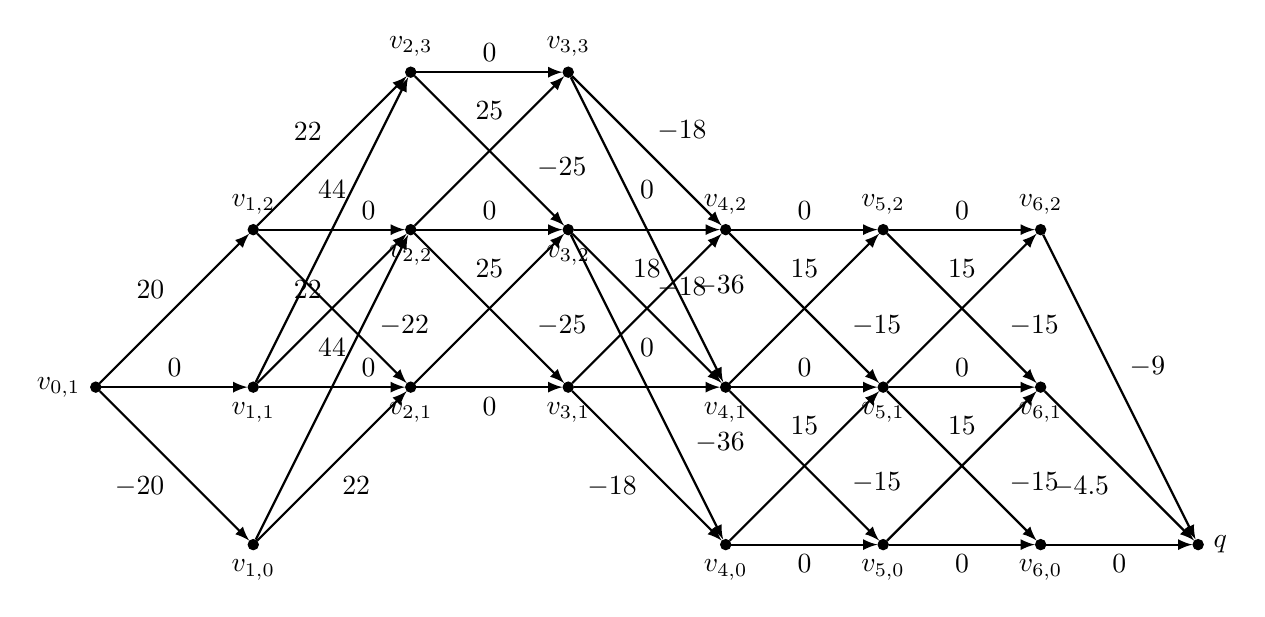
\begin{tikzpicture}

       \tikzset{enclosed/.style={draw, circle, inner sep=0pt, minimum size=.13cm, fill=black}}
%% Vertices
      	\node[enclosed, label={left:  $v_{0,1}$}]   (v1) at  (0,2)  {};
      	\node[enclosed, label={below: $v_{1,0}$}]   (v2) at  (2,0)  {};
    	\node[enclosed, label={below: $v_{1,1}$}]   (v3) at  (2,2)  {};
  	    \node[enclosed, label={above: $v_{1,2}$}]   (v4) at  (2,4)  {};
     	\node[enclosed, label={below: $v_{2,1}$}]   (v5) at  (4,2)  {};
     	\node[enclosed, label={below: $v_{2,2}$}]   (v6) at  (4,4)  {};
     	\node[enclosed, label={above: $v_{2,3}$}]   (v7) at  (4,6)  {};
     	\node[enclosed, label={below: $v_{3,1}$}]   (v8) at  (6,2)  {};
     	\node[enclosed, label={below: $v_{3,2}$}]   (v9) at  (6,4)  {};
     	\node[enclosed, label={above: $v_{3,3}$}]   (v10) at (6,6)  {};
     	\node[enclosed, label={below: $v_{4,0}$}]   (v11) at (8,0)  {};
     	\node[enclosed, label={below: $v_{4,1}$}]   (v12) at (8,2)  {};
      	\node[enclosed, label={above: $v_{4,2}$}]   (v13) at (8,4)  {};
  	    \node[enclosed, label={below: $v_{5,0}$}]   (v14) at (10,0) {};
  	    \node[enclosed, label={below: $v_{5,1}$}]   (v15) at (10,2) {};
     	\node[enclosed, label={above: $v_{5,2}$}]   (v16) at (10,4) {};
     	\node[enclosed, label={below: $v_{6,0}$}]   (v17) at (12,0) {};
     	\node[enclosed, label={below: $v_{6,1}$}]   (v18) at (12,2) {};
     	\node[enclosed, label={above: $v_{6,2}$}]   (v19) at (12,4) {};
     	\node[enclosed, label={right: $q_{\slut}$}] (v20) at (14,0) {};
     	
%Edges
		\path[->,>=latex,thick] (v1) edge node[midway, sloped, above, label={below, black: $-20$}] {} (v2);
		\path[->,>=latex,thick] (v1) edge node[midway, sloped, below, label={above: $0$ }] {} (v3);
		\path[->,>=latex,thick] (v1) edge node[midway, sloped, below, label={above, black: $20$ }] {} (v4);
		\path[->,>=latex,thick] (v2) edge node[midway, sloped, above, label={below: $22$ }] {} (v5);
		\path[->,>=latex,thick] (v2) edge node[midway, above, label={above: $44$ }] {} (v6);
		\path[->,>=latex,thick] (v3) edge node[near end, sloped, below, label={above: $0$ }] {} (v5);
		\path[->,>=latex,thick] (v3) edge node[midway, sloped, below, label={above: $22$ }] {} (v6);
		\path[->,>=latex,thick] (v3) edge node[midway, above, label={above: $44$ }] {} (v7);
		\path[->,>=latex,thick] (v4) edge node[near end, sloped, below, label={above, black: $-22$ }] {} (v5);
		\path[->,>=latex,thick] (v4) edge node[near end, sloped, below, label={above, black: $0$ }] {} (v6);		
		\path[->,>=latex,thick] (v4) edge node[midway, sloped, below, label={above: $22$ }] {} (v7);
		\path[->,>=latex,thick] (v5) edge node[midway, sloped, above, label={below: $0$ }] {} (v8);
		\path[->,>=latex,thick] (v5) edge node[midway, above, label={above: $25$ }] {} (v9);
		\path[->,>=latex,thick] (v6) edge node[near end, sloped, below, label={above,black: $-25$ }] {} (v8);
		\path[->,>=latex,thick] (v6) edge node[midway, sloped, below, label={above: $0$ }] {} (v9);
		\path[->,>=latex,thick] (v6) edge node[midway, above, label={above: $25$ }] {} (v10);
		\path[->,>=latex,thick] (v7) edge node[near end, sloped, below, label={above: $-25$ }] {} (v9);
		\path[->,>=latex,thick] (v7) edge node[midway, sloped, below, label={above: $0$ }] {} (v10);
		\path[->,>=latex,thick] (v8) edge node[midway, sloped, above, label={below,black: $-18$ }] {} (v11);
		\path[->,>=latex,thick] (v8) edge node[midway, above, label={above: $0$ }] {} (v12);
		\path[->,>=latex,thick] (v8) edge node[midway, above, label={above: $18$ }] {} (v13);
		\path[->,>=latex,thick] (v9) edge node[near end, sloped, below, label={above: $-36$ }] {} (v11);
		\path[->,>=latex,thick] (v9) edge node[midway, sloped, below, label={above: $-18$ }] {} (v12);
		\path[->,>=latex,thick] (v9) edge node[midway, above, label={above: $0$ }] {} (v13);
		\path[->,>=latex,thick] (v10) edge node[near end, sloped, below, label={above: $-36$ }] {} (v12);
		\path[->,>=latex,thick] (v10) edge node[midway, sloped, below, label={above: $-18$ }] {} (v13);
		\path[->,>=latex,thick] (v11) edge node[midway, sloped, above, label={below,black: $0$ }] {} (v14);
		\path[->,>=latex,thick] (v11) edge node[midway, above, label={above,black: $15$ }] {} (v15);
		\path[->,>=latex,thick] (v12) edge node[near end, sloped, below, label={above: $-15$ }] {} (v14);
		\path[->,>=latex,thick] (v12) edge node[midway, sloped, below, label={above: $0$ }] {} (v15);
		\path[->,>=latex,thick] (v12) edge node[midway, above, label={above: $15$ }] {} (v16);
		\path[->,>=latex,thick] (v13) edge node[near end, sloped, below, label={above: $-15$ }] {} (v15);
		\path[->,>=latex,thick] (v13) edge node[midway, sloped, below, label={above: $0$ }] {} (v16);
		\path[->,>=latex,thick] (v14) edge node[midway, sloped, above, label={below,black: $0$ }] {} (v17);
		\path[->,>=latex,thick] (v14) edge node[midway, above, label={above,black: $15$ }] {} (v18);
		\path[->,>=latex,thick] (v15) edge node[near end, sloped, below, label={above: $-15$ }] {} (v17);
		\path[->,>=latex,thick] (v15) edge node[midway, sloped, below, label={above: $0$ }] {} (v18);
		\path[->,>=latex,thick] (v15) edge node[midway, above, label={above,black: $15$ }] {} (v19);
		\path[->,>=latex,thick] (v16) edge node[near end, sloped, below, label={above: $-15$ }] {} (v18);
		\path[->,>=latex,thick] (v16) edge node[midway, sloped, below, label={above: $0$ }] {} (v19);
		\path[->,>=latex,thick] (v17) edge node[midway, sloped, above, label={below,black: $0$ }] {} (v20);
		\path[->,>=latex,thick] (v18) edge node[midway, sloped, above, label={below,black: $-4.5$ }] {} (v20);
		\path[->,>=latex,thick] (v19) edge node[midway, sloped, below, label={above,black: $-9$ }] {} (v20);
	\end{tikzpicture}
	\caption{Forsimplet, omvendt graf for udvidet problem.}
	\label{fig.omvendt_udvidet}
\end{figure}

Vi kan nu løse problemet som et korteste vej-problem ved igen at bruge Dijkstras algoritme. Derfor lægger vi nu 40 til alle tal i grafen, så der ikke optræder negative kantvægte. Vi får nu den omvendte graf med udelukkende ikke-negative værdier:


\begin{figure}[H]
\centering
	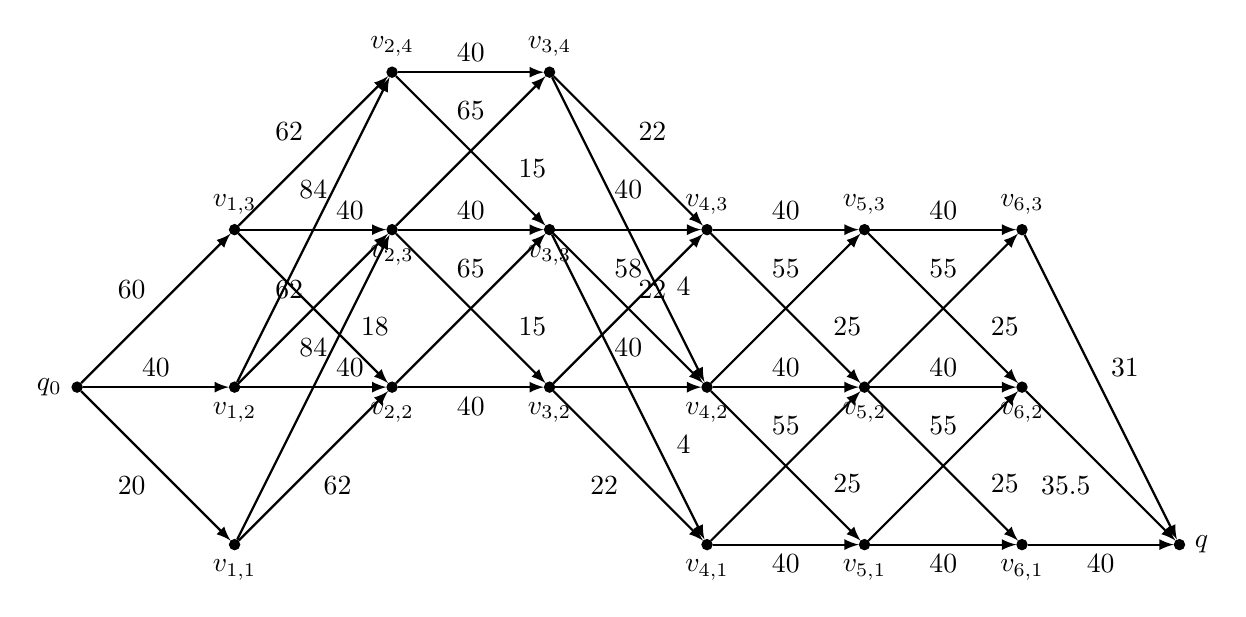
\begin{tikzpicture}

       \tikzset{enclosed/.style={draw, circle, inner sep=0pt, minimum size=.13cm, fill=black}}
%% Vertices
      	\node[enclosed, label={left:  $q_{0}$}]     (v1) at  (0,2)  {};
      	\node[enclosed, label={below: $v_{1,1}$}]   (v2) at  (2,0)  {};
    		\node[enclosed, label={below: $v_{1,2}$}]   (v3) at  (2,2)  {};
  	    \node[enclosed, label={above: $v_{1,3}$}]   (v4) at  (2,4)  {};
     	\node[enclosed, label={below: $v_{2,2}$}]   (v5) at  (4,2)  {};
     	\node[enclosed, label={below: $v_{2,3}$}]   (v6) at  (4,4)  {};
     	\node[enclosed, label={above: $v_{2,4}$}]   (v7) at  (4,6)  {};
     	\node[enclosed, label={below: $v_{3,2}$}]   (v8) at  (6,2)  {};
     	\node[enclosed, label={below: $v_{3,3}$}]   (v9) at  (6,4)  {};
     	\node[enclosed, label={above: $v_{3,4}$}]   (v10) at (6,6)  {};
     	\node[enclosed, label={below: $v_{4,1}$}]   (v11) at (8,0)  {};
     	\node[enclosed, label={below: $v_{4,2}$}]   (v12) at (8,2)  {};
      	\node[enclosed, label={above: $v_{4,3}$}]   (v13) at (8,4)  {};
  	    \node[enclosed, label={below: $v_{5,1}$}]   (v14) at (10,0) {};
  	    \node[enclosed, label={below: $v_{5,2}$}]   (v15) at (10,2) {};
     	\node[enclosed, label={above: $v_{5,3}$}]   (v16) at (10,4) {};
     	\node[enclosed, label={below: $v_{6,1}$}]   (v17) at (12,0) {};
     	\node[enclosed, label={below: $v_{6,2}$}]   (v18) at (12,2) {};
     	\node[enclosed, label={above: $v_{6,3}$}]   (v19) at (12,4) {};
     	\node[enclosed, label={right: $q_{\slut}$}] (v20) at (14,0) {};
     	
%Edges
		\path[->,>=latex,thick] (v1) edge node[midway, sloped, above, label={below, black: $20$}] {} (v2);
		\path[->,>=latex,thick] (v1) edge node[midway, sloped, below, label={above: $40$ }] {} (v3);
		\path[->,>=latex,thick] (v1) edge node[midway, sloped, below, label={above, black: $60$ }] {} (v4);
		\path[->,>=latex,thick] (v2) edge node[midway, sloped, above, label={below: $62$ }] {} (v5);
		\path[->,>=latex,thick] (v2) edge node[midway, above, label={above: $84$ }] {} (v6);
		\path[->,>=latex,thick] (v3) edge node[near end, sloped, below, label={above: $40$ }] {} (v5);
		\path[->,>=latex,thick] (v3) edge node[midway, sloped, below, label={above: $62$ }] {} (v6);
		\path[->,>=latex,thick] (v3) edge node[midway, above, label={above: $84$ }] {} (v7);
		\path[->,>=latex,thick] (v4) edge node[near end, sloped, below, label={above, black: $18$ }] {} (v5);
		\path[->,>=latex,thick] (v4) edge node[near end, sloped, below, label={above, black: $40$ }] {} (v6);		
		\path[->,>=latex,thick] (v4) edge node[midway, sloped, below, label={above: $62$ }] {} (v7);
		\path[->,>=latex,thick] (v5) edge node[midway, sloped, above, label={below: $40$ }] {} (v8);
		\path[->,>=latex,thick] (v5) edge node[midway, above, label={above: $65$ }] {} (v9);
		\path[->,>=latex,thick] (v6) edge node[near end, sloped, below, label={above,black: $15$ }] {} (v8);
		\path[->,>=latex,thick] (v6) edge node[midway, sloped, below, label={above: $40$ }] {} (v9);
		\path[->,>=latex,thick] (v6) edge node[midway, above, label={above: $65$ }] {} (v10);
		\path[->,>=latex,thick] (v7) edge node[near end, sloped, below, label={above: $15$ }] {} (v9);
		\path[->,>=latex,thick] (v7) edge node[midway, sloped, below, label={above: $40$ }] {} (v10);
		\path[->,>=latex,thick] (v8) edge node[midway, sloped, above, label={below,black: $22$ }] {} (v11);
		\path[->,>=latex,thick] (v8) edge node[midway, above, label={above: $40$ }] {} (v12);
		\path[->,>=latex,thick] (v8) edge node[midway, above, label={above: $58$ }] {} (v13);
		\path[->,>=latex,thick] (v9) edge node[near end, sloped, below, label={above: $4$ }] {} (v11);
		\path[->,>=latex,thick] (v9) edge node[midway, sloped, below, label={above: $22$ }] {} (v12);
		\path[->,>=latex,thick] (v9) edge node[midway, above, label={above: $40$ }] {} (v13);
		\path[->,>=latex,thick] (v10) edge node[near end, sloped, below, label={above: $4$ }] {} (v12);
		\path[->,>=latex,thick] (v10) edge node[midway, sloped, below, label={above: $22$ }] {} (v13);
		\path[->,>=latex,thick] (v11) edge node[midway, sloped, above, label={below,black: $40$ }] {} (v14);
		\path[->,>=latex,thick] (v11) edge node[midway, above, label={above,black: $55$ }] {} (v15);
		\path[->,>=latex,thick] (v12) edge node[near end, sloped, below, label={above: $25$ }] {} (v14);
		\path[->,>=latex,thick] (v12) edge node[midway, sloped, below, label={above: $40$ }] {} (v15);
		\path[->,>=latex,thick] (v12) edge node[midway, above, label={above: $55$ }] {} (v16);
		\path[->,>=latex,thick] (v13) edge node[near end, sloped, below, label={above: $25$ }] {} (v15);
		\path[->,>=latex,thick] (v13) edge node[midway, sloped, below, label={above: $40$ }] {} (v16);
		\path[->,>=latex,thick] (v14) edge node[midway, sloped, above, label={below,black: $40$ }] {} (v17);
		\path[->,>=latex,thick] (v14) edge node[midway, above, label={above,black: $55$ }] {} (v18);
		\path[->,>=latex,thick] (v15) edge node[near end, sloped, below, label={above: $25$ }] {} (v17);
		\path[->,>=latex,thick] (v15) edge node[midway, sloped, below, label={above: $40$ }] {} (v18);
		\path[->,>=latex,thick] (v15) edge node[midway, above, label={above,black: $55$ }] {} (v19);
		\path[->,>=latex,thick] (v16) edge node[near end, sloped, below, label={above: $25$ }] {} (v18);
		\path[->,>=latex,thick] (v16) edge node[midway, sloped, below, label={above: $40$ }] {} (v19);
		\path[->,>=latex,thick] (v17) edge node[midway, sloped, above, label={below,black: $40$ }] {} (v20);
		\path[->,>=latex,thick] (v18) edge node[midway, sloped, above, label={below,black: $35.5$ }] {} (v20);
		\path[->,>=latex,thick] (v19) edge node[midway, sloped, below, label={above,black: $31$ }] {} (v20);
	\end{tikzpicture}
	\caption{Omvendt, positiv, udvidet graf.}
	\label{fig.omvendt_udvidet}
\end{figure}

Vi kan på samme måde som ved basisproblemet opstille en tabel over de mulige veje gennem grafen fra $v_{0,1}$ til $q_{\slut}$:

\begin{table}[H]
\centering
\begin{tabular}{|c|c|c|c|c|c|c|c|c|c|c|c|c|c|} 
\hline
$n$ & $R_{n} \bigcup$ & $q_{0}$ & $v_{1,1}$ & $v_{1,2}$ & $v_{1,3}$ & $v_{2,2}$ & $v_{2,3}$ & $v_{2,4}$ & $\ldots$ & $v_{6,1}$ & $v_{6,2}$ & $v_{6,3}$ & $q_{slut}$ \\
\hline
0 & $\emptyset$ & 0 & $\infty$ & $\infty$ & $\infty$ & $\infty$ & $\infty$ & $\infty$ & $\ldots$ & $\infty$ & $\infty$ & $\infty$ & $\infty$ \\ 
1 & $q_{0}$ & & 20 & 40 & 60 & $\infty$ & $\infty$ & $\infty$ & $\ldots$ & $\infty$ & $\infty$ & $\infty$ & $\infty$\\ 
2 & $v_{1,1}$ & & & 40 & 60 & 82 & 104 & $\infty$ & $\ldots$ & $\infty$ & $\infty$ & $\infty$ & $\infty$\\ 
3 & $v_{1,2}$ & & & & 60 & 80 & 102 & 124 & $\ldots$ & $\infty$ & $\infty$ & $\infty$ & $\infty$\\
4 & $v_{1,3}$ & & & & & 78 & 100 & 122 & $\ldots$ & $\infty$ & $\infty$ & $\infty$ & $\infty$\\ 
5 & $v_{2,2}$ & & & & & & 100 & 122 & $\ldots$ & $\infty$ & $\infty$ & $\infty$ & $\infty$\\ 
6 & $v_{2,3}$ & & & & & & & 122 & $\ldots$ & $\infty$ & $\infty$ & $\infty$ & $\infty$\\  
$\vdots$ & $\vdots$ & $\vdots$ & $\vdots$ & $\vdots$ & $\vdots$ & $\vdots$ & $\vdots$ & $\vdots$ &  & $\vdots$ & $\vdots$ & $\vdots$ & $\vdots$\\ 
14 & $v_{5,1}$ &  &  &  &  &  &  &  & $\ldots$ & 217 & 232 & $\infty$ & $\infty$\\ 
15 & $v_{5,2}$ &  &  &  &  &  &  &  & $\ldots$ & 217 & 232 & 247 & $\infty$\\ 
16 & $v_{5,3}$ &  &  &  &  &  &  &  & $\ldots$ & 217 & 232 & 247 & $\infty$\\ 
17 & $v_{6,1}$ &  &  &  &  &  &  &  & $\ldots$ &  & 232 & 247 & 257\\ 
18 & $v_{6,2}$ &  &  &  &  &  &  &  & $\ldots$ &  &  & 247 & 257\\ 
18 & $v_{6,3}$ &  &  &  &  &  &  &  & $\ldots$ &  &  &  & 257\\ 
\hline
\end{tabular}
\caption{Tabel over veje gennem forsimplet, udvidet graf.}
\label{table:forsimplet_udvidet_graf}
\end{table} 


Beregningerne foregår på samme vis som i \autoref{table:forsimplet_graf}. Vi får dermed, at vi har to forskellige veje fra $v_{0,1}$ til $q_{\slut}$, som begge har distancen 257. I den oprindelige graf i \autoref{fig.gaslager_udvidet} havde kanterne andre vægte, som vi nu kan indsætte igen efter brugen af Dijkstras algoritme. Vejen går igennem de samme knuder, og ønsker vi at finde distancen fra $v_{0,1}$ til $q_{\slut}$, skal vi blot tage vores resultat og trække de 40, som vi adderede hver kant med, fra 7 gange, altså en gang for hver kant i vejen fra $v_{0,1}$ til $q_{\slut}$. Derefter ganger vi med -1.
\begin{equation}
(257-40 \cdot 7)(-1) = 23.
\end{equation}
Vejene illustreres på \autoref{fig:gaslager_udvidet}:

\begin{figure}[H]
\centering
	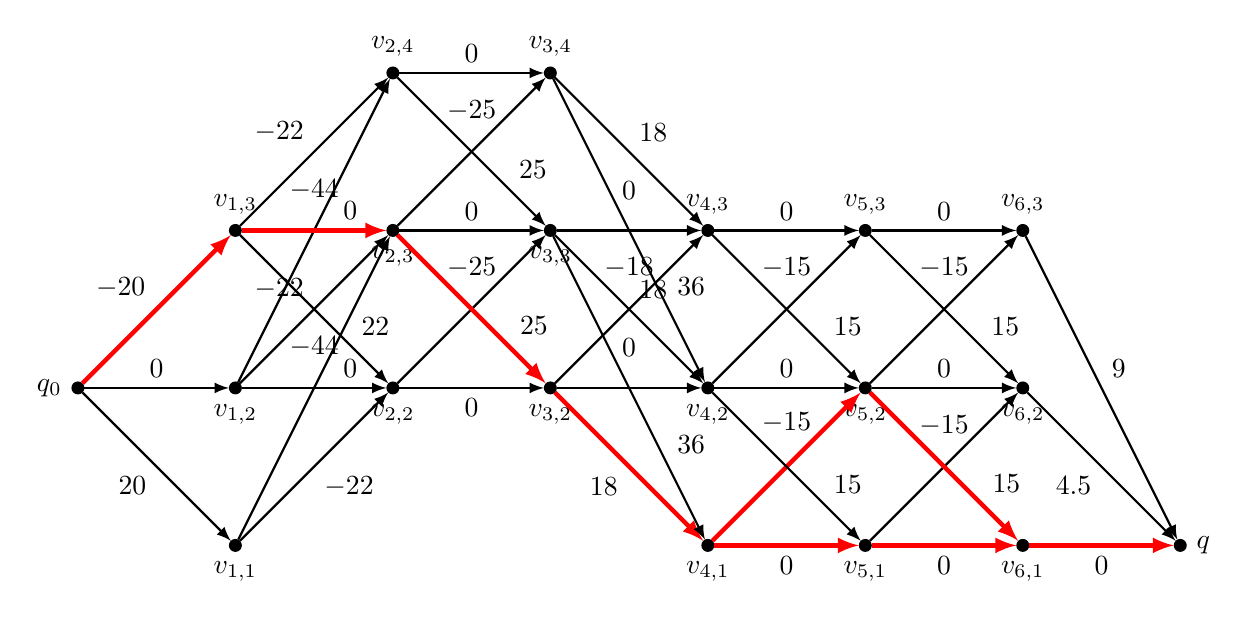
\begin{tikzpicture}

       \tikzset{enclosed/.style={draw, circle, inner sep=0pt, minimum size=.15cm, fill=black}}
%% Vertices
      	\node[enclosed, label={left:  $q_{0}$}]     (v1) at  (0,2)  {};
      	\node[enclosed, label={below: $v_{1,1}$}]   (v2) at  (2,0)  {};
    		\node[enclosed, label={below: $v_{1,2}$}]   (v3) at  (2,2)  {};
  	    \node[enclosed, label={above: $v_{1,3}$}]   (v4) at  (2,4)  {};
     	\node[enclosed, label={below: $v_{2,2}$}]   (v5) at  (4,2)  {};
     	\node[enclosed, label={below: $v_{2,3}$}]   (v6) at  (4,4)  {};
     	\node[enclosed, label={above: $v_{2,4}$}]   (v7) at  (4,6)  {};
     	\node[enclosed, label={below: $v_{3,2}$}]   (v8) at  (6,2)  {};
     	\node[enclosed, label={below: $v_{3,3}$}]   (v9) at  (6,4)  {};
     	\node[enclosed, label={above: $v_{3,4}$}]   (v10) at (6,6)  {};
     	\node[enclosed, label={below: $v_{4,1}$}]   (v11) at (8,0)  {};
     	\node[enclosed, label={below: $v_{4,2}$}]   (v12) at (8,2)  {};
      	\node[enclosed, label={above: $v_{4,3}$}]   (v13) at (8,4)  {};
  	    \node[enclosed, label={below: $v_{5,1}$}]   (v14) at (10,0) {};
  	    \node[enclosed, label={below: $v_{5,2}$}]   (v15) at (10,2) {};
     	\node[enclosed, label={above: $v_{5,3}$}]   (v16) at (10,4) {};
     	\node[enclosed, label={below: $v_{6,1}$}]   (v17) at (12,0) {};
     	\node[enclosed, label={below: $v_{6,2}$}]   (v18) at (12,2) {};
     	\node[enclosed, label={above: $v_{6,3}$}]   (v19) at (12,4) {};
     	\node[enclosed, label={right: $q_{\slut}$}] (v20) at (14,0) {};
     	
%Edges
		\path[->,>=latex,thick] (v1) edge node[midway, sloped, above, label={below, black: $20$}] {} (v2);
		\path[->,>=latex,thick] (v1) edge node[midway, sloped, below, label={above: $0$ }] {} (v3);
		\path[red,->,>=latex,ultra thick] (v1) edge node[midway, sloped, below, label={above, black: $-20$ }] {} (v4);
		\path[->,>=latex,thick] (v2) edge node[midway, sloped, above, label={below: $-22$ }] {} (v5);
		\path[->,>=latex,thick] (v2) edge node[midway, above, label={above: $-44$ }] {} (v6);
		\path[->,>=latex,thick] (v3) edge node[near end, sloped, below, label={above: $0$ }] {} (v5);
		\path[->,>=latex,thick] (v3) edge node[midway, sloped, below, label={above: $-22$ }] {} (v6);
		\path[->,>=latex,thick] (v3) edge node[midway, above, label={above: $-44$ }] {} (v7);
		\path[->,>=latex,thick] (v4) edge node[near end, sloped, below, label={above, black: $22$ }] {} (v5);
		\path[red,->,>=latex,ultra thick] (v4) edge node[near end, sloped, below, label={above, black: $0$ }] {} (v6);		
		\path[->,>=latex,thick] (v4) edge node[midway, sloped, below, label={above: $-22$ }] {} (v7);
		\path[->,>=latex,thick] (v5) edge node[midway, sloped, above, label={below: $0$ }] {} (v8);
		\path[->,>=latex,thick] (v5) edge node[midway, above, label={above: $-25$ }] {} (v9);
		\path[red,->,>=latex,ultra thick] (v6) edge node[near end, sloped, below, label={above,black: $25$ }] {} (v8);
		\path[->,>=latex,thick] (v6) edge node[midway, sloped, below, label={above: $0$ }] {} (v9);
		\path[->,>=latex,thick] (v6) edge node[midway, above, label={above: $-25$ }] {} (v10);
		\path[->,>=latex,thick] (v7) edge node[near end, sloped, below, label={above: $25$ }] {} (v9);
		\path[->,>=latex,thick] (v7) edge node[midway, sloped, below, label={above: $0$ }] {} (v10);
		\path[red,->,>=latex,ultra thick] (v8) edge node[midway, sloped, above, label={below,black: $18$ }] {} (v11);
		\path[->,>=latex,thick] (v8) edge node[midway, above, label={above: $0$ }] {} (v12);
		\path[->,>=latex,thick] (v8) edge node[midway, above, label={above: $-18$ }] {} (v13);
		\path[->,>=latex,thick] (v9) edge node[near end, sloped, below, label={above: $36$ }] {} (v11);
		\path[->,>=latex,thick] (v9) edge node[midway, sloped, below, label={above: $18$ }] {} (v12);
		\path[->,>=latex,thick] (v9) edge node[midway, above, label={above: $0$ }] {} (v13);
		\path[->,>=latex,thick] (v10) edge node[near end, sloped, below, label={above: $36$ }] {} (v12);
		\path[->,>=latex,thick] (v10) edge node[midway, sloped, below, label={above: $18$ }] {} (v13);
		\path[red,->,>=latex,ultra thick] (v11) edge node[midway, sloped, above, label={below,black: $0$ }] {} (v14);
		\path[red,->,>=latex,ultra thick] (v11) edge node[midway, above, label={above,black: $-15$ }] {} (v15);
		\path[->,>=latex,thick] (v12) edge node[near end, sloped, below, label={above: $15$ }] {} (v14);
		\path[->,>=latex,thick] (v12) edge node[midway, sloped, below, label={above: $0$ }] {} (v15);
		\path[->,>=latex,thick] (v12) edge node[midway, above, label={above: $-15$ }] {} (v16);
		\path[->,>=latex,thick] (v13) edge node[near end, sloped, below, label={above: $15$ }] {} (v15);
		\path[->,>=latex,thick] (v13) edge node[midway, sloped, below, label={above: $0$ }] {} (v16);
		\path[red,->,>=latex,ultra thick] (v14) edge node[midway, sloped, above, label={below,black: $0$ }] {} (v17);
		\path[->,>=latex,thick] (v14) edge node[midway, above, label={above,black: $-15$ }] {} (v18);
		\path[red,->,>=latex,ultra thick] (v15) edge node[near end, sloped, below, label={above,black: $15$ }] {} (v17);
		\path[->,>=latex,thick] (v15) edge node[midway, sloped, below, label={above: $0$ }] {} (v18);
		\path[->,>=latex,thick] (v15) edge node[midway, above, label={above,black: $-15$ }] {} (v19);
		\path[->,>=latex,thick] (v16) edge node[near end, sloped, below, label={above: $15$ }] {} (v18);
		\path[->,>=latex,thick] (v16) edge node[midway, sloped, below, label={above: $0$ }] {} (v19);
		\path[red,->,>=latex,ultra thick] (v17) edge node[midway, sloped, above, label={below,black: $0$ }] {} (v20);
		\path[->,>=latex,thick] (v18) edge node[midway, sloped, above, label={below,black: $4.5$ }] {} (v20);
		\path[->,>=latex,thick] (v19) edge node[midway, sloped, below, label={above,black: $9$ }] {} (v20);
	\end{tikzpicture}
	\caption{Graf for den længste vej igennem grafen.}
	\label{fig.gaslager_udvidet}
\end{figure}



\section{Det udvidede problem som algoritme}
Vi arbejder med den samme algoritme, som vi gjorde i basisproblemet, da denne var tilpasset eventuelle udvidelser og genereliseringer. Den eneste forskel er vores data:

\lstinputlisting[
  firstline=36,
  lastline=57,
  label={code:data_udvidet},
  caption={Definering af data for det udvidede problem.}
]{code/dijkstras.py} 

Det ses, at de tidligere statiske værdier, $q_{max}$, $q_{min}$, $i_{max}$ og $u_{max}$ nu ændrer sig alt efter, hvilken måned vi befinder os i. Dette ændrer også resultatet, og sættes dataen ind i algoritmen fås nu:

\begin{lstlisting} [label=lst:udvidet_output,caption=Output for det udvidede problem.]

The highest profit is 188.29 Euro
The path is $['q0.5', 'q1.8', 'q2.4', 'q3.2', 'q4.4', 'q5.5', 'q6.6', 'q7.7', 'q8.8', 'q9.8', 'q10.10', 'q11.9', 'q12.5', 'q_slut']$,

\end{lstlisting}

\subsection{Resultatbehandling af det udvidede problem} \label{kap:resultat_udvidet}

Vi kigger i dette afsnit på de resultater, vores algoritme har fundet i det udvidede problem. Den længste vej er fundet ved brug af vores korteste-vej algoritme med fremgangsmåden, som er gennemgået i \autoref{kap:grafen_for_udvidet}. På \ref{fig:gaslager_graf_udvidet} kan man se den længste vej igennem grafen for det udvidede problem.
\begin{figure}[H]
\centering
	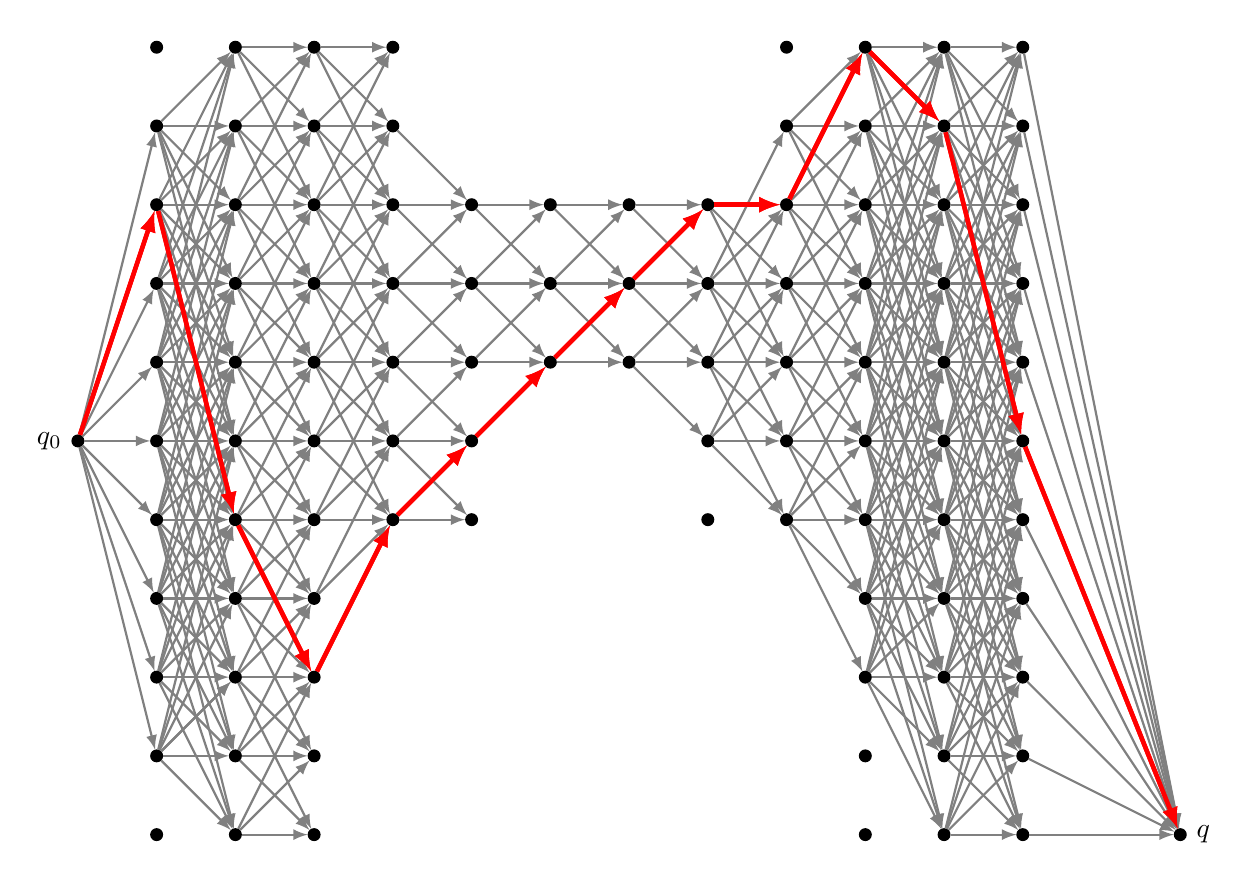
\begin{tikzpicture}

       \tikzset{enclosed/.style={draw, circle, inner sep=0pt, minimum size=.15cm, fill=black}}
%% Vertices
      	\node[enclosed, label={left: $q_{0}$}] (vstart) at (-1,5) {};
      	\node[enclosed, label={below: }] (v00) at (0,0) {};
    		\node[enclosed, label={below: }] (v01) at (0,1) {};
  	    \node[enclosed, label={above: }] (v02) at (0,2) {};
     	\node[enclosed, label={below: }] (v03) at (0,3) {};
     	\node[enclosed, label={below:  }] (v04) at (0,4) {};
     	\node[enclosed, label={above: }] (v05) at (0,5) {};
     	\node[enclosed, label={below: }] (v06) at (0,6) {};
     	\node[enclosed, label={below: }] (v07) at (0,7) {};
     	\node[enclosed, label={above: }] (v08) at (0,8) {};
     	\node[enclosed, label={below:  }] (v09) at (0,9) {};
     	\node[enclosed, label={below: }] (v010) at (0,10) {};
      	\node[enclosed, label={above: }] (v10) at (1,0) {};
  	    \node[enclosed, label={below: }] (v11) at (1,1) {};
  	    \node[enclosed, label={below: }] (v12) at (1,2) {};
     	\node[enclosed, label={above:  }] (v13) at (1,3) {};
     	\node[enclosed, label={below: }] (v14) at (1,4) {};
     	 \node[enclosed, label={below:}] (v15) at (1,5) {};
     	\node[enclosed, label={above: }] (v16) at (1,6) {};
     	\node[enclosed, label={below: }] (v17) at (1,7) {};
     	\node[enclosed, label={above: }] (v18) at (1,8) {};
     	\node[enclosed, label={below:  }] (v19) at (1,9) {};
     	\node[enclosed, label={below: }] (v110) at (1,10) {};
     	\node[enclosed, label={below: }] (v20) at (2,0) {};
    		\node[enclosed, label={below: }] (v21) at (2,1) {};
  	    \node[enclosed, label={above: }] (v22) at (2,2) {};
     	\node[enclosed, label={below: }] (v23) at (2,3) {};
     	\node[enclosed, label={below:  }] (v24) at (2,4) {};
     	\node[enclosed, label={above: }] (v25) at (2,5) {};
     	\node[enclosed, label={below: }] (v26) at (2,6) {};
     	\node[enclosed, label={below: }] (v27) at (2,7) {};
     	\node[enclosed, label={above: }] (v28) at (2,8) {};
     	\node[enclosed, label={below:  }] (v29) at (2,9) {};
     	\node[enclosed, label={below: }] (v210) at (2,10) {};
     	\node[enclosed, label={below: }] (v34) at (3,4) {};
     	 \node[enclosed, label={below:}] (v35) at (3,5) {};
     	\node[enclosed, label={above: }] (v36) at (3,6) {};
     	\node[enclosed, label={below: }] (v37) at (3,7) {};
     	\node[enclosed, label={above: }] (v38) at (3,8) {};
     	\node[enclosed, label={below:  }] (v39) at (3,9) {};
     	\node[enclosed, label={below: }] (v310) at (3,10) {};
     	\node[enclosed, label={below:  }] (v44) at (4,4) {};
     	\node[enclosed, label={above: }] (v45) at (4,5) {};
     	\node[enclosed, label={below: }] (v46) at (4,6) {};
     	\node[enclosed, label={below: }] (v47) at (4,7) {};
     	\node[enclosed, label={above: }] (v48) at (4,8) {};
     	\node[enclosed, label={above: }] (v56) at (5,6) {};
     	\node[enclosed, label={below: }] (v57) at (5,7) {};
     	\node[enclosed, label={above: }] (v58) at (5,8) {};
     	\node[enclosed, label={below: }] (v66) at (6,6) {};
     	\node[enclosed, label={below: }] (v67) at (6,7) {};
     	\node[enclosed, label={above: }] (v68) at (6,8) {};
     	\node[enclosed, label={below: }] (v74) at (7,4) {};
     	 \node[enclosed, label={below:}] (v75) at (7,5) {};
     	\node[enclosed, label={above: }] (v76) at (7,6) {};
     	\node[enclosed, label={below: }] (v77) at (7,7) {};
     	\node[enclosed, label={above: }] (v78) at (7,8) {};
     	\node[enclosed, label={below: }] (v84) at (8,4) {};
     	 \node[enclosed, label={below:}] (v85) at (8,5) {};
     	\node[enclosed, label={above: }] (v86) at (8,6) {};
     	\node[enclosed, label={below: }] (v87) at (8,7) {};
     	\node[enclosed, label={above: }] (v88) at (8,8) {};
     	\node[enclosed, label={below:  }] (v89) at (8,9) {};
     	\node[enclosed, label={below: }] (v810) at (8,10) {};
     	\node[enclosed, label={below: }] (v90) at (9,0) {};
    		\node[enclosed, label={below: }] (v91) at (9,1) {};
  	    \node[enclosed, label={above: }] (v92) at (9,2) {};
     	\node[enclosed, label={below: }] (v93) at (9,3) {};
     	\node[enclosed, label={below:  }] (v94) at (9,4) {};
     	\node[enclosed, label={above: }] (v95) at (9,5) {};
     	\node[enclosed, label={below: }] (v96) at (9,6) {};
     	\node[enclosed, label={below: }] (v97) at (9,7) {};
     	\node[enclosed, label={above: }] (v98) at (9,8) {};
     	\node[enclosed, label={below:  }] (v99) at (9,9) {};
     	\node[enclosed, label={below: }] (v910) at (9,10) {};
      	\node[enclosed, label={above: }] (v100) at (10,0) {};
  	    \node[enclosed, label={below: }] (v101) at (10,1) {};
  	    \node[enclosed, label={below: }] (v102) at (10,2) {};
     	\node[enclosed, label={above:  }] (v103) at (10,3) {};
     	\node[enclosed, label={below: }] (v104) at (10,4) {};
     	 \node[enclosed, label={below:}] (v105) at (10,5) {};
     	\node[enclosed, label={above: }] (v106) at (10,6) {};
     	\node[enclosed, label={below: }] (v107) at (10,7) {};
     	\node[enclosed, label={above: }] (v108) at (10,8) {};
     	\node[enclosed, label={below:  }] (v109) at (10,9) {};
     	\node[enclosed, label={below: }] (v1010) at (10,10) {};
     	\node[enclosed, label={above: }] (v1100) at (11,0) {};
  	    \node[enclosed, label={below: }] (v111) at (11,1) {};
  	    \node[enclosed, label={below: }] (v112) at (11,2) {};
     	\node[enclosed, label={above:  }] (v113) at (11,3) {};
     	\node[enclosed, label={below: }] (v114) at (11,4) {};
     	 \node[enclosed, label={below:}] (v115) at (11,5) {};
     	\node[enclosed, label={above: }] (v116) at (11,6) {};
     	\node[enclosed, label={below: }] (v117) at (11,7) {};
     	\node[enclosed, label={above: }] (v118) at (11,8) {};
     	\node[enclosed, label={below:  }] (v119) at (11,9) {};
     	\node[enclosed, label={below: }] (v1110) at (11,10) {};
     	\node[enclosed, label={right: $q_{\slut}$ }] (v120) at (13,0) {};
     	
%Edges
		\path[gray,->,>=latex,thick] (vstart) edge node[midway, sloped, above] {} (v01);
		\path[gray,->,>=latex,thick] (vstart) edge node[midway, sloped, below] {} (v02);
		\path[gray,->,>=latex,thick] (vstart) edge node[midway, sloped, below] {} (v03);
		\path[gray,->,>=latex,thick] (vstart) edge node[midway, sloped, above] {} (v04);
		\path[gray,->,>=latex,thick] (vstart) edge node[midway, above] {} (v05);
		\path[gray,->,>=latex,thick] (vstart) edge node[near end, sloped, below] {} (v06);
		\path[gray,->,>=latex,thick] (vstart) edge node[midway, sloped, below] {} (v07);
		\path[red,->,>=latex,ultra thick] (vstart) edge node[midway, above] {} (v08);
		\path[gray,->,>=latex,thick] (vstart) edge node[near end, sloped, below] {} (v09);
		\path[gray,->,>=latex,thick] (v01) edge node[midway, sloped, below] {} (v10);
		\path[gray,->,>=latex,thick] (v01) edge node[midway, sloped, above] {} (v11);
		\path[gray,->,>=latex,thick] (v01) edge node[midway, above] {} (v12);
		\path[gray,->,>=latex,thick] (v01) edge node[near end, sloped, below] {} (v12);
		\path[gray,->,>=latex,thick] (v01) edge node[midway, sloped, below] {} (v13);
		\path[gray,->,>=latex,thick] (v01) edge node[midway, above] {} (v14);
		\path[gray,->,>=latex,thick] (v01) edge node[near end, sloped, below] {} (v15);
		\path[gray,->,>=latex,thick] (v02) edge node[midway, sloped, below] {} (v10);
		\path[gray,->,>=latex,thick] (v02) edge node[midway, sloped, above] {} (v11);
		\path[gray,->,>=latex,thick] (v02) edge node[midway, above] {} (v12);
		\path[gray,->,>=latex,thick] (v02) edge node[near end, sloped, below] {} (v13);
		\path[gray,->,>=latex,thick] (v02) edge node[midway, sloped, below] {} (v14);
		\path[gray,->,>=latex,thick] (v02) edge node[midway, above] {} (v15);
		\path[gray,->,>=latex,thick] (v02) edge node[near end, sloped, below] {} (v16);
		\path[gray,->,>=latex,thick] (v03) edge node[midway, sloped, below] {} (v10);
		\path[gray,->,>=latex,thick] (v03) edge node[midway, sloped, above] {} (v11);
		\path[gray,->,>=latex,thick] (v03) edge node[midway, above] {} (v12);
		\path[gray,->,>=latex,thick] (v03) edge node[near end, sloped, below] {} (v13);
		\path[gray,->,>=latex,thick] (v03) edge node[midway, sloped, below] {} (v14);
		\path[gray,->,>=latex,thick] (v03) edge node[midway, above] {} (v15);
		\path[gray,->,>=latex,thick] (v03) edge node[near end, sloped, below] {} (v16);
		\path[gray,->,>=latex,thick] (v03) edge node[midway, sloped, below] {} (v17);
		\path[gray,->,>=latex,thick] (v04) edge node[midway, sloped, below] {} (v10);
		\path[gray,->,>=latex,thick] (v04) edge node[midway, sloped, above] {} (v11);
		\path[gray,->,>=latex,thick] (v04) edge node[midway, above] {} (v12);
		\path[gray,->,>=latex,thick] (v04) edge node[near end, sloped, below] {} (v13);
		\path[gray,->,>=latex,thick] (v04) edge node[midway, sloped, below] {} (v14);
		\path[gray,->,>=latex,thick] (v04) edge node[midway, above] {} (v15);
		\path[gray,->,>=latex,thick] (v04) edge node[near end, sloped, below] {} (v16);
		\path[gray,->,>=latex,thick] (v04) edge node[midway, sloped, below] {} (v17);
		\path[gray,->,>=latex,thick] (v04) edge node[midway, sloped, above] {} (v18);
		\path[gray,->,>=latex,thick] (v05) edge node[midway, sloped, above] {} (v11);
		\path[gray,->,>=latex,thick] (v05) edge node[midway, above] {} (v12);
		\path[gray,->,>=latex,thick] (v05) edge node[near end, sloped, below] {} (v13);
		\path[gray,->,>=latex,thick] (v05) edge node[midway, sloped, below] {} (v14);
		\path[gray,->,>=latex,thick] (v05) edge node[midway, above] {} (v15);
		\path[gray,->,>=latex,thick] (v05) edge node[near end, sloped, below] {} (v16);
		\path[gray,->,>=latex,thick] (v05) edge node[midway, sloped, below] {} (v17);
		\path[gray,->,>=latex,thick] (v05) edge node[midway, sloped, above] {} (v18);
		\path[gray,->,>=latex,thick] (v05) edge node[midway, sloped, above] {} (v19);
		\path[gray,->,>=latex,thick] (v06) edge node[midway, above] {} (v12);
		\path[gray,->,>=latex,thick] (v06) edge node[near end, sloped, below] {} (v13);
		\path[gray,->,>=latex,thick] (v06) edge node[midway, sloped, below] {} (v14);
		\path[gray,->,>=latex,thick] (v06) edge node[midway, above] {} (v15);
		\path[gray,->,>=latex,thick] (v06) edge node[near end, sloped, below] {} (v16);
		\path[gray,->,>=latex,thick] (v06) edge node[midway, sloped, below] {} (v17);
		\path[gray,->,>=latex,thick] (v06) edge node[midway, sloped, above] {} (v18);
		\path[gray,->,>=latex,thick] (v06) edge node[midway, sloped, above] {} (v19);
		\path[gray,->,>=latex,thick] (v06) edge node[midway, sloped, above] {} (v110);
		\path[gray,->,>=latex,thick] (v07) edge node[near end, sloped, below] {} (v13);
		\path[gray,->,>=latex,thick] (v07) edge node[midway, sloped, below] {} (v14);
		\path[gray,->,>=latex,thick] (v07) edge node[midway, above] {} (v15);
		\path[gray,->,>=latex,thick] (v07) edge node[near end, sloped, below] {} (v16);
		\path[gray,->,>=latex,thick] (v07) edge node[midway, sloped, below] {} (v17);
		\path[gray,->,>=latex,thick] (v07) edge node[midway, sloped, above] {} (v18);
		\path[gray,->,>=latex,thick] (v07) edge node[midway, sloped, above] {} (v19);
		\path[gray,->,>=latex,thick] (v07) edge node[midway, sloped, above] {} (v110);
		\path[red,->,>=latex,ultra thick] (v08) edge node[midway, sloped, below] {} (v14);
		\path[gray,->,>=latex,thick] (v08) edge node[midway, above] {} (v15);
		\path[gray,->,>=latex,thick] (v08) edge node[near end, sloped, below] {} (v16);
		\path[gray,->,>=latex,thick] (v08) edge node[midway, sloped, below] {} (v17);
		\path[gray,->,>=latex,thick] (v08) edge node[midway, sloped, above] {} (v18);
		\path[gray,->,>=latex,thick] (v08) edge node[midway, sloped, above] {} (v19);
		\path[gray,->,>=latex,thick] (v08) edge node[midway, sloped, above] {} (v110);
		\path[gray,->,>=latex,thick] (v09) edge node[midway, above] {} (v15);
		\path[gray,->,>=latex,thick] (v09) edge node[near end, sloped, below] {} (v16);
		\path[gray,->,>=latex,thick] (v09) edge node[midway, sloped, below] {} (v17);
		\path[gray,->,>=latex,thick] (v09) edge node[midway, sloped, above] {} (v18);
		\path[gray,->,>=latex,thick] (v09) edge node[midway, sloped, above] {} (v19);
		\path[gray,->,>=latex,thick] (v09) edge node[midway, sloped, above] {} (v110);
		\path[gray,->,>=latex,thick] (v10) edge node[midway, sloped, below] {} (v20);
		\path[gray,->,>=latex,thick] (v10) edge node[midway, sloped, above] {} (v21);
		\path[gray,->,>=latex,thick] (v10) edge node[midway, above] {} (v22);
		\path[gray,->,>=latex,thick] (v11) edge node[midway, sloped, below] {} (v20);
		\path[gray,->,>=latex,thick] (v11) edge node[midway, sloped, above] {} (v21);
		\path[gray,->,>=latex,thick] (v11) edge node[midway, above] {} (v22);
		\path[gray,->,>=latex,thick] (v11) edge node[midway, sloped, below] {} (v23);
		\path[gray,->,>=latex,thick] (v12) edge node[midway, sloped, below] {} (v20);
		\path[gray,->,>=latex,thick] (v12) edge node[midway, sloped, above] {} (v21);
		\path[gray,->,>=latex,thick] (v12) edge node[midway, above] {} (v22);
		\path[gray,->,>=latex,thick] (v12) edge node[near end, sloped, below] {} (v23);
		\path[gray,->,>=latex,thick] (v12) edge node[midway, sloped, below] {} (v24);
		\path[gray,->,>=latex,thick] (v13) edge node[midway, sloped, above] {} (v21);
		\path[gray,->,>=latex,thick] (v13) edge node[midway, above] {} (v22);
		\path[gray,->,>=latex,thick] (v13) edge node[near end, sloped, below] {} (v23);
		\path[gray,->,>=latex,thick] (v13) edge node[midway, sloped, below] {} (v24);
		\path[gray,->,>=latex,thick] (v13) edge node[midway, above] {} (v25);
		\path[red,->,>=latex,ultra thick] (v14) edge node[midway, above] {} (v22);
		\path[gray,->,>=latex,thick] (v14) edge node[near end, sloped, below] {} (v23);
		\path[gray,->,>=latex,thick] (v14) edge node[midway, sloped, below] {} (v24);
		\path[gray,->,>=latex,thick] (v14) edge node[midway, above] {} (v25);
		\path[gray,->,>=latex,thick] (v14) edge node[near end, sloped, below] {} (v26);
		\path[gray,->,>=latex,thick] (v15) edge node[near end, sloped, below] {} (v23);
		\path[gray,->,>=latex,thick] (v15) edge node[midway, sloped, below] {} (v24);
		\path[gray,->,>=latex,thick] (v15) edge node[midway, above] {} (v25);
		\path[gray,->,>=latex,thick] (v15) edge node[near end, sloped, below] {} (v26);
		\path[gray,->,>=latex,thick] (v15) edge node[midway, sloped, below] {} (v27);
		\path[gray,->,>=latex,thick] (v16) edge node[midway, sloped, below] {} (v24);
		\path[gray,->,>=latex,thick] (v16) edge node[midway, above] {} (v25);
		\path[gray,->,>=latex,thick] (v16) edge node[near end, sloped, below] {} (v26);
		\path[gray,->,>=latex,thick] (v16) edge node[midway, sloped, below] {} (v27);
		\path[gray,->,>=latex,thick] (v16) edge node[midway, sloped, above] {} (v28);
		\path[gray,->,>=latex,thick] (v17) edge node[midway, above] {} (v25);
		\path[gray,->,>=latex,thick] (v17) edge node[near end, sloped, below] {} (v26);
		\path[gray,->,>=latex,thick] (v17) edge node[midway, sloped, below] {} (v27);
		\path[gray,->,>=latex,thick] (v17) edge node[midway, sloped, above] {} (v28);
		\path[gray,->,>=latex,thick] (v17) edge node[midway, sloped, above] {} (v29);
		\path[gray,->,>=latex,thick] (v18) edge node[near end, sloped, below] {} (v26);
		\path[gray,->,>=latex,thick] (v18) edge node[midway, sloped, below] {} (v27);
		\path[gray,->,>=latex,thick] (v18) edge node[midway, sloped, above] {} (v28);
		\path[gray,->,>=latex,thick] (v18) edge node[midway, sloped, above] {} (v29);
		\path[gray,->,>=latex,thick] (v18) edge node[midway, sloped, above] {} (v210);
		\path[gray,->,>=latex,thick] (v19) edge node[midway, sloped, below] {} (v27);
		\path[gray,->,>=latex,thick] (v19) edge node[midway, sloped, above] {} (v28);
		\path[gray,->,>=latex,thick] (v19) edge node[midway, sloped, above] {} (v29);
		\path[gray,->,>=latex,thick] (v19) edge node[midway, sloped, above] {} (v210);
		\path[gray,->,>=latex,thick] (v110) edge node[midway, sloped, above] {} (v28);
		\path[gray,->,>=latex,thick] (v110) edge node[midway, sloped, above] {} (v29);
		\path[gray,->,>=latex,thick] (v110) edge node[midway, sloped, above] {} (v210);
		\path[red,->,>=latex,ultra thick] (v22) edge node[midway, sloped, below] {} (v34);
		\path[gray,->,>=latex,thick] (v23) edge node[midway, sloped, below] {} (v34);
		\path[gray,->,>=latex,thick] (v23) edge node[midway, above] {} (v35);
		\path[gray,->,>=latex,thick] (v24) edge node[midway, sloped, below] {} (v34);
		\path[gray,->,>=latex,thick] (v24) edge node[midway, above] {} (v35);
		\path[gray,->,>=latex,thick] (v24) edge node[near end, sloped, below] {} (v36);
		\path[gray,->,>=latex,thick] (v25) edge node[midway, sloped, below] {} (v34);
		\path[gray,->,>=latex,thick] (v25) edge node[midway, above] {} (v35);
		\path[gray,->,>=latex,thick] (v25) edge node[near end, sloped, below] {} (v36);
		\path[gray,->,>=latex,thick] (v25) edge node[midway, sloped, below] {} (v37);
		\path[gray,->,>=latex,thick] (v26) edge node[midway, sloped, below] {} (v34);
		\path[gray,->,>=latex,thick] (v26) edge node[midway, above] {} (v35);
		\path[gray,->,>=latex,thick] (v26) edge node[near end, sloped, below] {} (v36);
		\path[gray,->,>=latex,thick] (v26) edge node[midway, sloped, below] {} (v37);
		\path[gray,->,>=latex,thick] (v26) edge node[midway, sloped, above] {} (v38);
		\path[gray,->,>=latex,thick] (v27) edge node[midway, above] {} (v35);
		\path[gray,->,>=latex,thick] (v27) edge node[near end, sloped, below] {} (v36);
		\path[gray,->,>=latex,thick] (v27) edge node[midway, sloped, below] {} (v37);
		\path[gray,->,>=latex,thick] (v27) edge node[midway, sloped, above] {} (v38);
		\path[gray,->,>=latex,thick] (v27) edge node[midway, sloped, above] {} (v39);
		\path[gray,->,>=latex,thick] (v28) edge node[near end, sloped, below] {} (v36);
		\path[gray,->,>=latex,thick] (v28) edge node[midway, sloped, below] {} (v37);
		\path[gray,->,>=latex,thick] (v28) edge node[midway, sloped, above] {} (v38);
		\path[gray,->,>=latex,thick] (v28) edge node[midway, sloped, above] {} (v39);
		\path[gray,->,>=latex,thick] (v28) edge node[midway, sloped, above] {} (v310);
		\path[gray,->,>=latex,thick] (v29) edge node[midway, sloped, below] {} (v37);
		\path[gray,->,>=latex,thick] (v29) edge node[midway, sloped, above] {} (v38);
		\path[gray,->,>=latex,thick] (v29) edge node[midway, sloped, above] {} (v39);
		\path[gray,->,>=latex,thick] (v29) edge node[midway, sloped, above] {} (v310);
		\path[gray,->,>=latex,thick] (v210) edge node[midway, sloped, above] {} (v38);
		\path[gray,->,>=latex,thick] (v210) edge node[midway, sloped, above] {} (v39);
		\path[gray,->,>=latex,thick] (v210) edge node[midway, sloped, above] {} (v310);
		\path[gray,->,>=latex,thick] (v34) edge node[midway, sloped, below] {} (v44);
		\path[red,->,>=latex,ultra thick] (v34) edge node[midway, above] {} (v45);
		\path[gray,->,>=latex,thick] (v35) edge node[midway, sloped, below] {} (v44);
		\path[gray,->,>=latex,thick] (v35) edge node[midway, above] {} (v45);
		\path[gray,->,>=latex,thick] (v35) edge node[near end, sloped, below] {} (v46);
		\path[gray,->,>=latex,thick] (v36) edge node[midway, above] {} (v45);
		\path[gray,->,>=latex,thick] (v36) edge node[near end, sloped, below] {} (v46);
		\path[gray,->,>=latex,thick] (v36) edge node[midway, sloped, below] {} (v47);
		\path[gray,->,>=latex,thick] (v37) edge node[near end, sloped, below] {} (v46);
		\path[gray,->,>=latex,thick] (v37) edge node[midway, sloped, below] {} (v47);
		\path[gray,->,>=latex,thick] (v37) edge node[midway, sloped, above] {} (v48);
		\path[gray,->,>=latex,thick] (v38) edge node[midway, sloped, below] {} (v47);
		\path[gray,->,>=latex,thick] (v38) edge node[midway, sloped, above] {} (v48);
		\path[gray,->,>=latex,thick] (v39) edge node[midway, sloped, above] {} (v48);
		\path[red,->,>=latex,ultra thick] (v45) edge node[near end, sloped, below] {} (v56);
		\path[gray,->,>=latex,thick] (v46) edge node[near end, sloped, below] {} (v56);
		\path[gray,->,>=latex,thick] (v46) edge node[midway, sloped, below] {} (v57);
		\path[gray,->,>=latex,thick] (v47) edge node[near end, sloped, below] {} (v56);
		\path[gray,->,>=latex,thick] (v47) edge node[midway, sloped, below] {} (v57);
		\path[gray,->,>=latex,thick] (v47) edge node[midway, sloped, above] {} (v58);
		\path[gray,->,>=latex,thick] (v48) edge node[midway, sloped, below] {} (v57);
		\path[gray,->,>=latex,thick] (v48) edge node[midway, sloped, above] {} (v58);
		\path[gray,->,>=latex,thick] (v56) edge node[near end, sloped, below] {} (v66);
		\path[red,->,>=latex,ultra thick] (v56) edge node[midway, sloped, below] {} (v67);
		\path[gray,->,>=latex,thick] (v57) edge node[near end, sloped, below] {} (v66);
		\path[gray,->,>=latex,thick] (v57) edge node[midway, sloped, below] {} (v67);
		\path[gray,->,>=latex,thick] (v57) edge node[midway, sloped, above] {} (v68);
		\path[gray,->,>=latex,thick] (v58) edge node[midway, sloped, below] {} (v67);
		\path[gray,->,>=latex,thick] (v58) edge node[midway, sloped, above] {} (v68);
		\path[gray,->,>=latex,thick] (v66) edge node[midway, above] {} (v75);
		\path[gray,->,>=latex,thick] (v66) edge node[near end, sloped, below] {} (v76);
		\path[gray,->,>=latex,thick] (v66) edge node[midway, sloped, below] {} (v77);
		\path[gray,->,>=latex,thick] (v67) edge node[near end, sloped, below] {} (v76);
		\path[gray,->,>=latex,thick] (v67) edge node[midway, sloped, below] {} (v77);
		\path[red,->,>=latex,ultra thick] (v67) edge node[midway, sloped, above] {} (v78);
		\path[gray,->,>=latex,thick] (v68) edge node[midway, sloped, below] {} (v77);
		\path[gray,->,>=latex,thick] (v68) edge node[midway, sloped, above] {} (v78);
		\path[gray,->,>=latex,thick] (v75) edge node[midway, sloped, below] {} (v84);
		\path[gray,->,>=latex,thick] (v75) edge node[midway, above] {} (v85);
		\path[gray,->,>=latex,thick] (v75) edge node[near end, sloped, below] {} (v86);
		\path[gray,->,>=latex,thick] (v75) edge node[midway, sloped, below] {} (v87);
		\path[gray,->,>=latex,thick] (v76) edge node[midway, sloped, below] {} (v84);
		\path[gray,->,>=latex,thick] (v76) edge node[midway, above] {} (v85);
		\path[gray,->,>=latex,thick] (v76) edge node[near end, sloped, below] {} (v86);
		\path[gray,->,>=latex,thick] (v76) edge node[midway, sloped, below] {} (v87);
		\path[gray,->,>=latex,thick] (v76) edge node[midway, sloped, above] {} (v88);
		\path[gray,->,>=latex,thick] (v77) edge node[midway, above] {} (v85);
		\path[gray,->,>=latex,thick] (v77) edge node[near end, sloped, below] {} (v86);
		\path[gray,->,>=latex,thick] (v77) edge node[midway, sloped, below] {} (v87);
		\path[gray,->,>=latex,thick] (v77) edge node[midway, sloped, above] {} (v88);
		\path[gray,->,>=latex,thick] (v77) edge node[midway, sloped, above] {} (v89);
		\path[gray,->,>=latex,thick] (v78) edge node[near end, sloped, below] {} (v86);
		\path[gray,->,>=latex,thick] (v78) edge node[midway, sloped, below] {} (v87);
		\path[red,->,>=latex,ultra thick] (v78) edge node[midway, sloped, above] {} (v88);
		\path[gray,->,>=latex,thick] (v84) edge node[midway, above] {} (v92);
		\path[gray,->,>=latex,thick] (v84) edge node[near end, sloped, below] {} (v93);
		\path[gray,->,>=latex,thick] (v84) edge node[midway, sloped, below] {} (v94);
		\path[gray,->,>=latex,thick] (v84) edge node[midway, above] {} (v95);
		\path[gray,->,>=latex,thick] (v84) edge node[near end, sloped, below] {} (v96);
		\path[gray,->,>=latex,thick] (v85) edge node[near end, sloped, below] {} (v93);
		\path[gray,->,>=latex,thick] (v85) edge node[midway, sloped, below] {} (v94);
		\path[gray,->,>=latex,thick] (v85) edge node[midway, above] {} (v95);
		\path[gray,->,>=latex,thick] (v85) edge node[near end, sloped, below] {} (v96);
		\path[gray,->,>=latex,thick] (v85) edge node[midway, sloped, below] {} (v97);
		\path[gray,->,>=latex,thick] (v86) edge node[midway, sloped, below] {} (v94);
		\path[gray,->,>=latex,thick] (v86) edge node[midway, above] {} (v95);
		\path[gray,->,>=latex,thick] (v86) edge node[near end, sloped, below] {} (v96);
		\path[gray,->,>=latex,thick] (v86) edge node[midway, sloped, below] {} (v97);
		\path[gray,->,>=latex,thick] (v86) edge node[midway, sloped, above] {} (v98);
		\path[gray,->,>=latex,thick] (v87) edge node[midway, above] {} (v95);
		\path[gray,->,>=latex,thick] (v87) edge node[near end, sloped, below] {} (v96);
		\path[gray,->,>=latex,thick] (v87) edge node[midway, sloped, below] {} (v97);
		\path[gray,->,>=latex,thick] (v87) edge node[midway, sloped, above] {} (v98);
		\path[gray,->,>=latex,thick] (v87) edge node[midway, sloped, above] {} (v99);
		\path[gray,->,>=latex,thick] (v88) edge node[near end, sloped, below] {} (v96);
		\path[gray,->,>=latex,thick] (v88) edge node[midway, sloped, below] {} (v97);
		\path[gray,->,>=latex,thick] (v88) edge node[midway, sloped, above] {} (v98);
		\path[gray,->,>=latex,thick] (v88) edge node[midway, sloped, above] {} (v99);
		\path[red,->,>=latex,ultra thick] (v88) edge node[midway, sloped, above] {} (v910);
		\path[gray,->,>=latex,thick] (v89) edge node[midway, sloped, below] {} (v97);
		\path[gray,->,>=latex,thick] (v89) edge node[midway, sloped, above] {} (v98);
		\path[gray,->,>=latex,thick] (v89) edge node[midway, sloped, above] {} (v99);
		\path[gray,->,>=latex,thick] (v89) edge node[midway, sloped, above] {} (v910);
		\path[gray,->,>=latex,thick] (v92) edge node[midway, sloped, below] {} (v100);
		\path[gray,->,>=latex,thick] (v92) edge node[midway, sloped, above] {} (v101);
		\path[gray,->,>=latex,thick] (v92) edge node[midway, above] {} (v102);
		\path[gray,->,>=latex,thick] (v92) edge node[near end, sloped, below] {} (v103);
		\path[gray,->,>=latex,thick] (v92) edge node[midway, sloped, below] {} (v104);
		\path[gray,->,>=latex,thick] (v92) edge node[midway, above] {} (v105);
		\path[gray,->,>=latex,thick] (v92) edge node[near end, sloped, below] {} (v106);
		\path[gray,->,>=latex,thick] (v93) edge node[midway, sloped, below] {} (v100);
		\path[gray,->,>=latex,thick] (v93) edge node[midway, sloped, above] {} (v101);
		\path[gray,->,>=latex,thick] (v93) edge node[midway, above] {} (v102);
		\path[gray,->,>=latex,thick] (v93) edge node[near end, sloped, below] {} (v103);
		\path[gray,->,>=latex,thick] (v93) edge node[midway, sloped, below] {} (v104);
		\path[gray,->,>=latex,thick] (v93) edge node[midway, above] {} (v105);
		\path[gray,->,>=latex,thick] (v93) edge node[near end, sloped, below] {} (v106);
		\path[gray,->,>=latex,thick] (v93) edge node[midway, sloped, below] {} (v107);
		\path[gray,->,>=latex,thick] (v94) edge node[midway, sloped, below] {} (v100);
		\path[gray,->,>=latex,thick] (v94) edge node[midway, sloped, above] {} (v101);
		\path[gray,->,>=latex,thick] (v94) edge node[midway, above] {} (v102);
		\path[gray,->,>=latex,thick] (v94) edge node[near end, sloped, below] {} (v103);
		\path[gray,->,>=latex,thick] (v94) edge node[midway, sloped, below] {} (v104);
		\path[gray,->,>=latex,thick] (v94) edge node[midway, above] {} (v105);
		\path[gray,->,>=latex,thick] (v94) edge node[near end, sloped, below] {} (v106);
		\path[gray,->,>=latex,thick] (v94) edge node[midway, sloped, below] {} (v107);
		\path[gray,->,>=latex,thick] (v94) edge node[midway, sloped, above] {} (v108);
		\path[gray,->,>=latex,thick] (v95) edge node[midway, sloped, above] {} (v101);
		\path[gray,->,>=latex,thick] (v95) edge node[midway, above] {} (v102);
		\path[gray,->,>=latex,thick] (v95) edge node[near end, sloped, below] {} (v103);
		\path[gray,->,>=latex,thick] (v95) edge node[midway, sloped, below] {} (v104);
		\path[gray,->,>=latex,thick] (v95) edge node[midway, above] {} (v105);
		\path[gray,->,>=latex,thick] (v95) edge node[near end, sloped, below] {} (v106);
		\path[gray,->,>=latex,thick] (v95) edge node[midway, sloped, below] {} (v107);
		\path[gray,->,>=latex,thick] (v95) edge node[midway, sloped, above] {} (v108);
		\path[gray,->,>=latex,thick] (v95) edge node[midway, sloped, above] {} (v109);
		\path[gray,->,>=latex,thick] (v96) edge node[midway, above] {} (v102);
		\path[gray,->,>=latex,thick] (v96) edge node[near end, sloped, below] {} (v103);
		\path[gray,->,>=latex,thick] (v96) edge node[midway, sloped, below] {} (v104);
		\path[gray,->,>=latex,thick] (v96) edge node[midway, above] {} (v105);
		\path[gray,->,>=latex,thick] (v96) edge node[near end, sloped, below] {} (v106);
		\path[gray,->,>=latex,thick] (v96) edge node[midway, sloped, below] {} (v107);
		\path[gray,->,>=latex,thick] (v96) edge node[midway, sloped, above] {} (v108);
		\path[gray,->,>=latex,thick] (v96) edge node[midway, sloped, above] {} (v109);
		\path[gray,->,>=latex,thick] (v96) edge node[midway, sloped, above] {} (v1010);
		\path[gray,->,>=latex,thick] (v97) edge node[near end, sloped, below] {} (v103);
		\path[gray,->,>=latex,thick] (v97) edge node[midway, sloped, below] {} (v104);
		\path[gray,->,>=latex,thick] (v97) edge node[midway, above] {} (v105);
		\path[gray,->,>=latex,thick] (v97) edge node[near end, sloped, below] {} (v106);
		\path[gray,->,>=latex,thick] (v97) edge node[midway, sloped, below] {} (v107);
		\path[gray,->,>=latex,thick] (v97) edge node[midway, sloped, above] {} (v108);
		\path[gray,->,>=latex,thick] (v97) edge node[midway, sloped, above] {} (v109);
		\path[gray,->,>=latex,thick] (v97) edge node[midway, sloped, above] {} (v1010);
		\path[gray,->,>=latex,thick] (v98) edge node[midway, sloped, below] {} (v104);
		\path[gray,->,>=latex,thick] (v98) edge node[midway, above] {} (v105);
		\path[gray,->,>=latex,thick] (v98) edge node[near end, sloped, below] {} (v106);
		\path[gray,->,>=latex,thick] (v98) edge node[midway, sloped, below] {} (v107);
		\path[gray,->,>=latex,thick] (v98) edge node[midway, sloped, above] {} (v108);
		\path[gray,->,>=latex,thick] (v98) edge node[midway, sloped, above] {} (v109);
		\path[gray,->,>=latex,thick] (v98) edge node[midway, sloped, above] {} (v1010);
		\path[gray,->,>=latex,thick] (v99) edge node[midway, above] {} (v105);
		\path[gray,->,>=latex,thick] (v99) edge node[near end, sloped, below] {} (v106);
		\path[gray,->,>=latex,thick] (v99) edge node[midway, sloped, below] {} (v107);
		\path[gray,->,>=latex,thick] (v99) edge node[midway, sloped, above] {} (v108);
		\path[gray,->,>=latex,thick] (v99) edge node[midway, sloped, above] {} (v109);
		\path[gray,->,>=latex,thick] (v99) edge node[midway, sloped, above] {} (v1010);
		\path[gray,->,>=latex,thick] (v910) edge node[near end, sloped, below] {} (v106);
		\path[gray,->,>=latex,thick] (v910) edge node[midway, sloped, below] {} (v107);
		\path[gray,->,>=latex,thick] (v910) edge node[midway, sloped, above] {} (v108);
		\path[red,->,>=latex,ultra thick] (v910) edge node[midway, sloped, above] {} (v109);
		\path[gray,->,>=latex,thick] (v910) edge node[midway, sloped, above] {} (v1010);
		\path[gray,->,>=latex,thick] (v100) edge node[midway, sloped, below] {} (v1100);
		\path[gray,->,>=latex,thick] (v100) edge node[midway, sloped, above] {} (v111);
		\path[gray,->,>=latex,thick] (v100) edge node[midway, above] {} (v112);
		\path[gray,->,>=latex,thick] (v100) edge node[midway, sloped, below] {} (v113);
		\path[gray,->,>=latex,thick] (v100) edge node[midway, above] {} (v114);
		\path[gray,->,>=latex,thick] (v101) edge node[midway, sloped, below] {} (v1100);
		\path[gray,->,>=latex,thick] (v101) edge node[midway, sloped, above] {} (v111);
		\path[gray,->,>=latex,thick] (v101) edge node[midway, above] {} (v112);
		\path[gray,->,>=latex,thick] (v101) edge node[midway, sloped, below] {} (v113);
		\path[gray,->,>=latex,thick] (v101) edge node[midway, above] {} (v114);
		\path[gray,->,>=latex,thick] (v101) edge node[near end, sloped, below] {} (v115);
		\path[gray,->,>=latex,thick] (v102) edge node[midway, sloped, below] {} (v1100);
		\path[gray,->,>=latex,thick] (v102) edge node[midway, sloped, above] {} (v111);
		\path[gray,->,>=latex,thick] (v102) edge node[midway, above] {} (v112);
		\path[gray,->,>=latex,thick] (v102) edge node[near end, sloped, below] {} (v113);
		\path[gray,->,>=latex,thick] (v102) edge node[midway, sloped, below] {} (v114);
		\path[gray,->,>=latex,thick] (v102) edge node[midway, above] {} (v115);
		\path[gray,->,>=latex,thick] (v102) edge node[near end, sloped, below] {} (v116);
		\path[gray,->,>=latex,thick] (v103) edge node[midway, sloped, below] {} (v1100);
		\path[gray,->,>=latex,thick] (v103) edge node[midway, sloped, above] {} (v111);
		\path[gray,->,>=latex,thick] (v103) edge node[midway, above] {} (v112);
		\path[gray,->,>=latex,thick] (v103) edge node[near end, sloped, below] {} (v113);
		\path[gray,->,>=latex,thick] (v103) edge node[midway, sloped, below] {} (v114);
		\path[gray,->,>=latex,thick] (v103) edge node[midway, above] {} (v115);
		\path[gray,->,>=latex,thick] (v103) edge node[near end, sloped, below] {} (v116);
		\path[gray,->,>=latex,thick] (v103) edge node[midway, sloped, below] {} (v117);
		\path[gray,->,>=latex,thick] (v104) edge node[midway, sloped, below] {} (v1100);
		\path[gray,->,>=latex,thick] (v104) edge node[midway, sloped, above] {} (v111);
		\path[gray,->,>=latex,thick] (v104) edge node[midway, above] {} (v112);
		\path[gray,->,>=latex,thick] (v104) edge node[near end, sloped, below] {} (v113);
		\path[gray,->,>=latex,thick] (v104) edge node[midway, sloped, below] {} (v114);
		\path[gray,->,>=latex,thick] (v104) edge node[midway, above] {} (v115);
		\path[gray,->,>=latex,thick] (v104) edge node[near end, sloped, below] {} (v116);
		\path[gray,->,>=latex,thick] (v104) edge node[midway, sloped, below] {} (v117);
		\path[gray,->,>=latex,thick] (v104) edge node[midway, sloped, above] {} (v118);
		\path[gray,->,>=latex,thick] (v105) edge node[midway, sloped, above] {} (v111);
		\path[gray,->,>=latex,thick] (v105) edge node[midway, above] {} (v112);
		\path[gray,->,>=latex,thick] (v105) edge node[near end, sloped, below] {} (v113);
		\path[gray,->,>=latex,thick] (v105) edge node[midway, sloped, below] {} (v114);
		\path[gray,->,>=latex,thick] (v105) edge node[midway, above] {} (v115);
		\path[gray,->,>=latex,thick] (v105) edge node[near end, sloped, below] {} (v116);
		\path[gray,->,>=latex,thick] (v105) edge node[midway, sloped, below] {} (v117);
		\path[gray,->,>=latex,thick] (v105) edge node[midway, sloped, above] {} (v118);
		\path[gray,->,>=latex,thick] (v105) edge node[midway, sloped, above] {} (v119);
		\path[gray,->,>=latex,thick] (v106) edge node[midway, above] {} (v112);
		\path[gray,->,>=latex,thick] (v106) edge node[near end, sloped, below] {} (v113);
		\path[gray,->,>=latex,thick] (v106) edge node[midway, sloped, below] {} (v114);
		\path[gray,->,>=latex,thick] (v106) edge node[midway, above] {} (v115);
		\path[gray,->,>=latex,thick] (v106) edge node[near end, sloped, below] {} (v116);
		\path[gray,->,>=latex,thick] (v106) edge node[midway, sloped, below] {} (v117);
		\path[gray,->,>=latex,thick] (v106) edge node[midway, sloped, above] {} (v118);
		\path[gray,->,>=latex,thick] (v106) edge node[midway, sloped, above] {} (v119);
		\path[gray,->,>=latex,thick] (v106) edge node[midway, sloped, above] {} (v1110);
		\path[gray,->,>=latex,thick] (v107) edge node[near end, sloped, below] {} (v113);
		\path[gray,->,>=latex,thick] (v107) edge node[midway, sloped, below] {} (v114);
		\path[gray,->,>=latex,thick] (v107) edge node[midway, above] {} (v115);
		\path[gray,->,>=latex,thick] (v107) edge node[near end, sloped, below] {} (v116);
		\path[gray,->,>=latex,thick] (v107) edge node[midway, sloped, below] {} (v117);
		\path[gray,->,>=latex,thick] (v107) edge node[midway, sloped, above] {} (v118);
		\path[gray,->,>=latex,thick] (v107) edge node[midway, sloped, above] {} (v119);
		\path[gray,->,>=latex,thick] (v107) edge node[midway, sloped, above] {} (v1110);
		\path[gray,->,>=latex,thick] (v108) edge node[midway, sloped, below] {} (v114);
		\path[gray,->,>=latex,thick] (v108) edge node[midway, above] {} (v115);
		\path[gray,->,>=latex,thick] (v108) edge node[near end, sloped, below] {} (v116);
		\path[gray,->,>=latex,thick] (v108) edge node[midway, sloped, below] {} (v117);
		\path[gray,->,>=latex,thick] (v108) edge node[midway, sloped, above] {} (v118);
		\path[gray,->,>=latex,thick] (v108) edge node[midway, sloped, above] {} (v119);
		\path[gray,->,>=latex,thick] (v108) edge node[midway, sloped, above] {} (v1110);
		\path[red,->,>=latex,ultra thick] (v109) edge node[midway, above] {} (v115);
		\path[gray,->,>=latex,thick] (v109) edge node[near end, sloped, below] {} (v116);
		\path[gray,->,>=latex,thick] (v109) edge node[midway, sloped, below] {} (v117);
		\path[gray,->,>=latex,thick] (v109) edge node[midway, sloped, above] {} (v118);
		\path[gray,->,>=latex,thick] (v109) edge node[midway, sloped, above] {} (v119);
		\path[gray,->,>=latex,thick] (v109) edge node[midway, sloped, above] {} (v1110);
		\path[gray,->,>=latex,thick] (v1010) edge node[near end, sloped, below] {} (v116);
		\path[gray,->,>=latex,thick] (v1010) edge node[midway, sloped, below] {} (v117);
		\path[gray,->,>=latex,thick] (v1010) edge node[midway, sloped, above] {} (v118);
		\path[gray,->,>=latex,thick] (v1010) edge node[midway, sloped, above] {} (v119);
		\path[gray,->,>=latex,thick] (v1010) edge node[midway, sloped, above] {} (v1110);
		\path[gray,->,>=latex,thick] (v1100) edge node[midway, sloped, below] {} (v120);
		\path[gray,->,>=latex,thick] (v111) edge node[midway, sloped, above] {} (v120);
		\path[gray,->,>=latex,thick] (v112) edge node[near end, sloped, below] {} (v120);
		\path[gray,->,>=latex,thick] (v113) edge node[midway, sloped, below] {} (v120);
		\path[gray,->,>=latex,thick] (v114) edge node[midway, sloped, above] {} (v120);
		\path[red,->,>=latex,ultra thick] (v115) edge node[midway, sloped, above] {} (v120);
		\path[gray,->,>=latex,thick] (v116) edge node[midway, sloped, above] {} (v120);
		\path[gray,->,>=latex,thick] (v117) edge node[midway, sloped, below] {} (v120);
		\path[gray,->,>=latex,thick] (v118) edge node[midway, sloped, below] {} (v120);
		\path[gray,->,>=latex,thick] (v119) edge node[midway, above] {} (v120);
		\path[gray,->,>=latex,thick] (v1110) edge node[near end, sloped, below] {} (v120);
		
		\path[red,->,>=latex,ultra thick] (vstart) edge node[midway, above] {} (v08);
		\path[red,->,>=latex,ultra thick] (v08) edge node[midway, sloped, below] {} (v14);
		\path[red,->,>=latex,ultra thick] (v14) edge node[midway, sloped, below] {} (v22);
		\path[red,->,>=latex,ultra thick] (v22) edge node[midway, above] {} (v34);
		\path[red,->,>=latex,ultra thick] (v34) edge node[near end, sloped, below] {} (v45);
		\path[red,->,>=latex,ultra thick] (v45) edge node[midway, sloped, above] {} (v56);
		\path[red,->,>=latex,ultra thick] (v56) edge node[near end, sloped, below] {} (v67);
		\path[red,->,>=latex,ultra thick] (v67) edge node[midway, sloped, above] {} (v78);
		\path[red,->,>=latex,ultra thick] (v78) edge node[near end, sloped, below] {} (v88);
		\path[red,->,>=latex,ultra thick] (v88) edge node[midway, sloped, above] {} (v910);
		\path[red,->,>=latex,ultra thick] (v910) edge node[midway, sloped, above] {} (v109);
		\path[red,->,>=latex,ultra thick] (v109) edge node[near end, sloped, below] {} (v115);
		\path[red,->,>=latex,ultra thick] (v115) edge node[midway, sloped, above] {} (v120);
	\end{tikzpicture}
	\caption{Den længste vej igennem grafen for det udvidede problem.}
	\label{fig:gaslager_graf_udvidet}
\end{figure}
Grafen i \autoref{fig:gaslager_graf_udvidet} repræsenterer det udvidede problem, og denne har væsentligt færre knuder og kanter end \autoref{fig:gaslager_graf} pga. begrænsningerne, som blev tilføjet til problemet med udvidelserne. Ligesom det var tilfældet i \autoref{fig:gaslager_graf}, repræsenterer hver kolonne af knuder en måned i løbet af det år, vi lejer gaslageret, og rækkerne svarer til lagerbeholdning. Ved denne længste vej sælger og køber vi i de fleste måneder færre enheder, end det var tilfældet i basisproblemet, og dette skyldes primært, at $i_{\max}$ og $u_{\max}$ er lavere i mange af månederne pga. tidsbegrænsningerne. De resultater vi har fået ud af algoritmen, er også opstillet i \autoref{tab:kob_salg_strategi_udvidet}. 
\begin{table}[H]
\centering
\begin{tabular}{|c|c|>{\centering\arraybackslash}m{1.5cm}|>{\centering\arraybackslash}m{2cm}|c|c|>{\centering\arraybackslash}m{2cm}|}
\hline
Måned & Køb/salg & Antal enheder & Lager- beholdning & Pris & Resultat & Akkumuleret resultat \\ \hline
0 & -- & -- & 5 & -- & 0 & 0 \\
1 & Køb & 3 & 8 & 19,93 & -59,79 & -59,79 \\
2 & Salg & -4 & 4 & 21,85 & 87,40 & 27,61 \\
3 & Salg & -2 & 2 & 24,75 & 49,50 & 77,11 \\
4 & Køb & 2 & 4 & 17,76 & -35,52 & 41,59 \\
5 & Køb & 1 & 5 & 14,75 & -14,75 & 26,84 \\
6 & Køb & 1 & 6 & 14,70 & -14,70 & 12,14 \\
7 & Køb & 1 & 7 & 19,54 & -19,54 & -7,40 \\
8 & Køb & 1 & 8 & 18,50 & -18,50 & -25,90 \\
9 & -- & 0 & 8 & 20,38 & 0 & -25,90 \\
10 & Køb & 2 & 10 & 11,61 & -23,22 & -49,12 \\
11 & Salg & -1 & 9 & 21,21 & 21,21 & -27,91 \\
12 & Salg & -4 & 5 & 24,02 & 96,08 & 68,17 \\
End & Salg & -5 & 0 & 24,02 & 120,10 & \textbf{188,27} \\ \hline
\end{tabular}
\caption{Tabel over strategi for køb og salg i det udvidede problem.}
\label{tab:kob_salg_strategi_udvidet}
\end{table}
\autoref{tab:kob_salg_strategi_udvidet} viser vores strategi for køb og salg i løbet af året ved det udvidede problem. Strategien følger selvfølgelig den længste vej fra \autoref{fig:gaslager_graf_udvidet}, da denne vil give det største resultat ved slutningen af lejeperioden. Antal enheder er antallet, der købes eller sælges, altså $\Delta q$. I både priser og resultat er der taget højde for diskonteringsfaktoren. En interessant forskel på den længste vej i det udvidede problem i forhold til basisproblemet er, at denne modsat basisproblemt ikke vil være på den maksimale lagerbeholdning i måned 11 på trods af den højere salgspris i de efterfølgende måneder. Dette skyldes udvidelsen om slutvolumen og straffaktor, som betyder, at hvis lagerbeholdningen i 12. måned ikke ender på 5, vil prisen, som resten af lagerbeholdningen sælges for til slut, være lavere end ellers. 
Ved den optimale strategi for køb og salg i det udvidede problem opnår vi et resultat på 188,27€. Dette er væsentligt lavere end resultatet ved basisproblemet, hvilket skyldes begrænsningerne som er tilføjet ved det udvidede problem. Begrænsningernes påvirkning på strategien er meget tydelig ved sammenligning af graferne for basisproblemet og det udvidede problem og i de dertilhørende tabeller. 



